\documentclass[11pt,letterpaper]{report}

% ---------------------------------------------------------------------------
% ÍNDICE OBJETIVO (estructura fijada por la plantilla Word; NO olvidar)
% Formato del índice: "Título" (mayúscula inicial, resto en minúscula).
% El índice se controla con el argumento corto: \chapter[Título en índice]{Título real}
% ---------------------------------------------------------------------------
%   1  Introducción
%   2  Definición de la Empresa o Institución
%       2.1 Descripción de la Empresa
%       2.2 Descripción del Área de Estudio
%       2.3 Descripción de la Problemática
%   3  Definición del Proyecto
%       3.1 Objetivos del Proyecto
%       3.2 Ambiente de Ingeniería de Software
%       3.3 Definiciones, Siglas y Abreviaciones
%   4  Especificación de Requerimientos de Software
%       4.1 Alcances
%       4.2 Objetivo del Software
%       4.3 Descripción Global del Producto
%           4.3.1 Interfaz de Usuario
%           4.3.2 Interfaz de Hardware
%           4.3.3 Interfaz de Software
%           (4.3.4 Interfaces de Comunicación: en cuerpo, no en índice Word)
%       4.4 Requerimientos Específicos
%           4.4.1 Requerimientos Funcionales del Sistema
%           4.4.2 Interfaces Externas de Entrada
%           4.4.3 Interfaces Externas de Salida
%           4.4.4 Atributos del Producto
%   5  Factibilidad
%       5.1 Técnica  |  5.2 Operativa  |  5.3 Económica  |  5.4 Conclusión
%   6  Análisis
%       6.1 Diagrama de Flujo de Datos
%       6.2 Casos de Uso
%           6.2.1 Actores
%           6.2.2 Diagrama y Descripción
%           6.2.3 Especificación de los Casos de Uso
%       6.3 Modelamiento de Datos
%   7  Diseño
%       7.1 Diseño Físico de la Base de Datos
%       7.2 Diseño de Arquitectura Funcional
%       7.3 Diseño de Interfaz y Navegación
%       7.4 Especificación de Módulos
%   8  Pruebas
%       8.1 Elementos  |  8.2 Especificación  |  8.3 Responsables
%       8.4 Calendario
%       8.5 Detalle de las Pruebas
%       8.6 Conclusiones
%   9  Plan de Capacitación y Entrenamiento
%   10 Plan de Implantación y Puesta en Marcha
%   11 Resumen de Esfuerzo Requerido
%   12 Conclusiones
%   13 Bibliografía
%   14 Anexo: Planificación Inicial
%       14.1 Estimación Inicial de Tamaño
%       14.2 Contabilización Final de Tamaño
%   15 Anexo: Resultados de Iteraciones
%   16 Anexo: Manual de Usuario
%   17 Anexo: Especificación de las Pruebas
%       17.1 Pruebas de Unidad  |  17.1.1 <Nombre de la Unidad>
%       17.2 Pruebas de Sistema  |  17.3 Pruebas de Aceptación
%   18 Anexo: Diccionario de Datos
%   EXTRA (no en índice Word, aprobados antes): 19 Anexo: Matriz de
%   Trazabilidad Objetivos-Requerimientos; 20 Anexo: Consideraciones Éticas
%   21 Anexo: Especificación de Casos de Uso Restantes (formato CrisPD)
%   NO INCLUIR el apartado "Ejemplos" de la plantilla.
% ---------------------------------------------------------------------------

% ---------------------------------------------------------------------------
% CONFIGURACIÓN DEL DOCUMENTO
% ---------------------------------------------------------------------------
% ---------------------------------------------------------------------------
% config/packages.tex — Paquetes del documento
% ---------------------------------------------------------------------------

\usepackage[utf8]{inputenc}
\usepackage[T1]{fontenc}

% Márgenes y espacio
\usepackage[letterpaper]{geometry} % se ajusta en formatting.tex
\usepackage{setspace}
\usepackage{parskip} % actúa solo si no se redefine el sangrado

% Gráficos y flotantes
\usepackage{graphicx}
\usepackage{float}
\usepackage{placeins}
\usepackage{caption}
\usepackage{subcaption}

% Tablas
\usepackage{booktabs}
\usepackage{longtable}
\usepackage{tabularx}
\usepackage{xltabular} % longtable con columnas X (tablas largas que respetan el margen)
\usepackage{rotating}  % sidewaysfigure para diagramas apaisados
\usepackage{pdflscape} % páginas horizontales (se muestran giradas en el PDF)
\usepackage{array}
\usepackage{ragged2e}
\usepackage{makecell}
\usepackage{adjustbox}

% Tipografía y microtipografía
\usepackage{mathptmx} % Times
\usepackage{microtype}

% Color
\usepackage[table]{xcolor}

% Matemáticas
\usepackage{amsmath}

% Estructura y listas
\usepackage{titlesec}
\usepackage{fancyhdr}
\usepackage{enumitem}
\usepackage{needspace}

% Código
\usepackage{listings}

% Referencias cruzadas y PDF
\usepackage{hyperref}

% Bibliografía (natbib + estilos APA-like)
\usepackage[round]{natbib}
\bibliographystyle{unsrtnat}
%\bibliographystyle{apalike} % alternativa APA clásica

% Diagramas (opcional; por defecto las figuras son externas)
\usepackage{tikz}
\usetikzlibrary{positioning, shapes.geometric, arrows.meta, fit, calc}

% Idioma: babel se carga al final para que sus caracteres activos no
% interfieran con hyperref/natbib (solución al conflicto con \citep).
\usepackage[spanish,es-tabla,es-noshorthands]{babel}
% ---------------------------------------------------------------------------
% config/formatting.tex — Formato académico del documento
% ---------------------------------------------------------------------------

% Márgenes académicos
\geometry{
    left=3cm,
    right=2.5cm,
    top=3cm,
    bottom=3cm,
    letterpaper
}

% Interlineado 1,5; sin sangría de párrafo (sin tab) y con espacio entre
% párrafos para que se distingan visualmente.
\onehalfspacing
\setlength{\parindent}{0pt}
\setlength{\parskip}{6pt}
\setlength{\headheight}{16pt}

% Tolerancia de línea (evita overfull hbox)
\pretolerance=1000
\tolerance=2000
\emergencystretch=4em
\hyphenpenalty=10000
\exhyphenpenalty=10000

% Control de flotantes
\raggedbottom
\renewcommand{\topfraction}{0.85}
\renewcommand{\bottomfraction}{0.85}
\renewcommand{\textfraction}{0.1}
\renewcommand{\floatpagefraction}{0.7}

% Hipervínculos
\hypersetup{
    colorlinks=false,
    pdfborder={0 0 0},
    linkcolor=black,
    urlcolor=black,
    citecolor=black
}

% Columnas tabulares controladas (heredadas del anteproyecto)
\newcolumntype{Y}{>{\RaggedRight\arraybackslash\hspace{0pt}}X}
\newcolumntype{L}[1]{>{\RaggedRight\arraybackslash\hspace{0pt}}p{#1}}
\newcolumntype{R}[1]{>{\RaggedLeft\arraybackslash\hspace{0pt}}p{#1}}

% Nombres de índices en español
\addto\captionsspanish{
    \renewcommand{\contentsname}{Índice General}
    \renewcommand{\listfigurename}{Índice de Figuras}
    \renewcommand{\listtablename}{Índice de Tablas}
}

% Títulos de secciones numerados (formato limpio)
% El capítulo arranca en página nueva; diseño block con líneas arriba/abajo,
% fuente 12/14 en negrita y mayúsculas (estilo Google Docs del snippet).
% Las líneas usan el mismo gris que la regla del pie de página.
% -20pt reduce el espacio antes del título; 20pt tras la línea inferior.
\titleformat{\chapter}[block]
  {{\color{gray}\titlerule}\vspace{1ex}\fontsize{12}{14}\bfseries}
  {\thechapter}
  {1em}
  {\MakeUppercase}
  [\vspace{1ex}{\color{gray}\titlerule}]
\titlespacing*{\chapter}{0pt}{-20pt}{20pt}

% Capítulos sin número (Resumen, Abstract, Índices): centrados, tamaño 16,
% texto normal (sin mayúsculas) y SIN las líneas horizontales.
\titleformat{name=\chapter,numberless}[block]
  {\centering\normalfont\fontsize{16}{20}\bfseries}
  {}
  {0pt}
  {}
  {}
\titlespacing*{name=\chapter,numberless}{0pt}{-20pt}{20pt}

\titleformat{\section}
  {\Needspace{8\baselineskip}\normalfont\large\bfseries}
  {\thesection.}
  {0.6em}
  {}

\titleformat{\subsection}
  {\Needspace{6\baselineskip}\normalfont\normalsize\bfseries}
  {\thesubsection.}
  {0.6em}
  {}

\titleformat{\subsubsection}
  {\Needspace{5\baselineskip}\normalfont\normalsize\bfseries}
  {\thesubsubsection.}
  {0.6em}
  {}

\titleformat{\paragraph}
  {\normalfont\normalsize\bfseries}
  {}
  {0em}
  {}

\titlespacing*{\section}{0pt}{0.45cm}{0.25cm}
\titlespacing*{\subsection}{0pt}{0.45cm}{0.2cm}
\titlespacing*{\subsubsection}{0pt}{0.35cm}{0.15cm}
\titlespacing*{\paragraph}{0pt}{0.3cm}{0.15cm}

% Leyendas de tablas y figuras
\captionsetup{
    font=small,
    labelfont=bf,
    labelsep=colon,
    justification=centering
}

% Listas
\setlist[itemize]{
    leftmargin=1.2cm,
    itemsep=1pt,
    topsep=3pt
}

\setlist[enumerate]{
    leftmargin=1.2cm,
    itemsep=2pt,
    topsep=3pt
}

% Colores UBB
\definecolor{ubbblue}{RGB}{25,75,140}
\definecolor{softblue}{RGB}{225,238,250}
\definecolor{softgreen}{RGB}{228,242,225}
\definecolor{softyellow}{RGB}{255,246,214}
\definecolor{softred}{RGB}{250,226,226}
\definecolor{softgray}{RGB}{245,245,245}
\definecolor{linegray}{RGB}{90,90,90}
\definecolor{deepblue}{RGB}{20,58,112}
\definecolor{tealsoft}{RGB}{218,242,239}
\definecolor{lavendersoft}{RGB}{236,232,250}
\definecolor{screenbg}{RGB}{248,250,252}
\definecolor{bordergray}{RGB}{120,130,145}

% Encabezado y pie de página (diseño limpio: sin encabezado, número en gris
% con regla de pie)
\pagestyle{fancy}
\fancyhf{}
\fancyhead{}
\fancyfoot{}
% Barrita: raise -0.13cm deja su punta casi tocando la línea horizontal del pie
% y 0.62cm de alto la alinea con la altura de la cifra.
\fancyfoot[L]{\color{gray}\fontsize{12}{14}\selectfont\textbf{\thepage} \hspace{0.2cm}\smash{\rule[-0.13cm]{1.5pt}{0.62cm}}}
\renewcommand{\headrulewidth}{0pt}
\renewcommand{\footrulewidth}{1pt}
\renewcommand{\footrule}{\hbox to\headwidth{\color{gray}\leaders\hrule height \footrulewidth\hfill}}

% Las páginas de inicio de capítulo usan \thispagestyle{plain}; le damos el
% mismo pie de página para que el número gris aparezca también ahí.
\fancypagestyle{plain}{
  \fancyhf{}
  \fancyfoot[L]{\color{gray}\fontsize{12}{14}\selectfont\textbf{\thepage} \hspace{0.2cm}\smash{\rule[-0.13cm]{1.5pt}{0.62cm}}}
  \renewcommand{\headrulewidth}{0pt}
  \renewcommand{\footrulewidth}{1pt}
  \renewcommand{\footrule}{\hbox to\headwidth{\color{gray}\leaders\hrule height \footrulewidth\hfill}}
}

% Evitar viudas y huérfanas
\widowpenalty=10000
\clubpenalty=10000
\interlinepenalty=200

% Estilo de código: texto en la fuente normal del documento, sin monoespaciada.
% columns=fullflexible es obligatorio porque, sin él, listings asume columnas
% de ancho fijo y la sangría del contenido se destruiría con una fuente proporcional.
\lstset{
    basicstyle=\normalfont\footnotesize,
    columns=fullflexible,
    breaklines=true,
    frame=single,
    framerule=0.3pt,
    rulecolor=\color{linegray},
    backgroundcolor=\color{softgray},
    aboveskip=8pt,
    belowskip=8pt,
    showstringspaces=false
}
% ---------------------------------------------------------------------------
% Estilo unificado de tablas
% ---------------------------------------------------------------------------
\definecolor{tablahead}{RGB}{217,217,217}  % encabezado (gris)
\definecolor{tablazebra}{RGB}{255,255,255} % filas alternadas (desactivadas)
\definecolor{tablatotal}{RGB}{237,237,237} % filas de totales y de grupo
\definecolor{tablaborde}{RGB}{90,90,90}    % bordes de tablas con cuadrícula
\definecolor{tablaetiqueta}{RGB}{242,242,242} % columna de etiquetas (fichas)

\renewcommand{\arraystretch}{1.35}
\setlength{\aboverulesep}{0pt}
\setlength{\belowrulesep}{0pt}
\setlength{\extrarowheight}{1pt}
\setlength{\heavyrulewidth}{1.1pt}
\setlength{\lightrulewidth}{0.5pt}
\setlength{\LTpre}{6pt}
\setlength{\LTpost}{6pt}
\arrayrulecolor{black}

% Columna X proporcional: P{k} ocupa k veces el ancho medio de las columnas X.
\newcolumntype{P}[1]{>{\RaggedRight\arraybackslash\hspace{0pt}\hsize=#1\hsize\linewidth=\hsize}X}
% Celda de encabezado y activación de filas alternadas
\newcommand{\encab}[1]{{\bfseries #1}}
\newcommand{\tablazebra}{\setstretch{1.05}\rowcolors{2}{white}{tablazebra}}
\newcommand{\filaencabezado}{\rowcolor{tablahead}}
\newcommand{\filatotal}{\rowcolor{tablatotal}}
% Fila separadora de grupo dentro de una tabla (por ejemplo, módulo del sistema)
\newcommand{\filagrupo}[2]{\rowcolor{tablatotal}\multicolumn{#1}{l}{\bfseries\itshape #2} \\}

% ---------------------------------------------------------------------------
% config/commands.tex — Comandos reutilizables
% ---------------------------------------------------------------------------

% Inserta una imagen con fallback si el archivo no existe.
% Uso: \safeincludegraphics[width=...]{figures/archivo.png}
\newcommand{\safeincludegraphics}[2][]{%
    \IfFileExists{#2}{%
        \includegraphics[#1]{#2}%
    }{%
        \fbox{%
            \parbox[c][6cm][c]{0.92\linewidth}{%
                \centering\small Imagen pendiente:\\[2mm]
                {\scriptsize\path{#2}}%
            }%
        }%
    }%
}

% Caja para plantar una figura pendiente, numerada por \caption.
% Uso:
%   \begin{figure}[H]
%       \centering
%       \placeholderfigura{Descripción breve del diagrama por insertar}
%       \caption{...}
%       \label{fig:...}
%   \end{figure}
\newcommand{\placeholderfigura}[1]{%
    \fbox{%
        \parbox[c][6cm][c]{0.9\linewidth}{%
            \centering\small
            [INSERTAR DIAGRAMA: #1]\\[2mm]
            {\scriptsize Archivo de imagen pendiente}%
        }%
    }%
}

% Requerimiento funcional (RF) como párrafo destacado.
\newcommand{\requerimiento}[4]{%
    \textbf{RF-#1} — #2. \textit{#3. Prioridad: #4.}%
}

% Nota / observación visible del autor mientras el documento se completa.
\newcommand{\nota}[1]{%
    \par\medskip\noindent
    {\color{ubbblue}\textbf{[NOTA: #1]}}\par\medskip
}

% Marcadores de contenido pendiente.
\newcommand{\TBD}[1]{[COMPLETAR: #1]}
\newcommand{\TBDFigura}[1]{[INSERTAR FIGURA: #1]}
\newcommand{\TBDTabla}[1]{[INSERTAR TABLA: #1]}

% Caso de uso (para encabezados de subsección de especificación).
\newcommand{\casodeuso}[1]{\subsection{Caso de Uso: #1}}
% ---------------------------------------------------------------------------
% Ficha de especificación de caso de uso (formato de la plantilla UBB)
% Uso:
%   \begin{especificacioncu}{CU-05}{Registrar valoración clínica}
%       \cufila{Descripción}{...}
%       \cuflujo{Flujo de eventos básico}
%       \cupaso{1. El cuidador ...}{2. El sistema ...}
%       \cufinflujo
%   \end{especificacioncu}
% ---------------------------------------------------------------------------
\definecolor{cusubtitulo}{RGB}{230,230,230}
\newlength{\cuetiqueta}
\newlength{\cumedia}
\newlength{\cuancho}
\newenvironment{especificacioncu}[2]{%
    \small\setstretch{1.05}%
    \arrayrulecolor{tablaborde}%
    \setlength{\cuetiqueta}{3.1cm}%
    \setlength{\cumedia}{\dimexpr(\linewidth-\cuetiqueta-6\tabcolsep-4\arrayrulewidth)/2\relax}%
    \setlength{\cuancho}{\dimexpr2\cumedia+2\tabcolsep+\arrayrulewidth\relax}%
    \begin{tabular}{|>{\RaggedRight}p{\cuetiqueta}|>{\RaggedRight}p{\cumedia}|>{\RaggedRight\arraybackslash}p{\cumedia}|}
    \hline
    \rowcolor{tablahead}\multicolumn{3}{|l|}{\bfseries #1\quad\textbar\quad #2} \\
    \hline
}{%
    \end{tabular}%
    \arrayrulecolor{black}%
}
\newcommand{\cufila}[2]{%
    \cellcolor{tablaetiqueta}\textbf{#1} &
    \multicolumn{2}{>{\RaggedRight\arraybackslash}p{\cuancho}|}{#2} \\
    \hline
}
\newcommand{\cuflujo}[1]{%
    \cellcolor{tablaetiqueta}\textbf{#1} &
    \cellcolor{cusubtitulo}\textit{Actor} &
    \cellcolor{cusubtitulo}\textit{Sistema} \\
    \arrayrulecolor{tablaborde}\cline{2-3}
}
\newcommand{\cupaso}[2]{\cellcolor{tablaetiqueta} & #1 & #2 \\}
\newcommand{\cufinflujo}{\hline}


% ---------------------------------------------------------------------------
% VARIABLES DE PORTADA (modificar aquí según corresponda)
% ---------------------------------------------------------------------------
\newcommand{\facultad}{UNIVERSIDAD DEL BÍO-BÍO}
\newcommand{\departamento}{FACULTAD DE CIENCIAS EMPRESARIALES}
\newcommand{\carrera}{ESCUELA DE INGENIERÍA CIVIL EN INFORMÁTICA}
\newcommand{\tituloProyecto}{"Desarrollo de una Aplicación Móvil de Apoyo Integral para Cuidadores de Pacientes Oncológicos Pediátricos: OnCuidar"}
\newcommand{\primeraEstudiante}{Katalina Antonia Ramírez Jiménez}
\newcommand{\segundaEstudiante}{María Ignacia Zapata Fica}
\newcommand{\docente}{Gastón Patricio Márquez Ortega}
\newcommand{\ciudad}{Chillán}
\newcommand{\titulo}{Ingeniería Civil en Informática}
\newcommand{\fechaProyecto}{Viernes 13 de noviembre de 2026}

\begin{document}

% ---------------------------------------------------------------------------
% PORTADA
% ---------------------------------------------------------------------------
\hypersetup{pageanchor=false}
\begin{titlepage}
    \thispagestyle{empty}
    \centering

    \vspace*{-0.8cm}

    \safeincludegraphics[width=4.5cm]{figures/logoUBB.png}

    {\small \textbf{\facultad}\par}
    {\small \textbf{\departamento}\par}
    {\small \textbf{\carrera}\par}

    \vspace{3cm}

    {\Large \textbf{\tituloProyecto}\par}

    \vspace{3cm}

    \begin{center}
        \textbf{Nombre de las alumnas}\\
        \primeraEstudiante\\
        \segundaEstudiante

        \vspace{0.45cm}

        \textbf{Docente guía}\\
        \docente

        \vspace{0.45cm}

        \textbf{Titulo al que se opta}\\
        \titulo
    \end{center}

    \vfill

    \ciudad, \fechaProyecto

\end{titlepage}

\clearpage
\hypersetup{pageanchor=true}
\pagenumbering{roman}

% ---------------------------------------------------------------------------
% RESUMEN
% ---------------------------------------------------------------------------
\chapter*{Resumen}

Este proyecto se presenta para dar conformidad a los requisitos exigidos por la
Universidad del Bío-Bío en el proceso de titulación de la carrera de Ingeniería
Civil en Informática. El proyecto, titulado \emph{Desarrollo de una aplicación
móvil de apoyo integral para cuidadores de pacientes oncológicos pediátricos:
OnCuidar}, se enmarca en la oncología pediátrica del Complejo Asistencial
Dr.~Sótero del Río y se desarrolla junto al equipo de Enfermería de la
Universidad del Bío-Bío, que actúa como contraparte clínica.

Después del alta hospitalaria, el cuidador principal asume el seguimiento del
niño en el hogar con información educativa dispersa, registros anotados en
cuadernos o confiados a la memoria y sin una guía clara para reconocer los signos
de alerta. OnCuidar reúne en una sola aplicación el registro de signos vitales y
síntomas, un historial exportable a PDF y Excel, una biblioteca educativa
disponible sin conexión, un asistente de orientación basado en preguntas
frecuentes y recordatorios con notificaciones locales. Cada registro se clasifica
en tres niveles (normal, alerta y crítico) mediante un motor de reglas construido
a partir de criterios clínicos.

La solución se compone de una aplicación móvil construida con Flutter y Dart, una
API REST propia desarrollada con Node.js y una base de datos relacional
PostgreSQL, empaquetadas en contenedores. Los datos sensibles se cifran en el
dispositivo con AES-256-GCM antes de enviarse al servidor, que solo almacena
texto cifrado. El desarrollo se organiza en tres sprints a partir de un backlog
de historias de usuario y su comportamiento se verifica con 294 pruebas
automatizadas de la aplicación y 54 del servidor.

El resultado es un prototipo funcional de nivel TRL~3 que ordena el seguimiento
domiciliario, acerca información confiable al cuidador en el momento de la duda y
entrega al equipo de salud antecedentes estructurados para cada control.

% ---------------------------------------------------------------------------
% ABSTRACT
% ---------------------------------------------------------------------------
\chapter*{Abstract}

This project is submitted to fulfil the requirements set by the Universidad del
Bío-Bío for the degree of Civil Engineering in Informatics. The project, entitled
\emph{Development of a comprehensive support mobile application for caregivers of
pediatric oncology patients: OnCuidar}, is framed within the pediatric oncology
service of the Dr.~Sótero del Río Hospital Complex and is carried out together
with the Nursing team of the Universidad del Bío-Bío, which acts as the clinical
counterpart.

After hospital discharge, the primary caregiver takes charge of the child's
follow-up at home with scattered educational information, records kept in
notebooks or in memory, and no clear guidance to recognise warning signs.
OnCuidar brings together in a single application the recording of vital signs and
symptoms, a history that can be exported to PDF and Excel, an educational library
available offline, a guidance assistant based on frequently asked questions, and
reminders with local notifications. Each record is classified into three levels
(normal, warning and critical) by a rule engine built on clinical criteria.

The solution comprises a mobile application built with Flutter and Dart, a
custom REST API developed with Node.js, and a PostgreSQL relational database,
all packaged in containers. Sensitive data is encrypted on the device with
AES-256-GCM before being sent to the server, which stores only ciphertext. The
development is organised in three sprints from a backlog of user stories, and
its behaviour is verified by 294 automated tests of the application and 54 of
the server.

The outcome is a working TRL~3 prototype that organises home follow-up, brings
reliable information to the caregiver when doubts arise, and gives the health
team structured information for each check-up.

\clearpage

% ---------------------------------------------------------------------------
% ÍNDICES
% ---------------------------------------------------------------------------
\setcounter{tocdepth}{2}
\tableofcontents
\newpage

% El índice general deja tocdepth en 0 (anexos): se restaura para las listas.
\setcounter{tocdepth}{2}
\listoftables
\newpage

\setcounter{tocdepth}{2}
\listoffigures

\clearpage
\pagenumbering{arabic}

% ---------------------------------------------------------------------------
% CAPÍTULOS
% ---------------------------------------------------------------------------
\chapter[Introducción]{Introducción}

El presente documento describe el desarrollo de \emph{OnCuidar}, una aplicación
móvil que apoya a los cuidadores de niños, niñas y adolescentes con cáncer
durante el seguimiento domiciliario que sigue al alta hospitalaria. El trabajo
recorre el proceso completo, desde el estudio de la situación actual hasta los
planes de capacitación e implantación del prototipo.

El documento se organiza de la siguiente manera. El capítulo~2 presenta la
institución, el área de estudio y la problemática que motiva el proyecto. El
capítulo~3 define los objetivos y el ambiente de ingeniería de software. El
capítulo~4 especifica los requerimientos del sistema según el estándar
IEEE~830 y el capítulo~5 evalúa su factibilidad técnica, operativa y económica.

Los capítulos~6 y~7 contienen el análisis y el diseño de la solución, con el
proceso de negocio futuro, los casos de uso, el modelo de datos, la arquitectura
y la interfaz. El capítulo~8 documenta las pruebas según el estándar IEEE~829.
Los capítulos~9 y~10 plantean la capacitación y la puesta en marcha, el
capítulo~11 resume el esfuerzo invertido y el capítulo~12 reúne las conclusiones.

Al final se incluyen la bibliografía y los anexos de planificación, resultados
por sprint, manual de usuario, especificación de pruebas, diccionario de datos,
trazabilidad, consideraciones éticas y especificación de los casos de uso
restantes.


\addtocontents{toc}{\protect\setcounter{tocdepth}{1}}
\chapter[Definición de la Empresa o Institución]{Definición de la Empresa o Institución}

\section[Descripción de la Empresa]{Descripción de la empresa}

\subsection*{Antecedentes generales}

El proyecto se desarrolla para el Complejo Asistencial Dr.~Sótero del Río, un
hospital público, asistencial y docente de alta complejidad ubicado en Avenida
Concha y Toro~3459, Puente Alto, Región Metropolitana \citep{hospital_sotero_2026}.
Su rubro es la atención de salud especializada, que abarca el diagnóstico, el
tratamiento, el seguimiento y la educación de pacientes. Entre ellos se
encuentran niños, niñas y adolescentes con cáncer que se atienden en su unidad de
oncología pediátrica, adscrita al Programa Infantil Nacional de Drogas
Antineoplásicas (PINDA) \citep{pinda_centros_2026}.

\subsection*{Entorno}

El hospital pertenece a la red pública del Servicio de Salud Metropolitano Sur
Oriente. Al tratarse de una institución pública, no compite por participación de
mercado. Coordina su labor con el Ministerio de Salud, con otros centros PINDA y
con organizaciones de apoyo al cáncer infantil, como la Fundación Nuestros Hijos
\citep{fundacion_nuestros_hijos_2026}. Su relevancia se mide por la cobertura que
entrega a la población del sector suroriente de Santiago y por la continuidad de
la atención entre el hospital y el hogar.

\subsection*{Misión, visión y objetivos}

La misión del hospital es \emph{``ser un hospital público asistencial docente de
alta complejidad que entrega atención humanizada, segura y de excelencia,
centrada en las personas y su bienestar biopsicosocial, mediante equipos
interdisciplinarios comprometidos con la calidad, equidad, innovación,
investigación y trabajo en red''}. Su visión es \emph{``ser un hospital de alta
complejidad, reconocido a nivel nacional e internacional por su atención
humanizada, excelencia clínica, innovación, docencia y liderazgo en
investigación''}.

Para este proyecto, los objetivos institucionales se traducen en fortalecer el
seguimiento del paciente oncológico pediátrico, apoyar al cuidador principal en
el manejo domiciliario y dar continuidad a la atención entre el hospital y el
hogar.

\subsection*{Estructura organizativa}

La Dirección encabeza la organización y de ella dependen seis subdirecciones:
Médica, de Gestión del Cuidado, de Gestión Administrativa, de Unidades de Apoyo,
de Gestión y Desarrollo de Personas y de Puesta en Marcha. La
Figura~\ref{fig:organigrama} muestra la estructura general.

\begin{figure}[H]
    \centering
    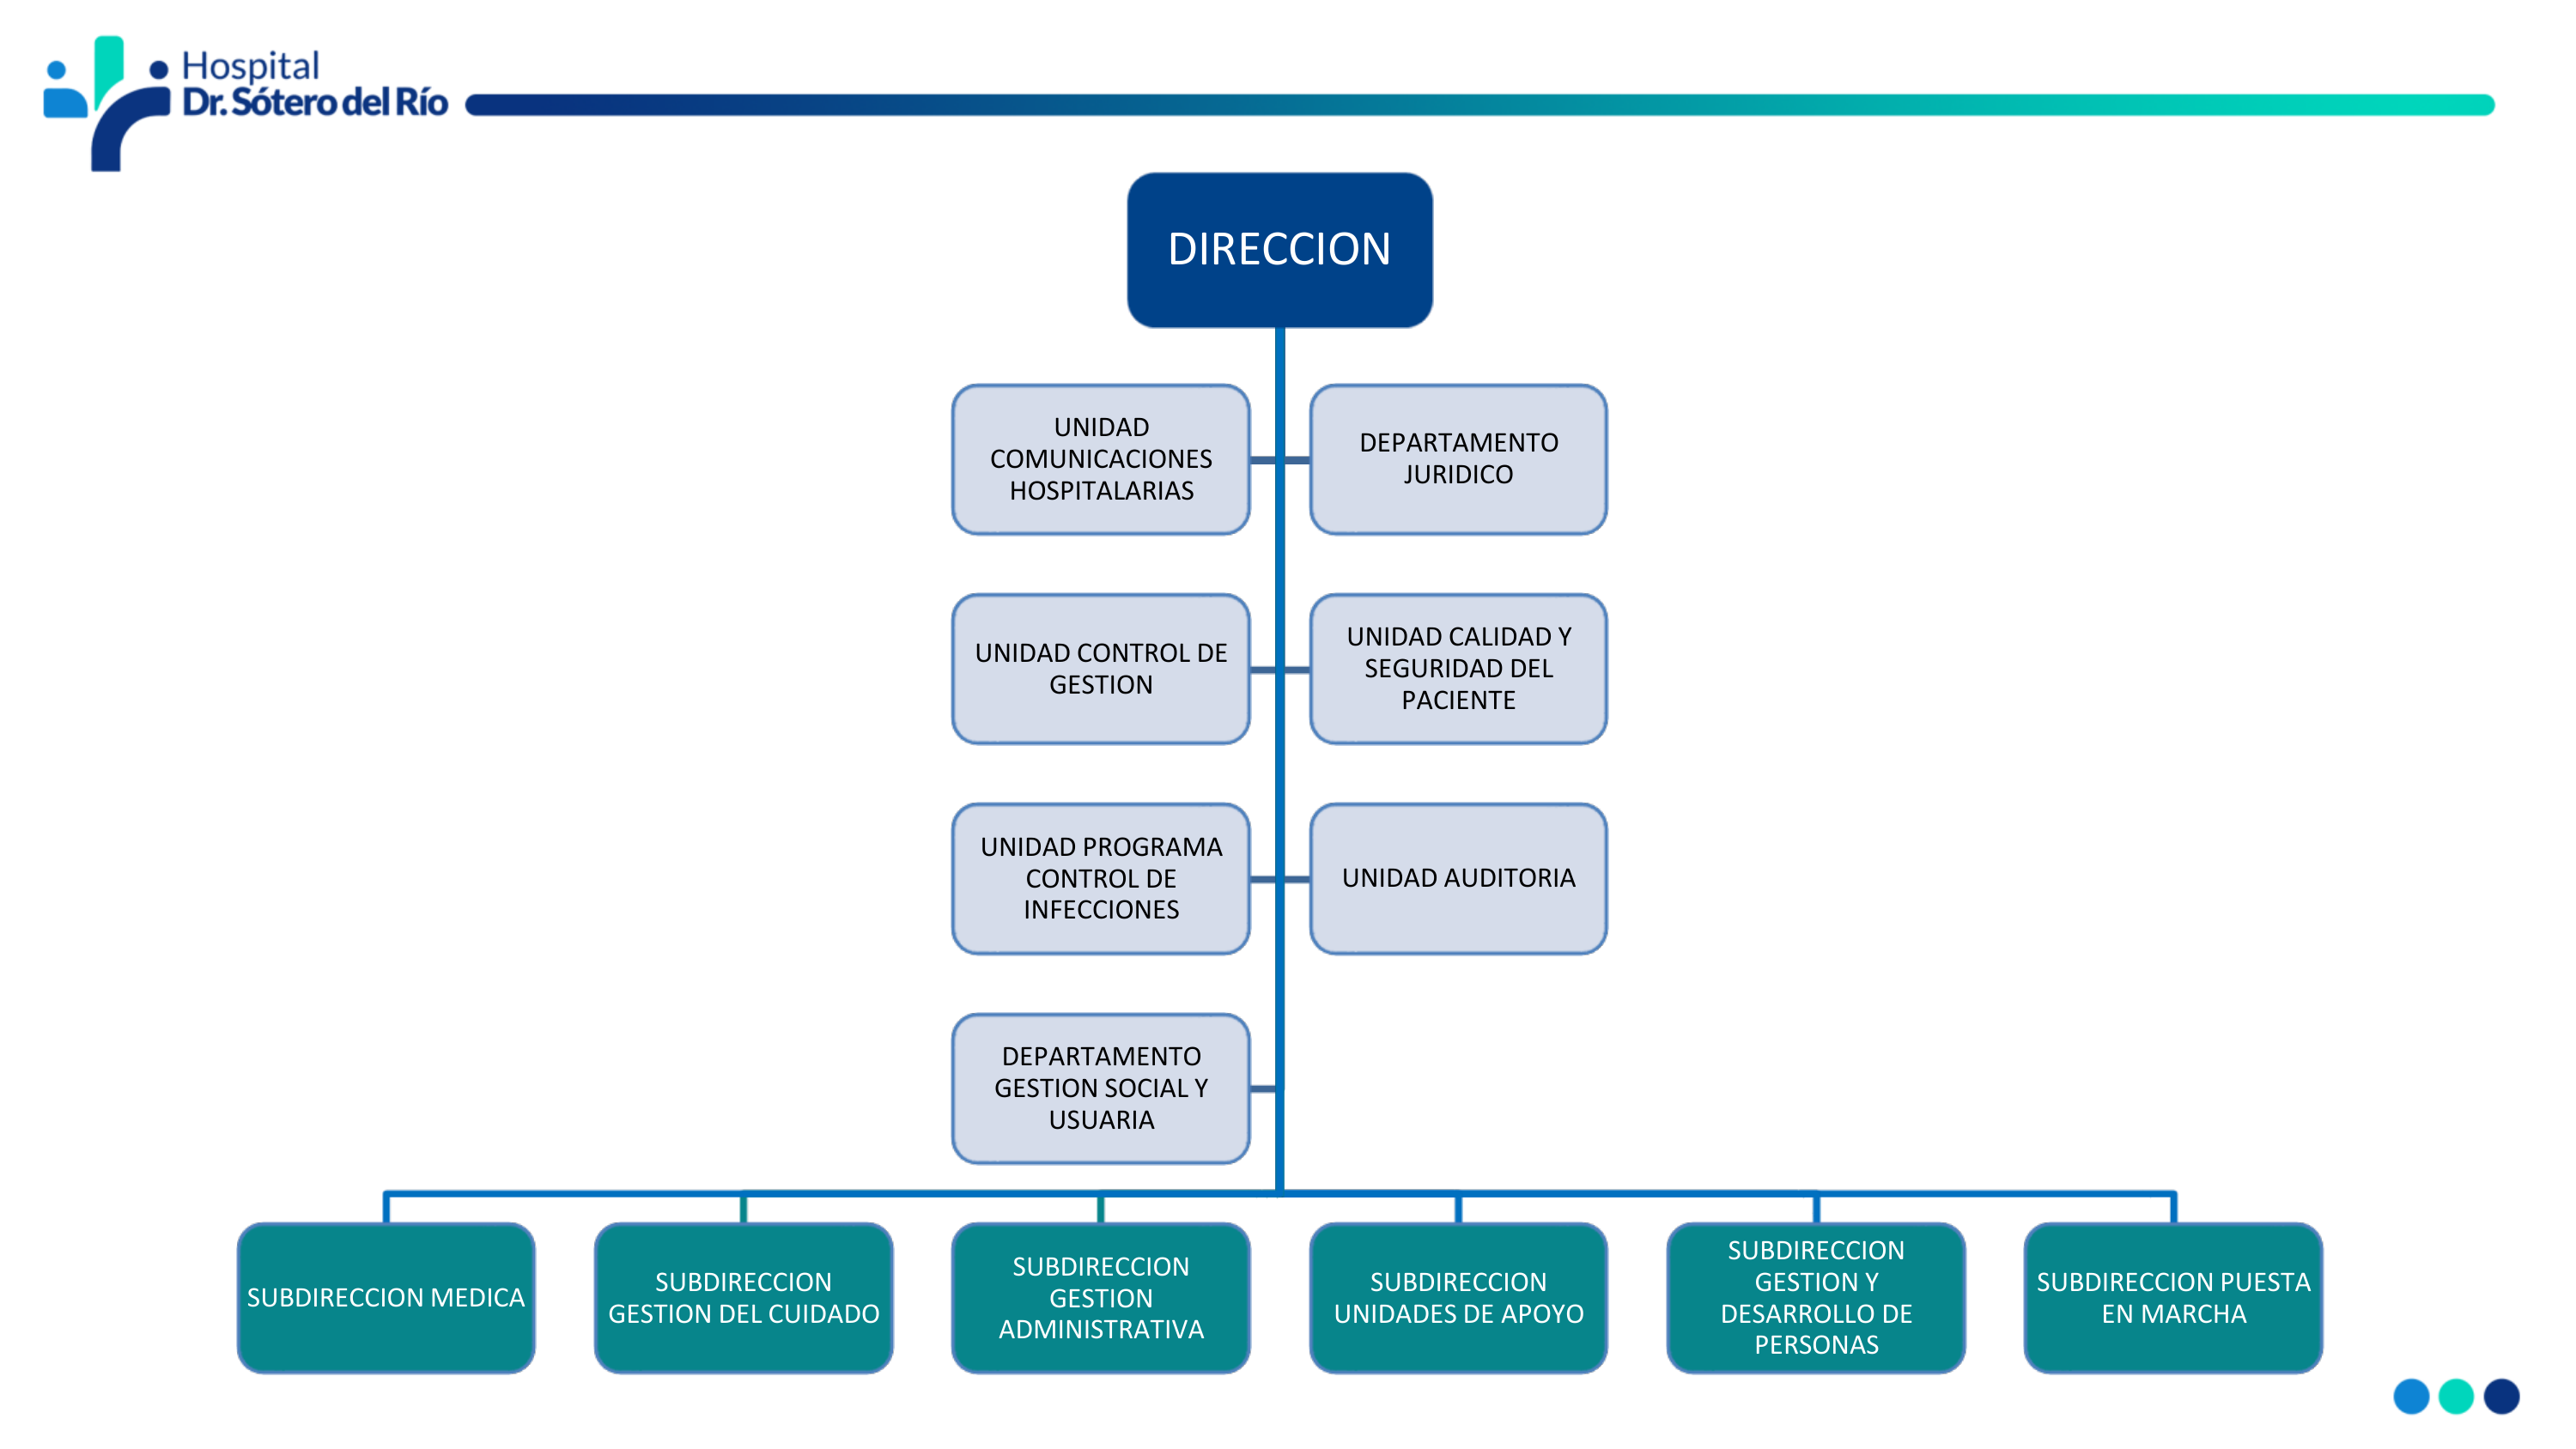
\includegraphics[width=\textwidth]{figures/organigrama_hsr-01.png}
    \caption{Organigrama del Complejo Asistencial Dr.~Sótero del Río.}
    \label{fig:organigrama}
\end{figure}

Para el proyecto resultan relevantes las funciones del equipo clínico de
oncología pediátrica. Este equipo entrega al cuidador las indicaciones de alta,
lo educa sobre signos de alerta y síntomas frecuentes y revisa la evolución del
paciente en cada control.

\section[Descripción del Área de Estudio]{Descripción del área de estudio}

\subsection*{Funciones y cargos relacionados con el proyecto}

El área de estudio es el cuidado domiciliario del paciente oncológico pediátrico
en la etapa posterior al alta. En ella participan cuatro actores. El equipo
clínico del hospital define los criterios médicos y las indicaciones de cuidado.
Los académicos de Enfermería de la Universidad del Bío-Bío, contraparte clínica
del proyecto, levantan la problemática, entregan los contenidos educativos y
definen los criterios de alerta. Las tesistas de Enfermería adaptan ese material
a un lenguaje comprensible para las familias. El cuidador principal, por último,
es quien observa al paciente, registra su evolución y aplica las indicaciones en
el hogar.

\subsection*{Objetivo del área}

El área busca dar continuidad al cuidado fuera del hospital. Su foco está en el
periodo entre controles, cuando el cuidador debe registrar antecedentes, resolver
dudas con información confiable y reconocer los signos que obligan a contactar
al equipo de salud o a acudir a urgencia.

\subsection*{Estructura organizativa del área y descripción de funciones}

Las funciones del área se reparten en tres niveles. El equipo clínico educa al
cuidador en el alta y en los controles, y revisa la evolución del paciente. La
contraparte de Enfermería traduce los criterios clínicos en contenidos educativos
y reglas de alerta. El cuidador ejecuta el seguimiento diario y lleva los
antecedentes a cada control.

\section[Descripción de la Problemática]{Descripción de la problemática}

\subsection{Situación actual del proceso de negocio}

Hoy la educación del cuidador se basa en indicaciones verbales, manuales
impresos, charlas y material que se entrega en el alta o en los controles. Una
vez en casa, el cuidador observa el estado general del paciente, anota sus
síntomas y aplica las indicaciones recibidas.

Cuando aparece una duda, como fiebre, dolor, vómitos o decaimiento, el cuidador
debe interpretar por sí mismo la información disponible y decidir si basta con
observar, si corresponde llamar al equipo clínico o si debe acudir a urgencia.
Esa decisión se toma bajo presión emocional y sin una fuente única de información
validada.

El registro de antecedentes tampoco sigue un formato. Los síntomas quedan en
cuadernos, mensajes, fotografías o en la memoria del cuidador, de modo que en el
control siguiente el equipo de salud debe reconstruir la evolución a partir de un
relato incompleto. La Figura~\ref{fig:proceso-negocio-actual} modela este
proceso en notación BPMN.

\begin{figure}[H]
    \centering
    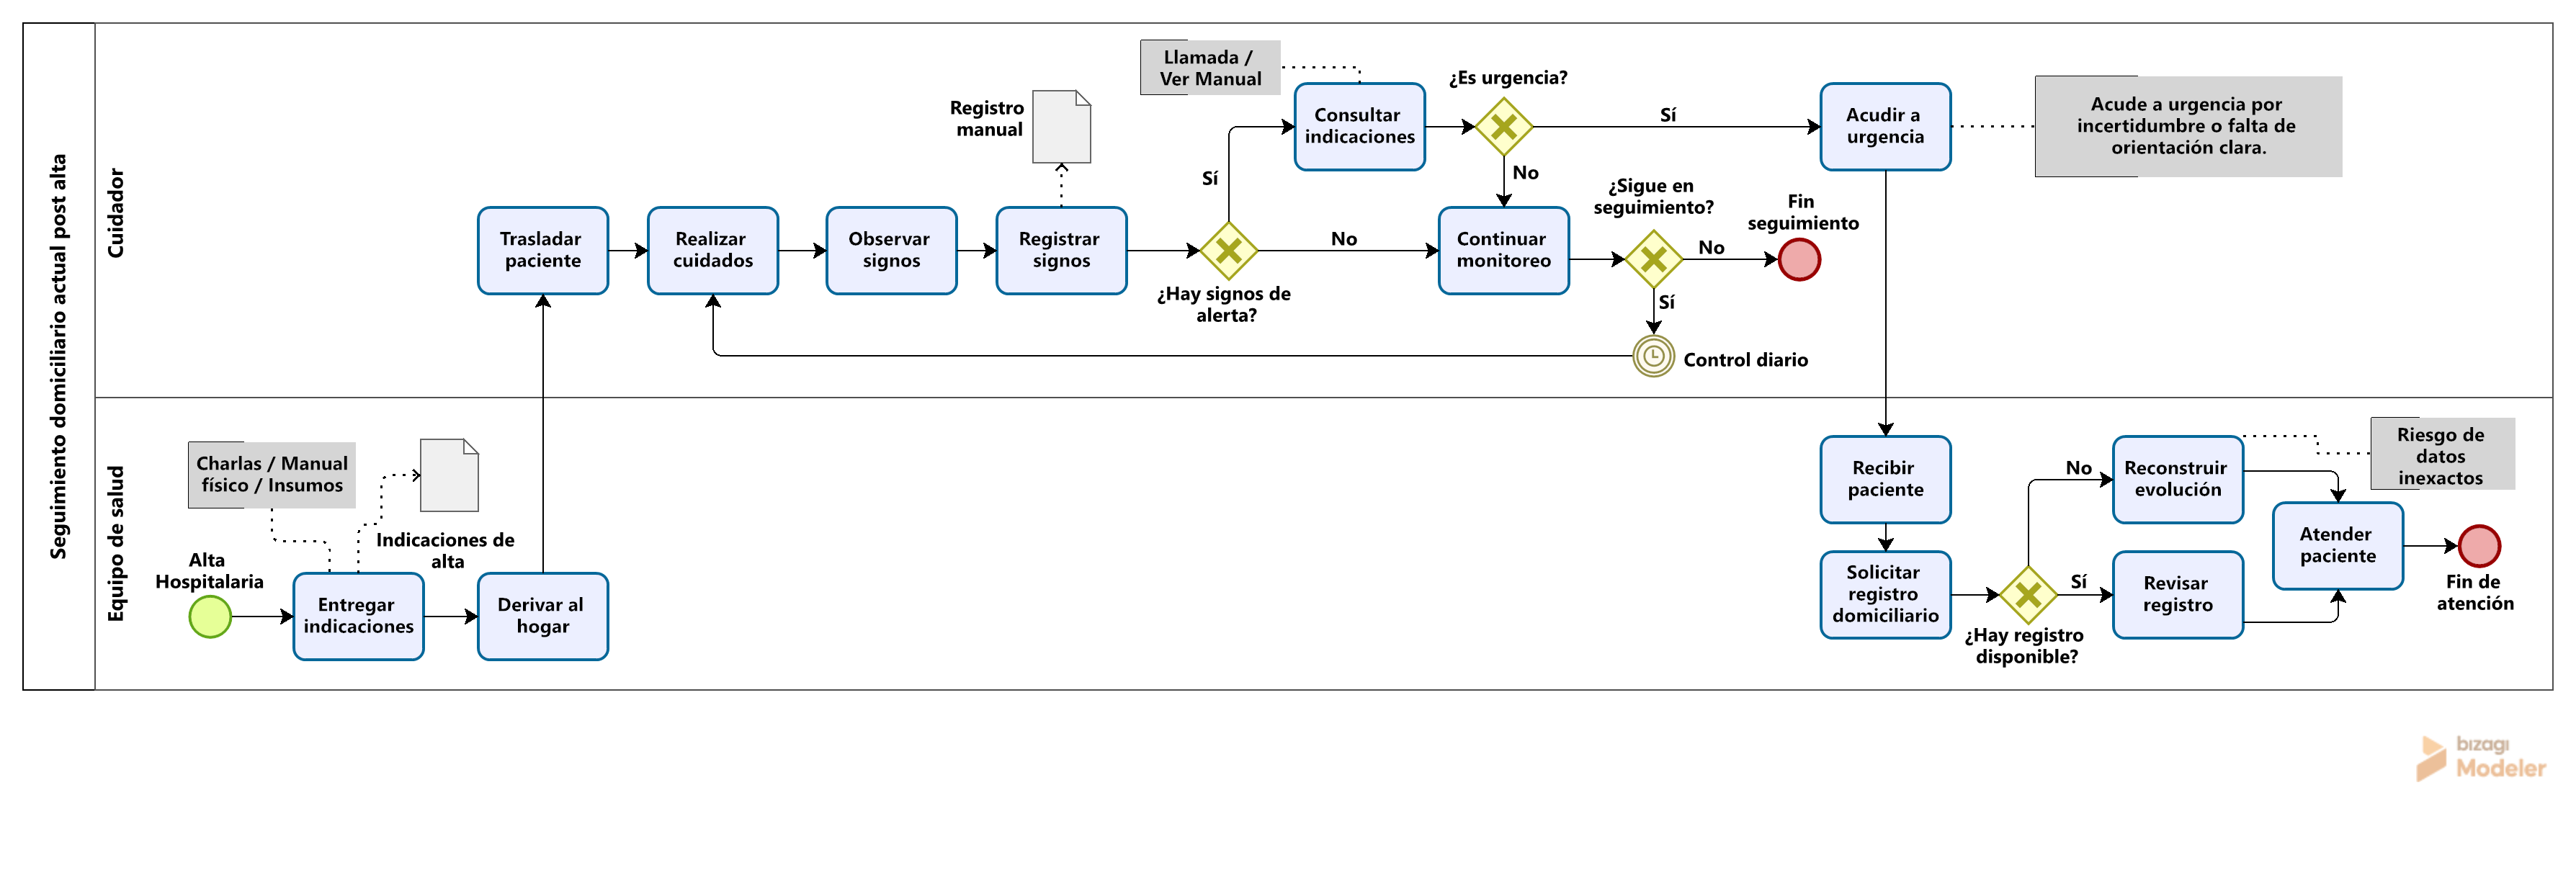
\includegraphics[width=\textwidth]{figures/proceso_negocio_actual.png}
    \caption{Proceso de negocio actual del seguimiento domiciliario.}
    \label{fig:proceso-negocio-actual}
\end{figure}

La literatura respalda la relevancia de este escenario. Los cuidadores de
pacientes oncológicos pediátricos presentan altos niveles de fatiga y sobrecarga
\citep{lewandowska_2022}, y las plataformas digitales de educación en cáncer
mejoran el conocimiento y la adherencia cuando la información está disponible en
el momento en que surge la duda \citep{nair_2017}. A su vez, el registro
estructurado de síntomas con escalas validadas como ESAS entrega al equipo
clínico antecedentes más confiables que el relato del cuidador
\citep{arnis_2024}, y los sistemas de apoyo a la decisión en el cuidado
domiciliario pediátrico favorecen la detección temprana de situaciones de riesgo
\citep{lau_2025}.

\subsection{Problemas detectados}

El problema central es la ausencia de una herramienta que apoye al cuidador en
tres tareas: registrar de forma ordenada la evolución del paciente, consultar
información educativa validada y reconocer a tiempo los signos de alerta. De él se
desprenden los siguientes problemas específicos.

\begin{enumerate}
    \item La información educativa está dispersa entre indicaciones verbales,
    manuales impresos y lo que el cuidador recuerda.
    \item Los síntomas registrados en el hogar no quedan ordenados ni disponibles
    para los controles.
    \item El cuidador no siempre distingue cuándo un síntoma requiere solo
    observación, una consulta o atención urgente.
    \item No existe un canal que resuelva dudas frecuentes con respuestas breves y
    validadas.
    \item El equipo clínico conoce la evolución entre controles solo a través de
    un relato no estandarizado.
\end{enumerate}

Estos problemas afectan a tres grupos. El cuidador vive el seguimiento con
incertidumbre y sobrecarga. El paciente queda expuesto a que un signo de alerta
se detecte tarde. El equipo clínico, por su parte, trabaja con información
domiciliaria incompleta.

De este diagnóstico nace el objetivo del sistema, que es entregar al cuidador
principal una aplicación móvil que centralice la información educativa validada,
registre de forma estructurada los signos y síntomas del paciente y lo oriente
ante signos de alerta, para dar continuidad a la atención entre el hospital y el
hogar.

\addtocontents{toc}{\protect\setcounter{tocdepth}{2}}


\addtocontents{toc}{\protect\setcounter{tocdepth}{1}}
\chapter[Definición del Proyecto]{Definición Proyecto}

\section[Objetivos del Proyecto]{Objetivos del proyecto}

\subsection{Objetivo general}

Desarrollar una solución móvil de apoyo integral a cuidadores de pacientes
oncológicos pediátricos para un centro hospitalario de alta complejidad, que
centralice herramientas de registro, seguimiento, consulta y orientación para
facilitar la continuidad del cuidado en el hogar.

\subsection{Objetivos específicos}

\begin{enumerate}
    \item Analizar las necesidades de información del cuidador principal y los
    flujos del cuidado domiciliario, a partir de los contenidos y criterios
    clínicos entregados por el equipo de Enfermería, para fundamentar la
    especificación funcional y no funcional del software.
    \item Diseñar la arquitectura de la solución móvil centrada en el cuidador,
    con su modelo de datos, servicios lógicos e interfaz de usuario, de modo que
    permita gestionar perfiles, registrar el seguimiento domiciliario y consultar
    el historial, priorizando la facilidad de uso y la seguridad de la
    información.
    \item Implementar los módulos que permiten al cuidador acceder a contenidos
    educativos validados, registrar los signos y síntomas del paciente, recibir
    orientación mediante alertas de semaforización clínica y gestionar
    recordatorios, con sincronización y respaldo en el servidor disponibles incluso
    sin conexión.
    \item Validar técnicamente el prototipo mediante pruebas automatizadas,
    verificando su conformidad con la especificación de requerimientos.
\end{enumerate}

\section[Ambiente de Ingeniería de Software]{Ambiente de Ingeniería de Software}

\subsection{Metodología de desarrollo}

El proyecto adopta Scrum de forma adaptada a un equipo de dos desarrolladoras y
a un plazo académico. Los requerimientos se expresan como historias de usuario
con criterios de aceptación, se estiman en puntos y se ordenan en un
\emph{product backlog} según su prioridad clínica y sus dependencias técnicas.
Scrum se elige porque permite entregar una versión funcional al cierre de cada
sprint, mostrarla a la contraparte y ajustar el alcance con lo aprendido.

El desarrollo se organiza en tres sprints. La Tabla~\ref{tab:sprints} resume su
foco y su calendario.

\begin{table}[H]
\centering
\small
\tablazebra
\caption{Organización del desarrollo en sprints.}
\label{tab:sprints}
\begin{tabularx}{\textwidth}{P{0.55}P{0.85}P{1.60}}
\toprule
\filaencabezado \encab{Sprint} & \encab{Periodo} & \encab{Foco} \\
\midrule
Sprint 1 & 26 ago -- 15 sep 2026 &
Flujo principal: acceso, cifrado de datos, gestión de pacientes, registro
clínico con clasificación de alertas e historial. \\
Sprint 2 & 16 sep -- 20 oct 2026 &
Rutina del cuidador: panel principal, exportación, biblioteca educativa,
asistente de orientación, preguntas frecuentes, recordatorios y listas de
verificación. \\
Sprint 3 & 21 oct -- 13 nov 2026 &
Integración: datos por paciente, aislamiento de la información, navegación
definitiva y funcionamiento sin conexión. \\
\bottomrule
\end{tabularx}
\end{table}

Cada sprint comienza con la selección de historias del backlog y termina con una
versión instalable (APK) que se revisa con la contraparte de Enfermería. La
contraparte valida la pertinencia de los contenidos, los textos y los criterios
de alerta, mientras que el docente guía supervisa el avance del proyecto.

\subsection{Técnicas y notaciones}

\begin{itemize}
    \item \emph{Historias de usuario} con criterios de aceptación, para expresar
    los requerimientos desde la perspectiva del cuidador.
    \item \emph{BPMN 2.0}, para modelar el proceso de seguimiento actual y el
    proceso futuro con la aplicación.
    \item \emph{UML 2.0}, en particular diagramas de casos de uso, para
    representar la interacción entre los actores y el sistema.
    \item \emph{Modelo entidad-relación}, para el modelo conceptual de datos, y
    esquema relacional de PostgreSQL para el diseño físico.
    \item \emph{Prototipos de alta fidelidad} en Figma, para validar la interfaz
    con la contraparte antes de construirla.
\end{itemize}

\subsection{Estándares de documentación}

La especificación de requerimientos se basa en IEEE~Std~830-1998
\citep{ieee_830_1998} y la documentación de pruebas en IEEE~Std~829-1998
\citep{ieee_829_1998}. Los atributos de calidad del producto toman como
referencia el modelo ISO/IEC~9126. En el código se sigue la guía de estilo de
Dart, verificada con flutter analyze, y los mensajes de
\emph{commit} siguen la convención \emph{Conventional Commits} en español.

\subsection{Tecnologías y herramientas de apoyo}

La aplicación se construye con Flutter \citep{flutter_2026}, que permite
compilar para Android e iOS desde una sola base de código en Dart y ofrece
componentes Material~3 listos para interfaces accesibles. Frente a Kotlin
nativo, evita duplicar el desarrollo para cada plataforma, y frente a React
Native, entrega un rendimiento más estable al no depender de puentes nativos.
Como backend se desarrolla una API REST propia con Node.js
\citep{nodejs_2026} y Express \citep{express_2026}, que persiste los datos en
una base relacional PostgreSQL \citep{postgresql_2026}. Ambos servicios se
empaquetan con Docker Compose \citep{docker_2026} y se destinan a ejecutarse como
contenedores Podman \citep{podman_2026} en el servidor que la Universidad del
Bío-Bío dispone para proyectos de título. Esta arquitectura responde al
requerimiento del profesor guía de contar con un backend y una base de datos
propios, y entrega control total sobre los datos y su cifrado a cambio de
asumir la operación del servidor. La Tabla~\ref{tab:herramientas} detalla el
propósito de cada herramienta.

\begin{table}[H]
\centering
\small
\tablazebra
\caption{Tecnologías y herramientas utilizadas en el desarrollo.}
\label{tab:herramientas}
\begin{tabularx}{\textwidth}{P{0.75}P{1.25}}
\toprule
\filaencabezado \encab{Tecnología o herramienta} & \encab{Propósito en el proyecto} \\
\midrule
Flutter y Dart & Construcción de la aplicación móvil para Android e iOS. \\
Riverpod & Gestión del estado y separación entre la lógica de datos y la
presentación \citep{riverpod_2026}. \\
go\_router & Navegación entre pantallas y redirección según el estado de la
sesión \citep{go_router_2026}. \\
Node.js 22 y Express 5 & API REST que atiende a la aplicación, valida las
solicitudes y custodia la clave de cifrado de cada usuario. \\
PostgreSQL 15 & Base de datos relacional que almacena los datos del cuidador, los
pacientes y sus registros como texto cifrado. \\
jsonwebtoken y bcryptjs & Sesión con tokens JWT y almacenamiento de las
contraseñas como \emph{hash} bcrypt. \\
nodemailer y SMTP & Envío de los correos de verificación y de recuperación de
acceso. \\
ffmpeg & Generación de las miniaturas de los videos de la biblioteca. \\
Docker y Docker Compose & Empaquetado y ejecución local de la API y la base de
datos. \\
Podman & Ejecución de los contenedores en el servidor de la universidad (destino
del despliegue). \\
DBeaver & Inspección de la base de datos durante el desarrollo. \\
cryptography y flutter\_secure\_storage & Cifrado AES-256-GCM de los datos
sensibles y resguardo de la clave en el dispositivo \citep{cryptography_dart_2026}. \\
flutter\_local\_notifications & Programación de los recordatorios como
notificaciones locales. \\
pdf y excel & Generación de los informes exportables del historial. \\
Git y GitHub & Control de versiones y respaldo del código, con una rama por
semana de trabajo. \\
Figma & Diseño de los prototipos de interfaz. \\
flutter\_test & Ejecución de la suite de pruebas automatizadas de la aplicación. \\
Jest y supertest & Pruebas de la API contra una base PostgreSQL real. \\
\bottomrule
\end{tabularx}
\end{table}

\section[Definiciones, Siglas y Abreviaciones]{Definiciones, siglas y abreviaciones}

\begingroup
\small
\tablazebra
\begin{xltabular}{\textwidth}{P{0.50}P{1.50}}
    \caption{Definiciones, siglas y abreviaciones.}
    \label{tab:siglas}\\
    \toprule
    \filaencabezado \encab{Término} & \encab{Definición} \\
    \midrule
    \endfirsthead
    \rowcolor{white}\multicolumn{2}{@{}l}{\footnotesize\itshape Tabla \thetable{} (continuación)} \\
    \toprule
    \filaencabezado \encab{Término} & \encab{Definición} \\
    \midrule
    \endhead
    \midrule
    \rowcolor{white}\multicolumn{2}{r@{}}{\footnotesize\itshape Continúa en la página siguiente} \\
    \endfoot
    \bottomrule
    \endlastfoot
    AES-256-GCM & Algoritmo de cifrado simétrico con clave de 256 bits en modo
    Galois/Counter, que además de cifrar verifica la integridad del dato. \\
    APK & Archivo de instalación de aplicaciones para Android. \\
    Backlog & Lista priorizada de historias de usuario pendientes de desarrollo. \\
    BPMN & Business Process Model and Notation, notación para modelar procesos
    de negocio. \\
    Cuidador principal & Persona que asume el cuidado diario del paciente en el
    hogar y usuario de la aplicación. \\
    CU & Caso de uso. \\
    ESAS & Edmonton Symptom Assessment System, escala que valora la intensidad de
    los síntomas de 0 a 10. \\
    HMAC & Hash-based Message Authentication Code, código de autenticación de
    mensajes basado en una función \emph{hash}; el servidor lo usa para guardar
    el correo de respaldo sin almacenarlo en claro. \\
    HTTP / HTTPS & Protocolo de transferencia de hipertexto, sin cifrar o con
    cifrado de transporte, que usa la aplicación para comunicarse con la API. \\
    HU & Historia de usuario. \\
    JSON & JavaScript Object Notation, formato de texto para intercambiar datos
    entre la aplicación y la API. \\
    JWT & JSON Web Token, token firmado que identifica la sesión del usuario en
    cada solicitud a la API. \\
    Motor de reglas & Componente que aplica condiciones predefinidas para
    clasificar un registro o elegir una respuesta, sin inteligencia artificial
    generativa. \\
    Offline-first & Enfoque de diseño en que la aplicación funciona sin conexión
    y sincroniza sus datos cuando recupera la red. \\
    Podman & Motor de contenedores sin demonio, compatible con Docker, que se
    usa en el servidor de la universidad. \\
    PINDA & Programa Infantil Nacional de Drogas Antineoplásicas del Ministerio
    de Salud de Chile. \\
    REST / API & Estilo de interfaz de servicios web sobre HTTP / interfaz de
    programación de aplicaciones. \\
    RF / RNF & Requerimiento funcional / requerimiento no funcional. \\
    Semaforización & Clasificación del nivel de riesgo en tres colores: verde
    (normal), amarillo (alerta) y rojo (crítico). \\
    SMTP & Simple Mail Transfer Protocol, protocolo con que el servidor envía los
    correos de verificación y recuperación. \\
    Sprint & Periodo fijo de trabajo al final del cual se entrega una versión
    funcional del producto. \\
    TRL & Technology Readiness Level. El nivel~3 corresponde a una prueba de
    concepto validada en un entorno de desarrollo. \\
    UCP & Use Case Points, técnica de estimación de tamaño basada en casos de
    uso. \\
    VAN / TIR & Valor actual neto / tasa interna de retorno. \\
\end{xltabular}
\endgroup

\addtocontents{toc}{\protect\setcounter{tocdepth}{2}}

% Capítulos fuera del alcance según índice objetivo Word (archivos en disco):
\iffalse
\chapter{Estado del Arte}

La salud móvil (mHealth) ha emergido como una línea consolidada de intervención
en el cuidado oncológico, especialmente para la educación y el seguimiento de
pacientes fuera del entorno hospitalario. La evidencia indica que las
plataformas digitales pueden mejorar el conocimiento y la adherencia de los
cuidadores, facilitando el acceso a información estructurada en el momento en
que surge la duda \citep{nair_2017}. En el contexto pediátrico, el cuidador
principal asume un rol observador y registrador de la evolución del paciente,
por lo que disponer de herramientas que ordenen esa información reduce la carga
cognitiva y emocional del seguimiento domiciliario \citep{lewandowska_2022}.

En relación con el registro y seguimiento de síntomas, la literatura destaca la
utilidad de escalas validadas como el Edmonton Symptom Assessment System (ESAS)
y de aplicaciones que permiten el registro longitudinal de signos vitales y
síntomas en el hogar. Estos antecedentes estructurados se constituyen en
insumos valiosos para la consulta clínica, pues permiten al equipo de salud
revisar la evolución del paciente entre controles en lugar de depender
únicamente del relato del cuidador \citep{arnis_2024}. En el mismo sentido, el
uso de sistemas de apoyo a la decisión y triaje en aplicaciones de cuidado
domiciliario pediátrico ha mostrado resultados favorables en la detección
temprana de situaciones que requieren contacto con el equipo de salud
\citep{lau_2025}.

En oncología pediátrica, los programas nacionales y las sociedades científicas
coinciden en la importancia de la educación del cuidador y en la delimitación
estricta de los contenidos: la información entregada debe ser acotada, validada
y no debe sustituir la evaluación profesional \citep{minsal_sf,pohema_seop_sf}.
En Chile, el Programa PINDA y sus centros de referencia definen protocolos de
emergencia y criterios de derivación que constituyen la base clínica sobre la
que la aplicación construye sus reglas de semaforización
\citep{pinda_estadisticas_2026}.

Finalmente, la evidencia respalda que las intervenciones de salud móvil
dirigidas a cuidadores de pacientes pediátricos oncológicos son viables y bien
aceptadas cuando la interfaz es simple, el lenguaje es comprensible y la
información se encuentra disponible incluso sin conexión
\citep{paho_oms_sf,mskcc_sf,idsa_sf,aepap_sf}. Sobre esta base, el proyecto
OnCuidar adopta un enfoque de seguridad por diseño y funcionamiento offline
-first, alineado con las recomendaciones de organismos internacionales de salud
para el uso de tecnologías digitales en pediatría.
\chapter{Evaluación de Plataformas}

La elección del stack tecnológico se realizó comparando las alternativas
disponibles en tres dimensiones: framework de desarrollo móvil, backend como
servicio y estrategia de almacenamiento y notificaciones.

\section{Framework de desarrollo móvil}

Se evaluaron Flutter, Kotlin nativo (Android) y React Native. Kotlin nativo
garantiza el máximo desempeño y acceso directo a las APIs de Android, pero
restringe la solución a una única plataforma y aumenta el esfuerzo de desarrollo
para una segunda plataforma. React Native permite compartir código entre
plataformas, pero introduce dependencias de puentes nativos y mayor variabilidad
en el desempeño. Flutter se selecciona porque permite construir interfaces
consistentes en Android e iOS desde una única base de código en Dart, ofrece un
sistema de widgets con Material 3 que acelera el desarrollo de interfaces
accesibles y cuenta con un ecosistema maduro de paquetes (Riverpod, go\_router,
cryptography). Para un proyecto académico que debe demostrar resultados en
plazos acotados, Flutter presenta el mejor equilibrio entre velocidad de
desarrollo, calidad visual y soporte.

\begin{table}[H]
\centering
\small
\tablazebra
\caption{Comparación de frameworks de desarrollo móvil.}
\label{tab:comparacion-frameworks}
\begin{tabularx}{\textwidth}{P{0.78}P{1.07}P{1.07}P{1.08}}
\toprule
\filaencabezado \encab{Criterio} & \encab{Flutter} & \encab{Kotlin nativo} & \encab{React Native} \\
\midrule
Plataformas &
Android e iOS con una base de código &
Solo Android &
Android e iOS con puentes nativos \\
Desempeño &
Alto (compila a nativo) &
Máximo &
Variable (depende del puente) \\
Ecosistema de paquetes &
Maduro (Riverpod, go\_router, cryptography) &
Maduro para Android &
Amplio, con mayor variabilidad \\
Velocidad de desarrollo &
Alta (Material 3, widgets) &
Media &
Media \\
\bottomrule
\end{tabularx}
\end{table}

\section{Backend como servicio}

Se compararon Firebase, Supabase y un backend propio. Un backend propio ofrece
control total, pero exige mantener servidores, autenticación, seguridad y
despliegue, lo que excede el alcance y las horas disponibles. Supabase, basado
en PostgreSQL, es una alternativa válida de open source, pero requiere
configuración adicional de políticas de seguridad y su ecosistema de integración
móvil es menor. Firebase se selecciona por su integración nativa con Flutter, la
sincronización en tiempo real de Cloud Firestore, la persistencia local
integrada que habilita el modo offline-first y la disponibilidad del plan
gratuito (Spark) suficiente para un piloto académico.

\section{Almacenamiento local}

Se evaluó el uso exclusivo de Room sobre SQLite (opción considerada en el
anteproyecto) frente a Firestore. Room ofrece almacenamiento 100~\% local y
máximo control, pero dificulta la sincronización y la persistencia en múltiples
dispositivos. Firestore, si bien es un servicio en la nube, compensa la
dependencia de red con tres mecanismos: persistencia local habilitada, caché de
metadatos en SharedPreferences y caché de archivos con auto-descarga. Esta
combinación entrega un comportamiento equivalente al offline esperado por el
anteproyecto, sumando el beneficio de la sincronización entre el dispositivo del
cuidador y los servicios de respaldo.

\section{Notificaciones}

Se evaluaron notificaciones push con FCM frente a notificaciones locales. FCM
permite alertar al usuario incluso con la aplicación cerrada y desde el
servidor, pero exige infraestructura adicional, manejo de permisos de plataforma
y puede fallar sin conexión. Para los recordatorios de valoración diaria del
paciente se opta por notificaciones locales (flutter\_local\_notifications),
re-planificadas al iniciar sesión: no dependen de red, respetan horas exactas
mediante SCHEDULE\_EXACT\_ALARM y cubren completamente el requerimiento
de recordar al cuidador la valoración diaria.

\section{Conclusión de la evaluación}

Como conclusión, el stack elegido —Flutter/Dart con Riverpod y go\_router,
Firebase (Auth, Firestore, Functions, Storage) y notificaciones locales—
satisface los requerimientos funcionales y no funcionales del proyecto, es de
costo cero, está ampliamente documentado y permite un funcionamiento offline
-first con seguridad por diseño.
\fi

\chapter[Especificación de Requerimientos de Software]{Especificación de Requerimientos de Software}

\emph{Adaptación basada en IEEE Std 830-1998, Software Requirements
Specifications \citep{ieee_830_1998}.}

\section[Alcances]{Alcances}

OnCuidar es una aplicación móvil para el cuidador principal de un paciente
oncológico pediátrico. Se diferencia de las aplicaciones genéricas de salud en
que su contenido educativo y sus criterios de alerta provienen del equipo de
Enfermería que acompaña el proyecto, en que funciona sin conexión y en que cifra
los datos sensibles en el propio dispositivo.

\subsection*{Funcionalidades dentro del alcance}

\begin{itemize}
    \item Crear una cuenta con los datos del cuidador, del paciente, del centro
    de salud y del contacto de emergencia, e iniciar sesión de forma segura.
    \item Gestionar uno o más pacientes y elegir cuál es el paciente activo.
    \item Registrar signos vitales, síntomas de la escala ESAS y observaciones,
    y clasificar cada registro en los niveles normal, alerta o crítico.
    \item Consultar el historial de registros y exportarlo a PDF y Excel.
    \item Consultar una biblioteca de videos, guías, infografías y documentos,
    disponible sin conexión.
    \item Resolver dudas frecuentes mediante un asistente de orientación y una
    sección de preguntas frecuentes.
    \item Programar recordatorios con notificaciones locales.
\end{itemize}

\subsection*{Funcionalidades fuera del alcance}

\begin{itemize}
    \item Diagnosticar, indicar tratamientos o calcular dosis de medicamentos.
    \item Reemplazar la evaluación del equipo de salud o la atención presencial.
    \item Enviar los registros directamente al hospital o integrarse con su ficha
    clínica electrónica.
    \item Generar respuestas con inteligencia artificial generativa.
    \item Ofrecer una aplicación web o un panel de administración para el equipo
    clínico.
\end{itemize}

\section[Objetivo del Software]{Objetivo del software}

\addtocontents{toc}{\protect\setcounter{tocdepth}{1}}
\subsection{Objetivo general}
\addtocontents{toc}{\protect\setcounter{tocdepth}{2}}

El software gestiona la información del seguimiento domiciliario del paciente
oncológico pediátrico, compuesta por sus signos vitales, síntomas, historial,
recordatorios y contenidos educativos, para apoyar al cuidador en el proceso de
cuidado en el hogar. Con ello logra un registro ordenado y trazable de la
evolución del paciente y una orientación oportuna ante signos de alerta.

\addtocontents{toc}{\protect\setcounter{tocdepth}{1}}
\subsection{Objetivos específicos}
\addtocontents{toc}{\protect\setcounter{tocdepth}{2}}

\begin{enumerate}
    \item Almacenar los antecedentes del cuidador y de sus pacientes, cifrando
    los datos sensibles antes de que salgan del dispositivo.
    \item Registrar la valoración clínica diaria del paciente y clasificar su
    nivel de alerta mediante un motor de reglas clínicas.
    \item Entregar contenido educativo validado y respuestas a dudas frecuentes,
    disponibles incluso sin conexión.
    \item Generar informes del historial en PDF y Excel para presentarlos en los
    controles clínicos.
    \item Recordar al cuidador las tareas de cuidado mediante notificaciones
    locales.
\end{enumerate}

\section[Descripción Global del Producto]{Descripción global del producto}

\subsection[Interfaz de Usuario]{Interfaz de usuario}

La interfaz está pensada para personas sin formación técnica ni clínica que
pueden usarla en momentos de estrés. Por eso emplea textos breves, botones
amplios y un lenguaje cotidiano. Sigue las pautas de Material~3 con una paleta
cálida basada en el dorado del lazo del cáncer infantil y la tipografía Nunito.

Todas las pantallas comparten una cabecera con degradado dorado y una barra de
navegación inferior con cinco accesos: Inicio, Chat, Registro, Aprende y
Perfil. El nivel de alerta se comunica siempre con el mismo código de colores,
verde para normal, amarillo para alerta y rojo para crítico, acompañado de un
ícono y un texto para no depender solo del color.

\subsection[Interfaz de Hardware]{Interfaz de hardware}

La aplicación se ejecuta en teléfonos Android e iOS compatibles con Flutter y no
requiere sensores ni periféricos especiales. Utiliza el almacenamiento interno
para la persistencia local de datos, la caché del contenido educativo y los
archivos exportados. Solicita permisos de notificaciones, de alarmas exactas y
de ejecución al reiniciar el dispositivo, para que los recordatorios se
disparen a la hora programada.

\subsection[Interfaz de Software]{Interfaz software}

La Tabla~\ref{tab:interfaz-software} detalla los productos de software con los
que se relaciona el sistema.

\begingroup
\small
\tablazebra
\begin{xltabular}{\textwidth}{P{1.25}P{0.85}P{0.80}P{1.10}}
    \caption{Productos de software con los que se relaciona el sistema.}
    \label{tab:interfaz-software}\\
    \toprule
    \filaencabezado \encab{Nombre} & \encab{Abreviación} & \encab{Versión} & \encab{Fuente} \\
    \midrule
    \endfirsthead
    \rowcolor{white}\multicolumn{4}{@{}l}{\footnotesize\itshape Tabla \thetable{} (continuación)} \\
    \toprule
    \filaencabezado \encab{Nombre} & \encab{Abreviación} & \encab{Versión} & \encab{Fuente} \\
    \midrule
    \endhead
    \midrule
    \rowcolor{white}\multicolumn{4}{r@{}}{\footnotesize\itshape Continúa en la página siguiente} \\
    \endfoot
    \bottomrule
    \endlastfoot
    Flutter SDK (Dart) & Flutter & Dart 3.12 & flutter.dev \\
    http & --- & 1.6.0 & pub.dev \\
    flutter\_riverpod & Riverpod & 3.4.2 & pub.dev \\
    go\_router & --- & 17.5.0 & pub.dev \\
    cryptography & --- & 2.9.0 & pub.dev \\
    flutter\_secure\_storage & --- & 9.2.4 & pub.dev \\
    flutter\_local\_notifications & --- & 22.3.1 & pub.dev \\
    flutter\_cache\_manager & --- & 3.4.4 & pub.dev \\
    connectivity\_plus & --- & 7.3.1 & pub.dev \\
    pdf & --- & 3.12.0 & pub.dev \\
    excel & --- & 4.0.6 & pub.dev \\
    video\_player & --- & 2.14.0 & pub.dev \\
    url\_launcher & --- & 6.3.2 & pub.dev \\
    share\_plus & --- & 12.0.2 & pub.dev \\
    Node.js & Node & 22 & nodejs.org \\
    Express & --- & 5.3.0 & npmjs.com \\
    PostgreSQL & Postgres & 15 & postgresql.org \\
    pg (cliente de PostgreSQL) & --- & 8.23.1 & npmjs.com \\
    bcryptjs & --- & 2.4.3 & npmjs.com \\
    jsonwebtoken & --- & 9.0.3 & npmjs.com \\
    nodemailer & --- & 6.10.1 & npmjs.com \\
    helmet & --- & 8.3.0 & npmjs.com \\
    cors & --- & 2.8.6 & npmjs.com \\
    Jest & --- & 29.7.0 & npmjs.com \\
    supertest & --- & 7.3.1 & npmjs.com \\
    Docker Compose y Podman & --- & --- & docker.com, podman.io \\ % REVISAR: versión instalada en el servidor
\end{xltabular}
\endgroup

\addtocontents{toc}{\protect\setcounter{tocdepth}{1}}
\subsection{Interfaces de comunicación}
\addtocontents{toc}{\protect\setcounter{tocdepth}{2}}

La aplicación se comunica con la API REST propia mediante HTTP, con mensajes en
formato JSON y autenticación por token JWT en cada solicitud. En el entorno del
servidor de la universidad se prevé servir la API sobre HTTPS. El contenido
educativo (videos, infografías y guías) lo sirve el mismo backend desde la ruta
/archivos y la aplicación lo descarga para su uso sin conexión. El
servidor envía los correos de verificación y recuperación mediante SMTP. La
aplicación abre llamadas telefónicas con el esquema tel: y direcciones
en Google Maps mediante enlaces web. No se definen protocolos propios.

\section[Requerimientos Específicos]{Requerimientos específicos}

\subsection[Requerimientos Funcionales del Sistema]{Requerimientos funcionales del sistema}

Los requerimientos funcionales se derivan de las historias de usuario del
backlog y se agrupan por módulo. La columna HU indica la historia de usuario que
da origen a cada requerimiento, lo que permite seguir su trazabilidad hasta las
pruebas.

\begingroup
\small
\tablazebra
\begin{xltabular}{\textwidth}{P{0.42}P{0.95}P{2.33}P{0.55}P{0.75}}
    \caption{Requerimientos funcionales del sistema.}
    \label{tab:requerimientos-funcionales}\\
    \toprule
    \filaencabezado \encab{ID} & \encab{Nombre} & \encab{Descripción} & \encab{HU} & \encab{Prioridad} \\
    \midrule
    \endfirsthead
    \rowcolor{white}\multicolumn{5}{@{}l}{\footnotesize\itshape Tabla \thetable{} (continuación)} \\
    \toprule
    \filaencabezado \encab{ID} & \encab{Nombre} & \encab{Descripción} & \encab{HU} & \encab{Prioridad} \\
    \midrule
    \endhead
    \midrule
    \rowcolor{white}\multicolumn{5}{r@{}}{\footnotesize\itshape Continúa en la página siguiente} \\
    \endfoot
    \bottomrule
    \endlastfoot
    \filagrupo{5}{Acceso y seguridad}
    RF-01 & Iniciar la aplicación &
    Mostrar una pantalla de carga y dirigir al panel principal si existe una
    sesión activa, o a la bienvenida si no la hay. & HU-01 & Crítica \\
    RF-02 & Crear cuenta &
    Registrar la cuenta con correo y contraseña junto con los datos del
    cuidador, del paciente, del centro de salud y del contacto de emergencia,
    validando los campos obligatorios y sus formatos. & HU-02 & Crítica \\
    RF-03 & Iniciar y cerrar sesión &
    Autenticar al cuidador, informar con claridad las credenciales inválidas,
    mantener la sesión abierta entre usos y cerrarla limpiando los datos
    locales. & HU-03 & Alta \\
    RF-04 & Recuperar acceso &
    Enviar al correo principal o al de respaldo un enlace de restablecimiento de
    contraseña de un solo uso, con una hora de vigencia. & HU-03 & Alta \\
    RF-05 & Cifrar datos sensibles &
    Cifrar en el dispositivo los datos personales y clínicos antes de enviarlos al
    servidor, obtener la clave de cada usuario desde el servidor que la custodia y
    bloquear el acceso a la clave al cerrar sesión. & HU-04 & Crítica \\
    RF-29 & Verificar correos por enlace &
    Enviar un enlace de verificación de un solo uso, con una hora de vigencia, al
    correo principal al registrarse o cambiarlo y al correo de respaldo; mostrar
    si el correo está verificado o pendiente, sin bloquear el uso de la
    aplicación, y permitir reenviar el enlace una vez por minuto como máximo. & HU-05 & Media \\
    \filagrupo{5}{Perfil y pacientes}
    RF-06 & Gestionar perfil del cuidador &
    Mostrar y editar los datos del cuidador, exigir la contraseña actual para
    cambiar un correo e indicar cuándo el nuevo correo está pendiente de
    verificación. & HU-05 & Alta \\
    RF-07 & Gestionar pacientes &
    Crear, editar, archivar y restaurar los pacientes del cuidador, con
    confirmación antes de archivar. & HU-06 & Crítica \\
    RF-08 & Seleccionar paciente activo &
    Elegir el paciente activo desde una lista, mostrar su nombre en el panel
    principal y conservar la selección al navegar o cerrar la aplicación. & HU-07 & Crítica \\
    RF-09 & Contactar al centro de salud &
    Iniciar una llamada al centro de salud del paciente y abrir su dirección en
    la aplicación de mapas. & HU-06 & Media \\
    RF-10 & Separar datos por paciente &
    Asociar registros y recordatorios al paciente activo
    y actualizar todas las vistas al cambiar de paciente. & HU-24 & Alta \\
    \filagrupo{5}{Registro clínico e historial}
    RF-11 & Registrar valoración clínica &
    Registrar hasta cuatro signos vitales opcionales (temperatura, frecuencia
    cardíaca, saturación de oxígeno y frecuencia respiratoria), la intensidad de
    los síntomas ESAS de 0 a 10 (sin síntoma, leve, moderado, severo e insoportable) y
    observaciones, rechazando valores fuera de
    rango físico. & HU-09 & Crítica \\
    RF-12 & Controlar tope diario &
    Distinguir registros programados y extra, y bloquear los programados cuando
    el paciente alcanza su tope diario, fijado en tres por defecto. & HU-09 & Crítica \\
    RF-13 & Clasificar nivel de alerta &
    Clasificar cada registro como normal, alerta o crítico según umbrales de
    signos vitales e intensidad de síntomas, y mostrar el motivo junto con la
    recomendación correspondiente. & HU-09 & Crítica \\
    RF-14 & Consultar historial &
    Listar en orden cronológico los registros del paciente activo, filtrarlos
    por fecha o nivel de alerta y mostrar el detalle de cada uno. & HU-10 & Alta \\
    RF-15 & Editar y eliminar registros &
    Modificar o eliminar los registros del día, con confirmación previa a la
    eliminación. & HU-11 & Media \\
    RF-16 & Exportar historial a PDF &
    Generar un informe PDF con los datos del paciente y sus registros en un rango
    de fechas, y permitir guardarlo o compartirlo. & HU-12 & Alta \\
    RF-17 & Exportar historial a Excel &
    Generar una planilla Excel con fecha, signos, síntomas, nivel y
    observaciones de cada registro en un rango de fechas, y permitir guardarla o
    compartirla. & HU-13 & Media \\
    RF-18 & Mostrar panel principal &
    Presentar el paciente activo, la fecha del último registro, un resumen de
    signos vitales, los registros del día, el nivel de alerta vigente y accesos
    directos a los módulos. & HU-08 & Alta \\
    \filagrupo{5}{Orientación}
    RF-19 & Consultar asistente &
    Responder por chat la consulta escrita del cuidador con la pregunta frecuente
    que mejor coincide por palabras clave, o con una respuesta de respaldo si no
    hay coincidencia. & HU-14 & Media \\
    RF-20 & Gestionar conversaciones &
    Guardar las conversaciones con un título automático, listarlas por última
    actividad y permitir continuarlas, renombrarlas y eliminarlas. & HU-15 & Baja \\
    RF-21 & Consultar preguntas frecuentes &
    Mostrar las preguntas frecuentes por categoría, con búsqueda por palabra
    clave que ignora tildes. & HU-16 & Baja \\
    \filagrupo{5}{Recordatorios}
    RF-22 & Gestionar recordatorios &
    Crear, editar, activar o desactivar y eliminar recordatorios de medicamento, medición,
    cita u otro tipo, únicos o recurrentes. & HU-17 & Alta \\
    RF-23 & Notificar recordatorios &
    Emitir una notificación local a la hora de cada recordatorio activo,
    cancelarlas al cerrar sesión y reprogramarlas al volver a iniciarla. & HU-18 & Media \\
    \filagrupo{5}{Educación}
    RF-24 & Consultar biblioteca &
    Mostrar el catálogo de videos, guías, infografías y documentos, con filtro
    por categoría, búsqueda por título, favoritos y estado de descarga. & HU-19 & Media \\
    RF-25 & Descargar contenido &
    Descargar el contenido educativo en segundo plano tras el primer ingreso,
    reintentar ante fallas de red y mostrar el progreso. & HU-20 & Alta \\
    RF-26 & Reproducir videos &
    Reproducir los videos educativos en horizontal y a pantalla inmersiva, con
    controles para reproducir, pausar, avanzar y retroceder 10 segundos, una barra
    de progreso y la reanudación desde donde quedó. & HU-21 & Media \\
    RF-27 & Ver guías e infografías &
    Mostrar las guías como recomendaciones en secciones con título y las
    infografías ampliadas sobre la pantalla, con zoom de hasta cinco veces. & HU-22 & Media \\
    \filagrupo{5}{Funcionamiento sin conexión}
    RF-28 & Operar sin conexión &
    Crear y consultar registros sin conexión, guardar las escrituras en una cola
    persistente que se reintenta al recuperar la red y avisar al cuidador cuando
    no hay conexión. & HU-27 & Alta \\
\end{xltabular}
\endgroup

\subsection[Interfaces Externas de Entrada]{Interfaces externas de entrada}

La Tabla~\ref{tab:entradas} agrupa los datos que ingresan al sistema.

\begingroup
\small
\tablazebra
\begin{xltabular}{\textwidth}{P{0.45}P{0.75}P{1.80}}
    \caption{Interfaces externas de entrada.}
    \label{tab:entradas}\\
    \toprule
    \filaencabezado \encab{Identificador} & \encab{Nombre del ítem} & \encab{Detalle de datos contenidos en el ítem} \\
    \midrule
    \endfirsthead
    \rowcolor{white}\multicolumn{3}{@{}l}{\footnotesize\itshape Tabla \thetable{} (continuación)} \\
    \toprule
    \filaencabezado \encab{Identificador} & \encab{Nombre del ítem} & \encab{Detalle de datos contenidos en el ítem} \\
    \midrule
    \endhead
    \midrule
    \rowcolor{white}\multicolumn{3}{r@{}}{\footnotesize\itshape Continúa en la página siguiente} \\
    \endfoot
    \bottomrule
    \endlastfoot
    DE\_01 & Datos de la cuenta & Correo electrónico, correo de respaldo,
    contraseña y confirmación de contraseña. \\
    DE\_02 & Datos del cuidador & Nombre completo, relación con el paciente,
    teléfono y dirección. \\
    DE\_03 & Datos del paciente & Nombre, RUT, edad, diagnóstico, fase de
    tratamiento y tope diario de registros. \\
    DE\_04 & Centro de salud y emergencia & Nombre, dirección y teléfono del
    centro de salud, nombre y teléfono del contacto de emergencia. \\
    DE\_05 & Credenciales de acceso & Correo electrónico y contraseña. \\
    DE\_06 & Valoración clínica & Tipo de registro, temperatura, frecuencia
    cardíaca, saturación de oxígeno, frecuencia respiratoria, síntomas con su
    intensidad y observaciones. \\
    DE\_07 & Consulta al asistente & Texto libre de la duda del cuidador. \\
    DE\_08 & Criterios de búsqueda & Palabras clave, categoría y rango de
    fechas. \\
    DE\_09 & Recordatorio & Título, descripción, tipo, fecha, hora, días de
    repetición y recurrencia. \\
\end{xltabular}
\endgroup

\subsection[Interfaces Externas de Salida]{Interfaces externas de salida}

La Tabla~\ref{tab:salidas} detalla las salidas del sistema y su medio.

\begingroup
\small
\tablazebra
\begin{xltabular}{\textwidth}{P{0.55}P{0.90}P{1.95}P{0.60}}
    \caption{Interfaces externas de salida.}
    \label{tab:salidas}\\
    \toprule
    \filaencabezado \encab{Identificador} & \encab{Nombre del ítem} & \encab{Detalle de datos contenidos en el ítem} & \encab{Medio} \\
    \midrule
    \endfirsthead
    \rowcolor{white}\multicolumn{4}{@{}l}{\footnotesize\itshape Tabla \thetable{} (continuación)} \\
    \toprule
    \filaencabezado \encab{Identificador} & \encab{Nombre del ítem} & \encab{Detalle de datos contenidos en el ítem} & \encab{Medio} \\
    \midrule
    \endhead
    \midrule
    \rowcolor{white}\multicolumn{4}{r@{}}{\footnotesize\itshape Continúa en la página siguiente} \\
    \endfoot
    \bottomrule
    \endlastfoot
    IS\_01 & Panel principal & Paciente activo, último registro, signos
    vitales recientes, registros del día y nivel de alerta vigente. & Pantalla \\
    IS\_02 & Resultado de la valoración & Nivel de alerta, motivos detectados y
    recomendación. & Pantalla \\
    IS\_03 & Historial & Registros ordenados por fecha con sus signos, síntomas,
    observaciones y nivel de alerta. & Pantalla \\
    IS\_04 & Informe de seguimiento & Datos del paciente, del cuidador, del
    centro de salud y del contacto de emergencia, resumen y detalle de
    registros. & Archivo PDF \\
    IS\_05 & Planilla de registros & Fecha, signos vitales, síntomas, nivel de
    alerta y observaciones de cada registro. & Archivo XLSX \\
    IS\_06 & Respuesta del asistente & Respuesta a la consulta y acceso a las
    preguntas frecuentes. & Pantalla \\
    IS\_07 & Recordatorio & Título y descripción del recordatorio a la hora
    programada. & Notificación \\
    IS\_08 & Aviso de conexión & Estado sin conexión de la aplicación. & Pantalla \\
\end{xltabular}
\endgroup

\subsection[Atributos del Producto]{Atributos del producto}

Los atributos de calidad se definen con base en el modelo ISO/IEC~9126 y se
detallan en la Tabla~\ref{tab:atributos}.

\begingroup
\small
\tablazebra
\begin{xltabular}{\textwidth}{P{0.40}P{0.80}P{1.40}P{1.40}}
    \caption{Atributos del producto.}
    \label{tab:atributos}\\
    \toprule
    \filaencabezado \encab{ID} & \encab{Atributo} & \encab{Descripción} & \encab{Criterio de aceptación} \\
    \midrule
    \endfirsthead
    \rowcolor{white}\multicolumn{4}{@{}l}{\footnotesize\itshape Tabla \thetable{} (continuación)} \\
    \toprule
    \filaencabezado \encab{ID} & \encab{Atributo} & \encab{Descripción} & \encab{Criterio de aceptación} \\
    \midrule
    \endhead
    \midrule
    \rowcolor{white}\multicolumn{4}{r@{}}{\footnotesize\itshape Continúa en la página siguiente} \\
    \endfoot
    \bottomrule
    \endlastfoot
    RNF-01 & Usabilidad y operabilidad &
    La interfaz usa textos breves, lenguaje cotidiano y botones amplios, y cada
    mensaje de error indica qué ocurrió y cómo corregirlo. &
    El 100~\% de los mensajes de validación señala el campo afectado y la acción
    esperada. \\
    RNF-02 & Usabilidad y navegación &
    Los módulos principales se alcanzan desde una barra inferior permanente y
    desde los accesos del panel principal. &
    Cada módulo principal es accesible desde el panel o la barra inferior sin
    pasar por pantallas intermedias. \\
    RNF-03 & Funcionalidad y seguridad &
    El acceso requiere correo y contraseña, los datos sensibles se cifran con
    AES-256-GCM en el dispositivo y cada cuidador accede solo a sus propios
    pacientes. &
    El servidor rechaza con error 400 la escritura de campos clínicos en claro y
    filtra todas las consultas por el usuario autenticado. \\
    RNF-04 & Fiabilidad y disponibilidad &
    La aplicación permite consultar el historial, el contenido descargado y las
    preguntas frecuentes sin conexión. &
    Sin red, las funciones de consulta siguen operativas y los registros nuevos
    se guardan en una cola local que se envía al volver la conexión, sin duplicar
    datos porque las escrituras son idempotentes. \\
    RNF-05 & Eficiencia y tiempo de respuesta &
    Las pantallas principales cargan con rapidez para no entorpecer el uso en
    situaciones de estrés. &
    El panel, el registro y el historial cargan en menos de 3~segundos con una
    conexión móvil estándar. \\
    RNF-06 & Mantenibilidad &
    El contenido educativo y las preguntas frecuentes se mantienen separados de
    la lógica de la aplicación. &
    El contenido se actualiza sin modificar las pantallas ni la lógica de la
    aplicación. \\
    RNF-07 & Portabilidad &
    La aplicación se ejecuta en Android e iOS desde una misma base de código. &
    La aplicación compila y funciona en los dispositivos de prueba de ambas
    plataformas. \\
    RNF-08 & Pertinencia clínica &
    La aplicación no diagnostica, no indica tratamientos ni calcula dosis. &
    Toda orientación se limita a contenido validado y, ante riesgo, recomienda
    contactar al equipo de salud. \\
\end{xltabular}
\endgroup


\addtocontents{toc}{\protect\setcounter{tocdepth}{1}}
\chapter[Factibilidad]{Factibilidad}

Este capítulo evalúa si el proyecto puede llevarse a cabo desde tres
perspectivas: técnica, operativa y económica. Como se trata de un prototipo
académico de salud digital sin fines comerciales, la evaluación económica
valoriza los ahorros de tiempo clínico y de material en lugar de ingresos por
ventas.

\section[Técnica]{Factibilidad técnica}

\subsection{Ambiente de desarrollo}

El desarrollo se realiza en los computadores personales de las estudiantes, con
Flutter SDK y Android Studio, Node.js y PostgreSQL para el backend, Docker
Compose para ejecutar el sistema completo, Git y GitHub para el control de
versiones y Figma para el diseño de la interfaz. Todas estas herramientas son
gratuitas o de código abierto.

\subsection{Ambiente de operación}

La aplicación se instala en teléfonos Android e iOS de gama media. No requiere
equipos adicionales en el hospital ni en el hogar del cuidador.

\subsection{Infraestructura de servidores y datos}

El sistema se compone de una API REST en Node.js y una base de datos PostgreSQL,
ambas de código abierto y empaquetadas en contenedores. Para el despliegue se
cuenta con el servicio Podman Tesistas del servidor que la Universidad del
Bío-Bío dispone para proyectos de título, que cubre la ejecución de los
contenedores y el almacenamiento de los archivos educativos para el volumen de
un prototipo, sin costo para el proyecto. La activación de la cuenta en ese
servidor está pendiente; mientras tanto, el sistema completo se ejecuta
localmente con Docker Compose y se ha probado con la aplicación instalada en un
teléfono Android. Los correos de verificación y recuperación se envían por SMTP
desde una cuenta de Gmail del proyecto.

\begin{table}[H]
\centering
\small
\tablazebra
\caption{Recursos técnicos del proyecto.}
\label{tab:recursos-tecnicos}
\begin{tabularx}{\textwidth}{P{0.95}P{1.60}P{0.45}}
\toprule
\filaencabezado \encab{Recurso} & \encab{Detalle} & \encab{Costo} \\
\midrule
Computadores de desarrollo & Equipos personales de las estudiantes. & \$0 \\
Teléfonos de prueba & Dispositivos Android e iOS de las estudiantes. & \$0 \\
Herramientas de software & Flutter, Node.js, PostgreSQL, Docker, GitHub y Figma
en sus versiones gratuitas o de código abierto. & \$0 \\
Servidor de la universidad (Podman Tesistas) & Ejecución de la API y la base de
datos en contenedores. & \$0 \\
Servicio de correo (Gmail, cuenta del proyecto) & Envío de los correos de
verificación y recuperación. & \$0 \\
\midrule
\filatotal \textbf{Total} & & \textbf{\$0} \\
\bottomrule
\end{tabularx}
\end{table}

\subsection{Capacidades del equipo}

Las estudiantes cuentan con formación en programación, bases de datos,
ingeniería de requerimientos y diseño de interfaces. Las brechas en desarrollo
móvil con Flutter, desarrollo de la API con Node.js y PostgreSQL, y cifrado en el
cliente se cubren con
documentación oficial, apoyo del docente guía y aprendizaje progresivo en cada
sprint. El conocimiento clínico no recae en el equipo de desarrollo, sino en la
contraparte de Enfermería, que define los contenidos y los criterios de alerta.

\subsection{Restricciones técnicas}

El contexto de salud impone dos restricciones. La primera es proteger los datos
sensibles, lo que se resuelve con cifrado AES-256-GCM en el dispositivo y un
servidor que rechaza guardar esos datos en claro. La segunda es no entregar
respuestas fuera del alcance validado, por lo que la orientación se basa en
reglas y respuestas predefinidas, sin inteligencia artificial generativa. Esta
decisión también elimina costos por uso de servicios externos y permite que la
orientación funcione sin conexión.

\section[Operativa]{Factibilidad operativa}

La aplicación está dirigida a cuidadores con distintos niveles de familiaridad
tecnológica y sin formación clínica. Por ello, cada pantalla se centra en una
tarea concreta y usa un lenguaje cotidiano. La implantación no modifica los
procesos del hospital, porque el cuidador sigue asistiendo a sus controles y el
equipo clínico conserva su forma de trabajo. La aplicación solo agrega un
historial ordenado que el cuidador puede mostrar en cada control.

Los impactos esperados se resumen a continuación.

\begin{itemize}
    \item El cuidador accede a información validada en el momento de la duda y
    lleva un registro ordenado del seguimiento.
    \item El paciente se beneficia de una observación más sistemática que
    favorece la detección oportuna de signos de alerta.
    \item El equipo clínico dispone de antecedentes domiciliarios estructurados
    para revisar en cada control.
    \item Como impacto negativo posible, un cuidador podría confiar en exceso en
    la clasificación de la aplicación. Para mitigarlo, cada alerta recuerda que
    la orientación es educativa y recomienda contactar al equipo de salud ante
    cualquier riesgo.
\end{itemize}

El proyecto cuenta con el apoyo de la contraparte de Enfermería de la
Universidad del Bío-Bío, que entrega los contenidos, revisa los criterios de
alerta y valida los textos de la aplicación. Por lo anterior, el proyecto se
considera operativamente factible.

\section[Económica]{Factibilidad económica}

\subsection{Costos}

El costo principal es el esfuerzo de desarrollo. Se consideran dos
desarrolladoras con una dedicación de 15~horas semanales durante 16~semanas y
un valor hora referencial de \$5.231.

\begin{table}[H]
\centering
\small
\tablazebra
\caption{Estimación del costo de desarrollo.}
\label{tab:estimacion-costos}
\begin{tabularx}{\textwidth}{P{1.40}P{0.60}}
\toprule
\filaencabezado \encab{Concepto} & \encab{Valor} \\
\midrule
Valor hora por desarrolladora & \$5.231 \\
Horas semanales por desarrolladora & 15 \\
Semanas de desarrollo & 16 \\
Horas totales por desarrolladora & 240 \\
Desarrolladoras & 2 \\
Horas totales de desarrollo & 480 \\
\midrule
\filatotal \textbf{Costo total de desarrollo} & \textbf{\$2.510.880} \\
\bottomrule
\end{tabularx}
\end{table}

Los computadores, teléfonos, conexión a internet y herramientas ya están
disponibles, por lo que no suman costo. El servidor de la universidad y la
cuenta de correo del proyecto no tienen costo durante la etapa de prototipo.

\begin{table}[H]
\centering
\small
\tablazebra
\caption{Inversión inicial.}
\label{tab:inversion-inicial}
\begin{tabularx}{\textwidth}{P{1.15}P{1.25}P{0.60}}
\toprule
\filaencabezado \encab{Ítem} & \encab{Detalle} & \encab{Costo} \\
\midrule
Desarrollo del prototipo & 480 horas a \$5.231 la hora & \$2.510.880 \\
Herramientas de desarrollo & Versiones gratuitas & \$0 \\
Computadores y teléfonos & Equipos disponibles & \$0 \\
Servidor de la universidad (Podman Tesistas) & Servicio provisto por la universidad & \$0 \\
Servicio de correo (Gmail, cuenta del proyecto) & Cuenta existente & \$0 \\
\midrule
\filatotal \textbf{Inversión inicial} & & \textbf{\$2.510.880} \\
\bottomrule
\end{tabularx}
\end{table}

La mantención anual considera 10~horas por desarrolladora para ajustes menores y
corrección de errores. La revisión del contenido clínico la realiza la
contraparte sin costo para el proyecto.

\begin{table}[H]
\centering
\small
\tablazebra
\caption{Costo anual de mantención.}
\label{tab:mantencion}
\begin{tabularx}{\textwidth}{P{1.50}P{0.50}}
\toprule
\filaencabezado \encab{Concepto} & \encab{Costo anual} \\
\midrule
Servidor de la universidad (Podman Tesistas) & \$0 \\
Servicio de correo (Gmail, cuenta del proyecto) & \$0 \\
Revisión de contenido clínico & \$0 \\
Ajustes técnicos (2 desarrolladoras, 10 h al año, \$5.231 la hora) & \$104.620 \\
\midrule
\filatotal \textbf{Total mantención anual} & \textbf{\$104.620} \\
\bottomrule
\end{tabularx}
\end{table}

\subsection{Beneficios}

Los beneficios tangibles se estiman para un escenario de 50~cuidadores, con el
valor hora de un profesional de enfermería, de \$9.103, como referencia para el
tiempo clínico ahorrado.

\begin{table}[H]
\centering
\small
\tablazebra
\caption{Beneficios tangibles anuales.}
\label{tab:beneficios}
\begin{tabularx}{\textwidth}{P{1.20}P{1.20}P{0.60}}
\toprule
\filaencabezado \encab{Beneficio} & \encab{Cálculo} & \encab{Monto anual} \\
\midrule
Dudas frecuentes resueltas sin llamar al equipo clínico &
50 cuidadores, 4 consultas al año, 0,5~h cada una &
\$910.300 \\
Revisión más rápida de antecedentes en los controles &
50 cuidadores, 10 controles al año, 10 minutos ahorrados en cada uno &
\$758.583 \\
Menos material educativo impreso &
50 cuidadores, 20 hojas al año, \$25 por hoja &
\$25.000 \\
\midrule
\filatotal \textbf{Beneficios anuales} & & \textbf{\$1.693.883} \\
\bottomrule
\end{tabularx}
\end{table}

Entre los beneficios intangibles se cuentan la menor incertidumbre del cuidador,
la detección más oportuna de signos de alerta y una educación homogénea para
todas las familias.

\subsection{Flujo de caja y VAN}

El flujo de caja considera un horizonte de cinco años. El año~0 registra la
inversión inicial y desde el año~1 se suman los beneficios y se descuenta la
mantención.

\begin{table}[H]
\centering
\footnotesize
\tablazebra
\caption{Flujo de caja neto del proyecto.}
\label{tab:flujo-caja}
\begin{tabularx}{\textwidth}{P{1.72}*{6}{>{\raggedleft\arraybackslash\hsize=0.88\hsize}X}}
\toprule
\filaencabezado \encab{Concepto} & \encab{Año 0} & \encab{Año 1} & \encab{Año 2} & \encab{Año 3} & \encab{Año 4} & \encab{Año 5} \\
\midrule
Beneficios (+) & \$0 & \$1.693.883 & \$1.693.883 & \$1.693.883 & \$1.693.883 & \$1.693.883 \\
Mantención (--) & \$0 & -\$104.620 & -\$104.620 & -\$104.620 & -\$104.620 & -\$104.620 \\
Inversión inicial (--) & -\$2.510.880 & \$0 & \$0 & \$0 & \$0 & \$0 \\
\midrule
\filatotal \textbf{Flujo neto} & \textbf{-\$2.510.880} & \textbf{\$1.589.263} & \textbf{\$1.589.263} & \textbf{\$1.589.263} & \textbf{\$1.589.263} & \textbf{\$1.589.263} \\
\bottomrule
\end{tabularx}
\end{table}

Con una tasa de descuento del 10~\% anual, el valor actual neto es:

\begin{equation}
\begin{split}
VAN &= -2.510.880 + \sum_{t=1}^{5} \frac{1.589.263}{(1+0{,}10)^t} \\
    &= \$3.513.677
\end{split}
\label{eq:van}
\end{equation}

La tasa interna de retorno alcanza cerca de un 56~\% y la inversión se recupera
en aproximadamente un año y siete meses. Como el VAN es positivo, el proyecto
resulta económicamente conveniente desde la perspectiva del ahorro social y
operativo.

\section[Conclusión]{Conclusión de la factibilidad}

El proyecto es factible en las tres dimensiones evaluadas. En lo técnico, las
herramientas son gratuitas, están disponibles y el equipo cuenta con las
capacidades necesarias, apoyado por la contraparte en lo clínico. En lo
operativo, la aplicación responde a una necesidad concreta del cuidador sin
alterar los procesos del hospital. En lo económico, el VAN de \$3.513.677 y la
recuperación de la inversión en menos de dos años respaldan el desarrollo.

\addtocontents{toc}{\protect\setcounter{tocdepth}{2}}


\chapter[Análisis]{Análisis}

\section*{Procesos de negocio futuros}

Con OnCuidar, el seguimiento domiciliario cambia en tres aspectos. El cuidador
registra los signos y síntomas en la aplicación en lugar de anotarlos en papel,
resuelve sus dudas con contenido validado en la biblioteca o el asistente y
recibe una clasificación del nivel de alerta en cada registro. La
Figura~\ref{fig:bpmn-futuro} modela el nuevo proceso en notación BPMN.

\newgeometry{left=2cm, right=2cm, top=1.5cm, bottom=1.5cm}
\begin{landscape}
\begin{figure}[p]
    \centering
    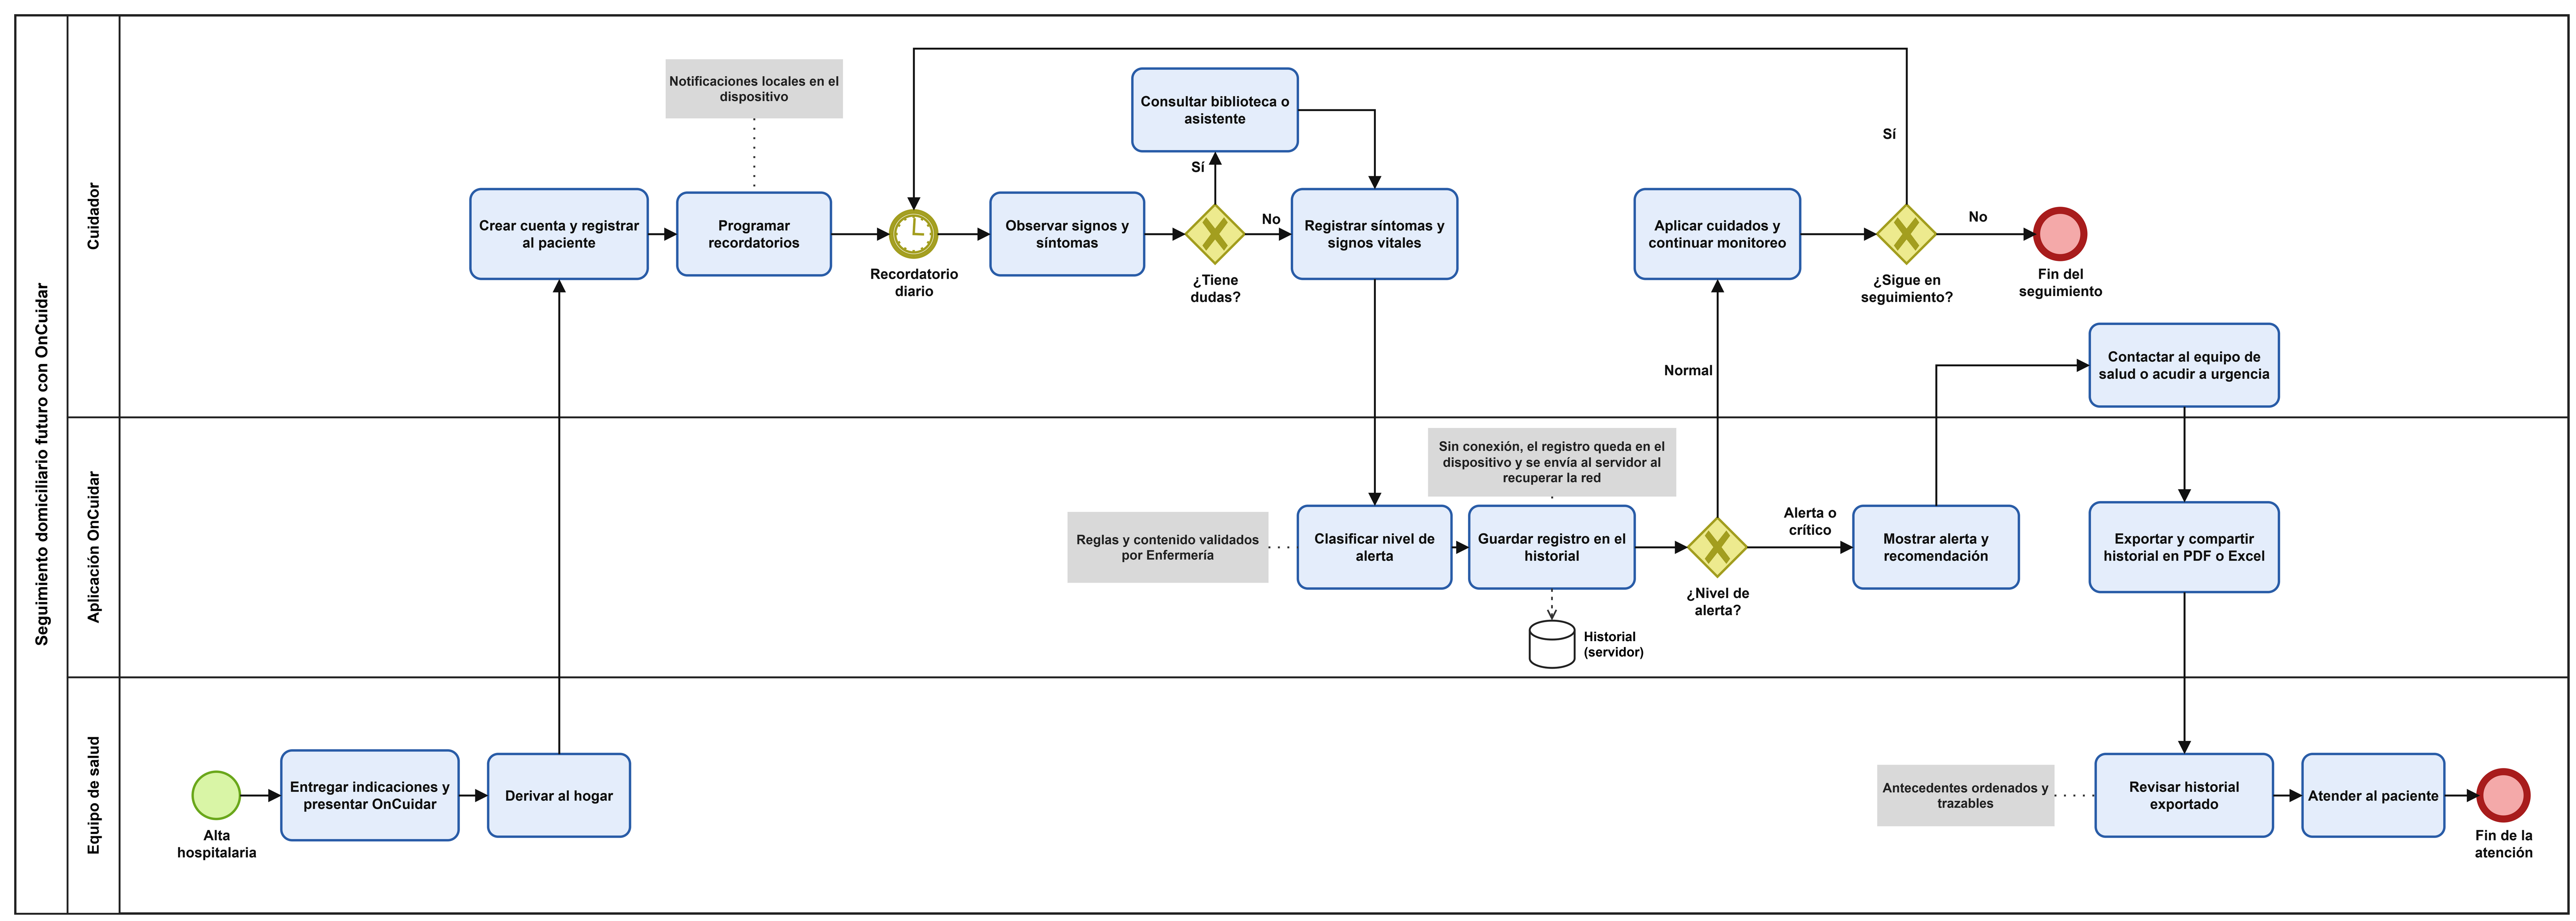
\includegraphics[width=\linewidth, keepaspectratio]{figures/bpmn/bpmn-futuro.png}
    \caption{Proceso de negocio futuro con la aplicación OnCuidar.}
    \label{fig:bpmn-futuro}
\end{figure}
\end{landscape}
\restoregeometry

El proceso comienza con el alta, cuando el equipo de salud entrega las
indicaciones y presenta la aplicación. En el hogar, el cuidador crea su cuenta,
registra al paciente y programa los recordatorios. Cuando suena el recordatorio
diario, observa los signos y síntomas y, si tiene dudas, consulta la biblioteca
o el asistente antes de registrar la valoración. La aplicación clasifica el
nivel de alerta con el motor de reglas y guarda el registro en el historial; sin
conexión, lo conserva en el dispositivo y lo envía al servidor al recuperar la red. Si
el nivel es normal, el cuidador continúa el monitoreo hasta el siguiente
recordatorio. Si es de alerta o crítico, la aplicación muestra la alerta con su
recomendación y el cuidador contacta al equipo de salud o acude a urgencia. En
el control, exporta y comparte el historial en PDF o Excel, y el equipo clínico
revisa antecedentes ordenados en lugar de reconstruirlos desde el relato.

La aplicación no reemplaza la decisión clínica. Su función es acortar el tiempo
entre la aparición de un signo de alerta y el contacto con el equipo de salud, y
mejorar la calidad de la información disponible en cada control.

\section[Diagrama de Flujo de Datos]{Diagrama de flujo de datos}

Según la plantilla, este ítem es excluyente con el diagrama de casos de uso. El
proyecto modela la funcionalidad mediante casos de uso, desarrollados en la
sección siguiente.

\section[Casos de Uso]{Diagrama de casos de uso}

La Figura~\ref{fig:casos-uso} presenta los casos de uso del sistema. Cada
requerimiento funcional del capítulo~4 queda representado por al menos un caso
de uso, como detalla el Anexo de trazabilidad.

\begin{figure}[H]
    \centering
    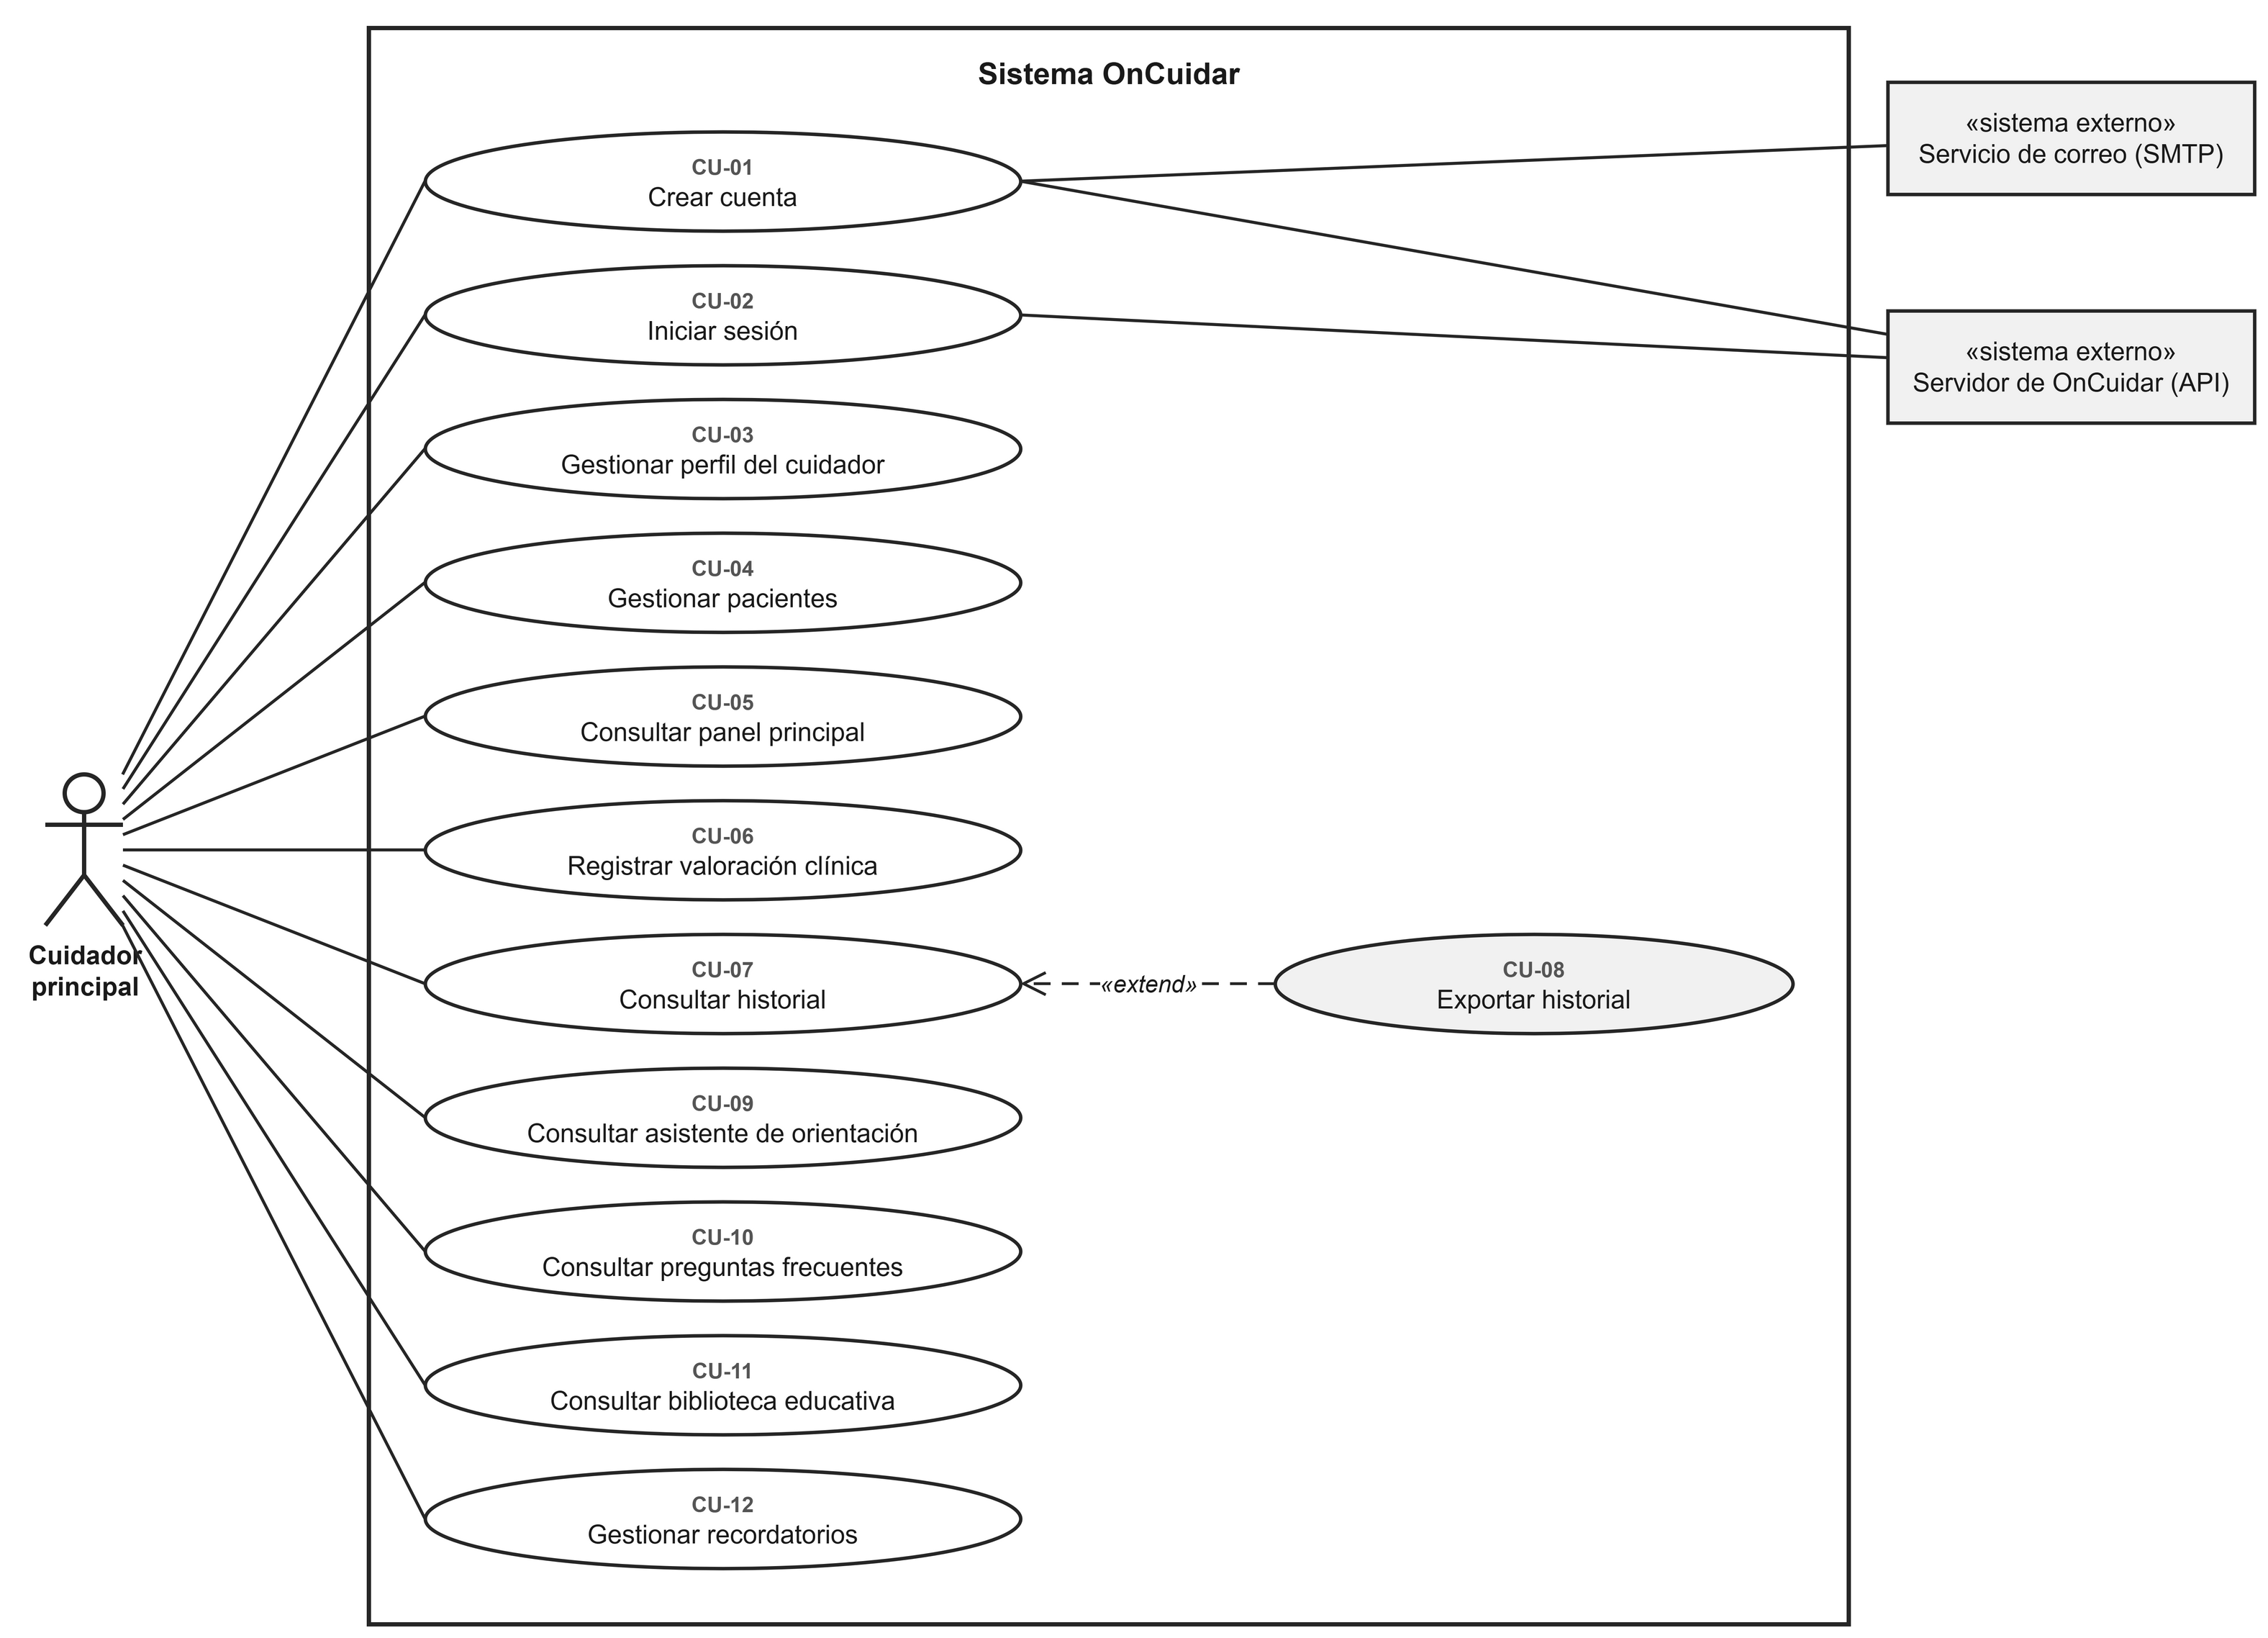
\includegraphics[width=0.92\textwidth, keepaspectratio]{figures/casos-uso/cu-general.png}
    \caption{Diagrama de casos de uso de OnCuidar.}
    \label{fig:casos-uso}
\end{figure}

\subsection[Actores]{Actores}

\begin{table}[H]
\centering
\small
\tablazebra
\caption{Actores del sistema.}
\label{tab:actores}
\begin{tabularx}{\textwidth}{P{0.62}P{1.20}P{0.88}P{1.30}}
\toprule
\filaencabezado \encab{Actor} & \encab{Rol o funciones} & \encab{Conocimientos técnicos} & \encab{Privilegios y funcionalidades} \\
\midrule
Cuidador principal &
Madre, padre o tutor que acompaña al paciente en el hogar, registra su
evolución y aplica las indicaciones del equipo de salud. &
Básicos. Maneja un teléfono inteligente, pero no tiene formación técnica ni
clínica. &
Accede a todas las funciones de la aplicación, limitadas a sus propios datos y a
los de sus pacientes. \\
Servidor de OnCuidar (API) &
Servicio que autentica a los usuarios y almacena los datos de la aplicación en
la base de datos PostgreSQL. Se ejecuta en contenedores, en el servidor de la
Universidad del Bío-Bío. &
No aplica. &
Valida credenciales, entrega al dispositivo la clave de datos del cuidador,
rechaza los datos sensibles en claro y solo permite acceder a los datos del
usuario autenticado. \\
Servicio de correo (SMTP) &
Servicio externo que entrega los correos que envía el servidor. &
No aplica. &
Entrega los enlaces de un solo uso para restablecer la contraseña y confirmar
los correos del cuidador. \\
\bottomrule
\end{tabularx}
\end{table}

\subsection[Diagrama y Descripción]{Casos de uso y descripción}

El cuidador comienza creando una cuenta con sus datos y los de su paciente, y en
los usos siguientes inicia sesión. Desde el perfil puede actualizar sus datos,
agregar otros pacientes y elegir cuál está activo. El panel principal le muestra
el estado del paciente activo y lo lleva a cada módulo.

En su rutina diaria, el cuidador registra la valoración clínica del paciente y
recibe de inmediato su nivel de alerta. Cuando necesita revisar la evolución,
consulta el historial y, antes de un control, lo exporta a PDF o Excel. Si tiene
una duda, puede escribirla al asistente, buscarla en las preguntas frecuentes o
consultar la biblioteca educativa. Para no olvidar tareas, programa
recordatorios. El servidor de OnCuidar participa como
sistema externo en la creación de la cuenta y en el inicio de sesión, y el
servicio de correo, al enviar el enlace que confirma el correo del cuidador o
permite restablecer la contraseña.

\subsection[Especificación de los Casos de Uso]{Especificación de los casos de uso}

Esta sección especifica los cinco casos de uso que concentran el valor del
sistema. Los siete restantes se especifican en el anexo de casos de uso.

\subsubsection{Caso de uso: Registrar valoración clínica}

\begin{figure}[H]
    \centering
    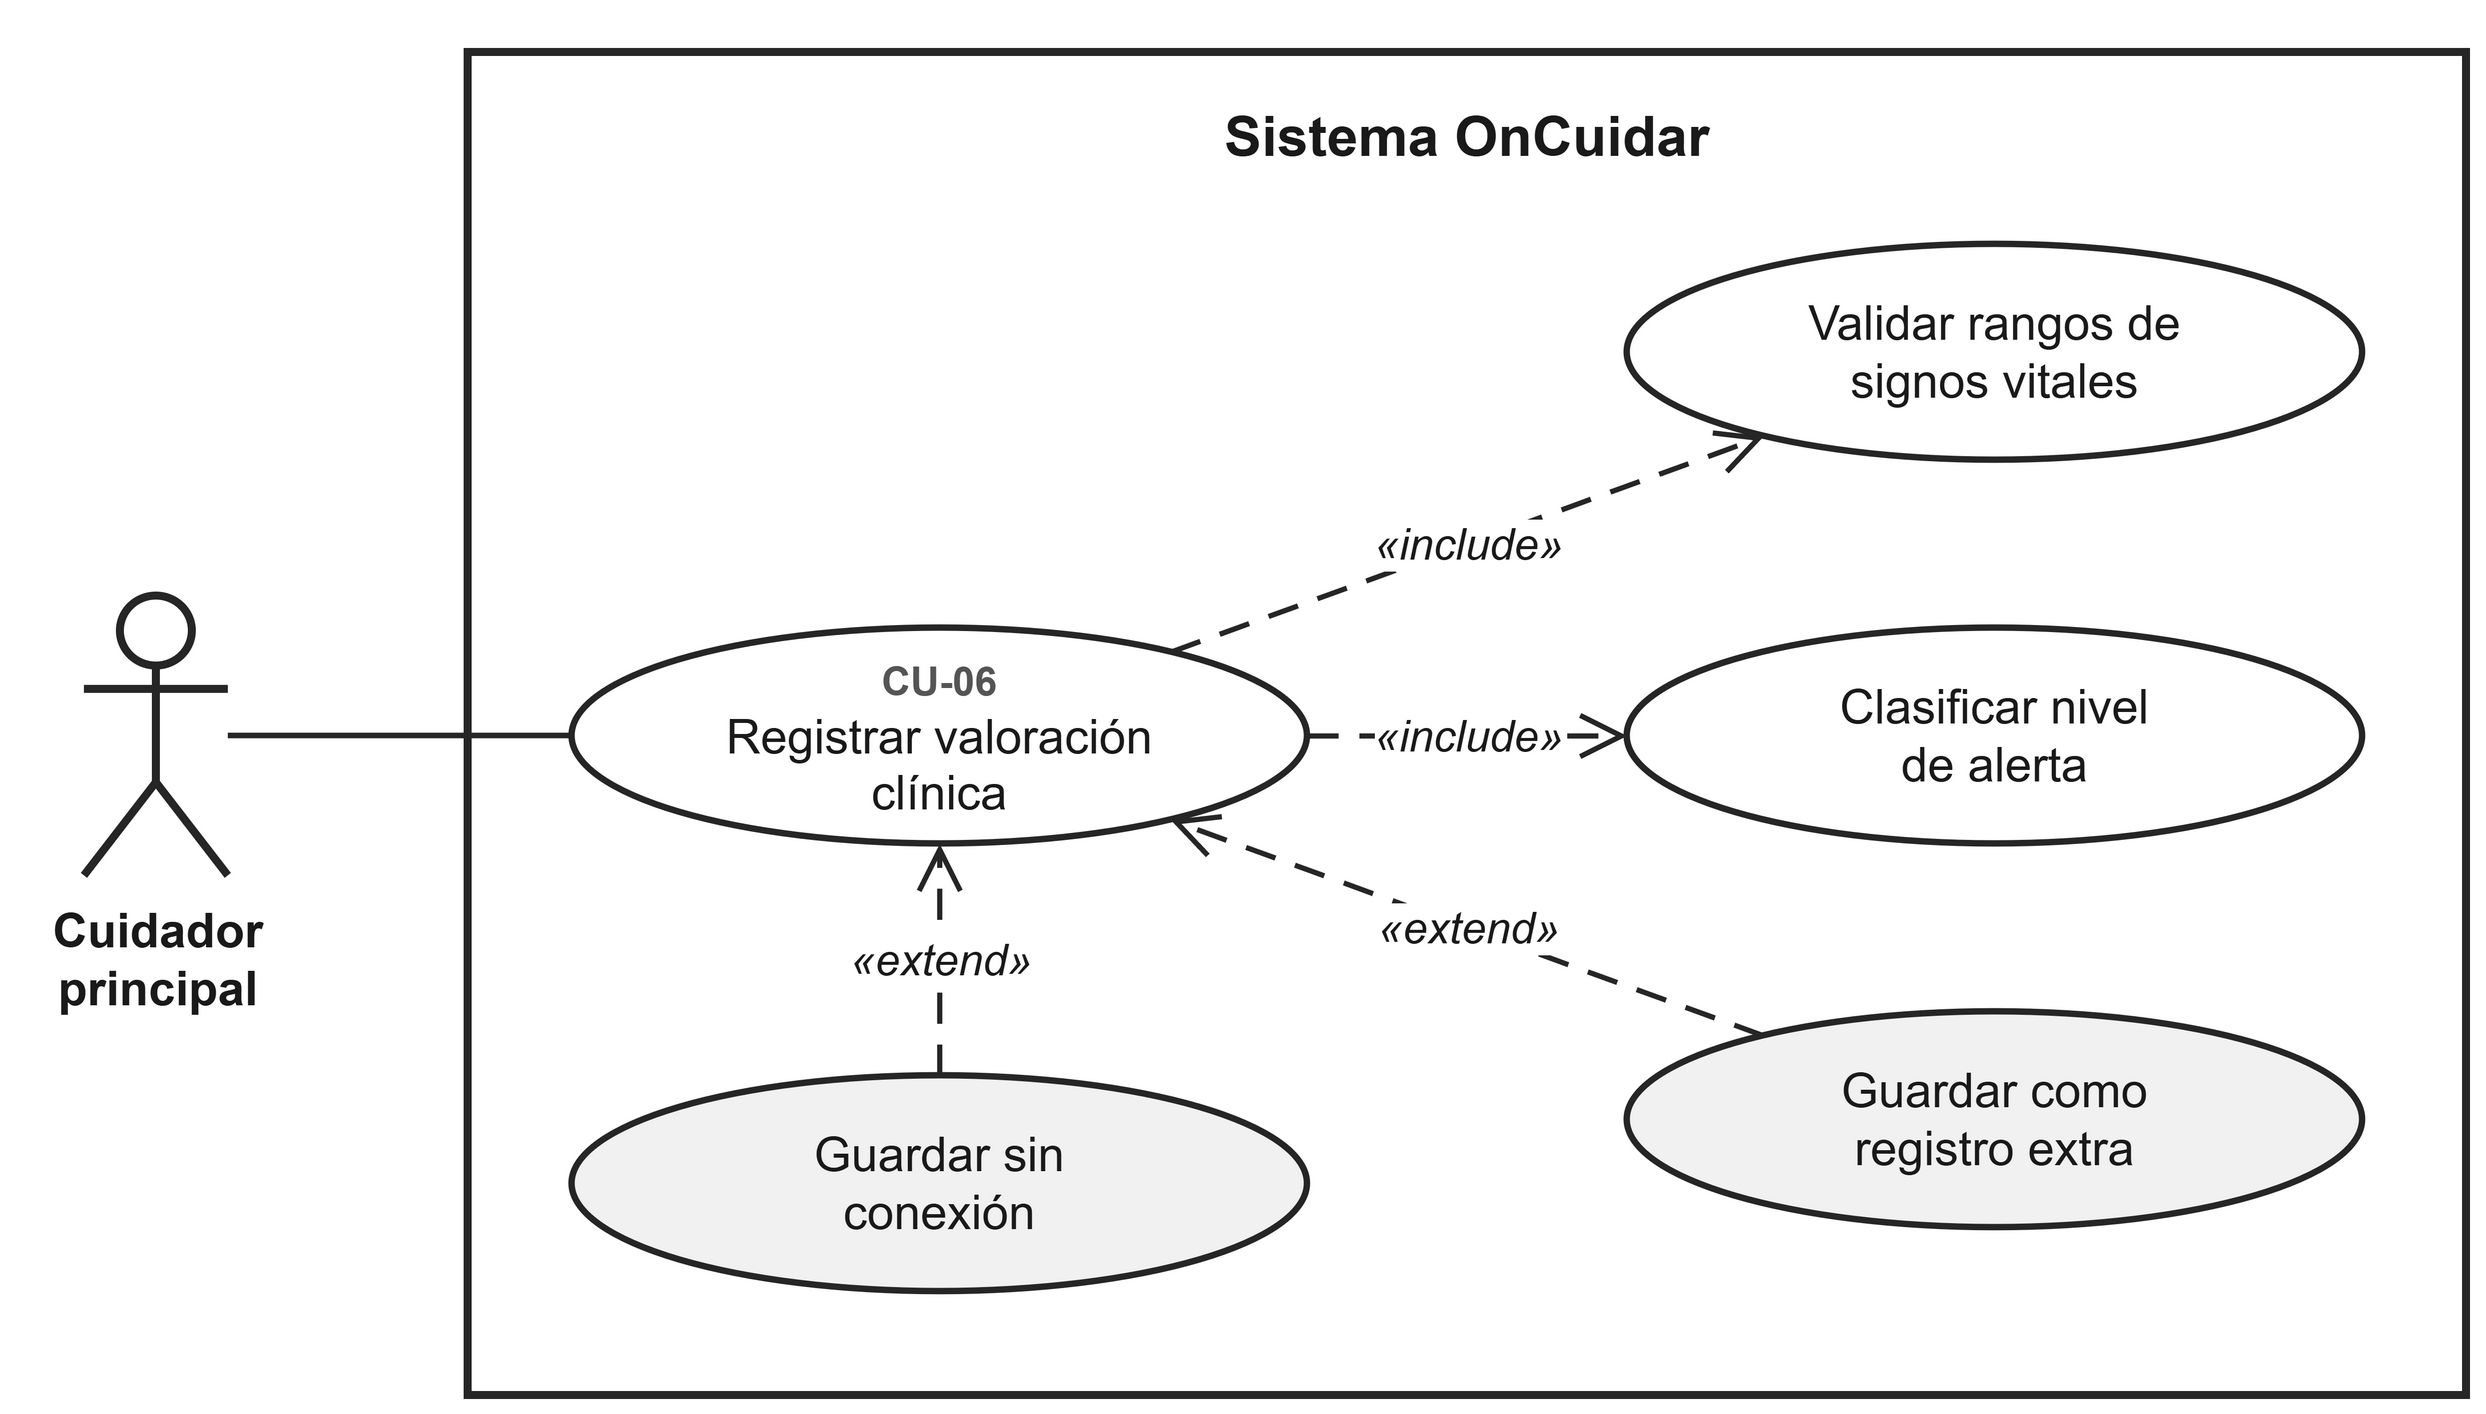
\includegraphics[width=0.9\textwidth, keepaspectratio]{figures/casos-uso/cu-06-registrar-valoracion.png}
    \caption{Diagrama del caso de uso CU-06: registrar valoración clínica.}
    \label{fig:cu-06}
\end{figure}

\begin{table}[H]
\centering
\caption{Especificación del caso de uso CU-06.}
\label{tab:cu-06}
\begin{especificacioncu}{CU-06}{Registrar valoración clínica}
    \cufila{Descripción}{El cuidador registra los signos vitales, los síntomas y
    las observaciones del paciente activo, y el sistema clasifica el nivel de
    alerta del registro.}
    \cufila{Actor}{Cuidador principal.}
    \cufila{Requerimientos}{RF-11, RF-12, RF-13, RF-28.}
    \cufila{Precondiciones}{El cuidador inició sesión y tiene un paciente
    activo.}
    \cuflujo{Flujo de eventos básico}
    \cupaso{1. Selecciona Registro en la barra inferior.}
           {2. Muestra el formulario con el tipo de registro, los signos
           vitales, los síntomas ESAS y las observaciones.}
    \cupaso{3. Ingresa los signos vitales que conoce, la intensidad de cada
           síntoma y, si lo desea, observaciones.}
           {4. Valida que cada signo esté dentro de su rango físico y muestra
           el nivel de alerta calculado.}
    \cupaso{5. Presiona Guardar.}
           {6. Cifra los datos sensibles, guarda el registro con fecha y hora y
           confirma el guardado.}
    \cupaso{}{7. Muestra el nivel de alerta, los motivos detectados y la
           recomendación correspondiente.}
    \cufinflujo
    \cuflujo{Flujos alternativos}
    \cupaso{}{4a. Si un signo está fuera de rango, indica el rango permitido y
           no permite guardar hasta que se corrija.}
    \cupaso{}{6a. Si el paciente alcanzó su tope diario de registros
           programados, guarda el registro como extra.}
    \cupaso{}{6b. Si no hay conexión, guarda el registro en el dispositivo y lo
           lo envía al servidor al recuperar la red.}
    \cufinflujo
    \cufila{Postcondiciones}{El registro queda en el historial del paciente con
    su nivel de alerta y el panel principal se actualiza.}
\end{especificacioncu}
\end{table}

\subsubsection{Caso de uso: Exportar historial}

\begin{figure}[H]
    \centering
    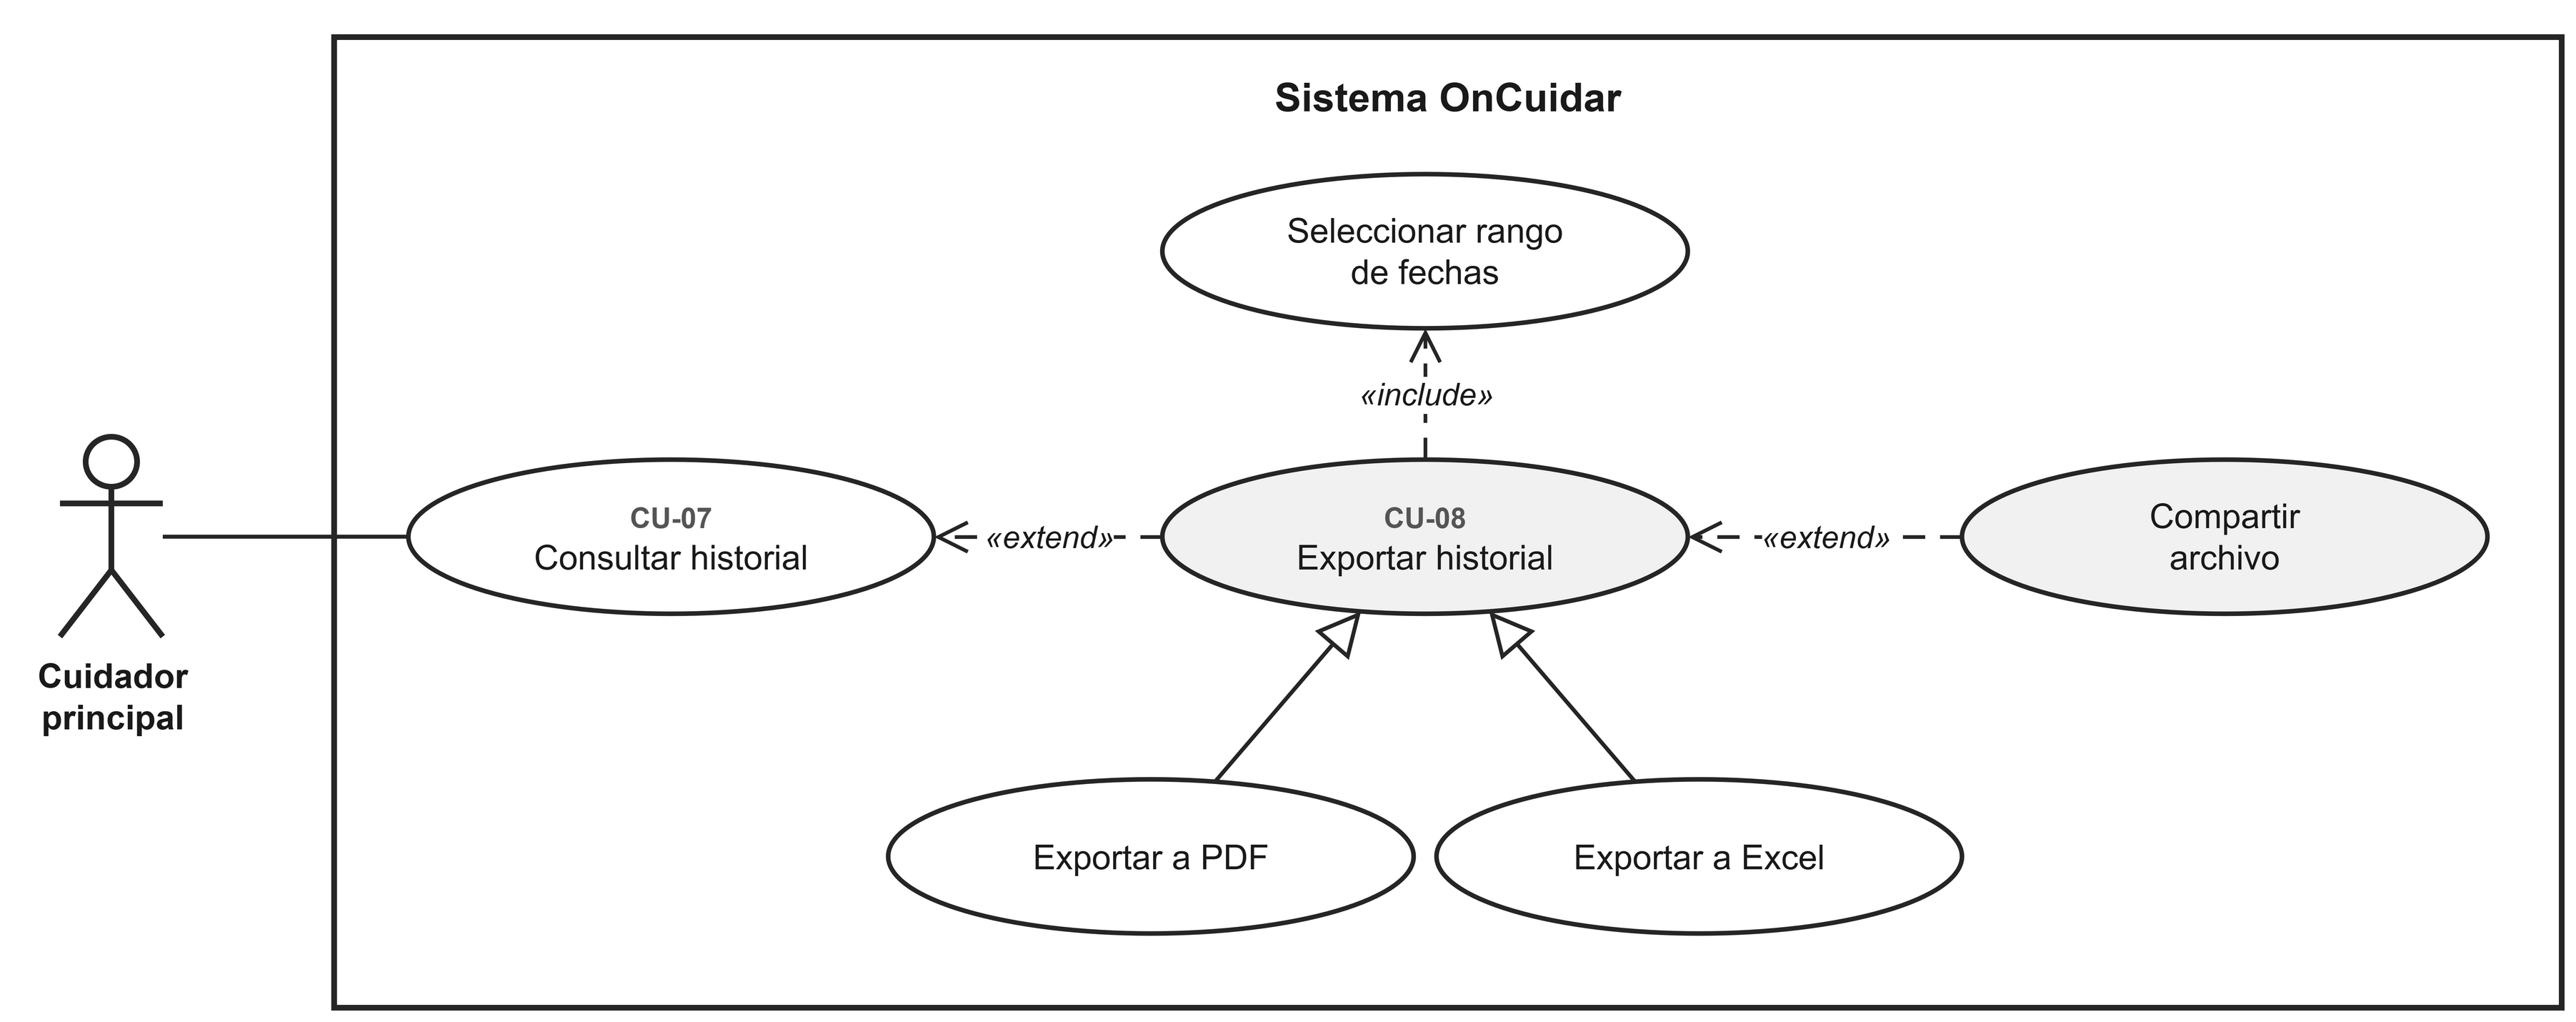
\includegraphics[width=0.9\textwidth, keepaspectratio]{figures/casos-uso/cu-08-exportar-historial.png}
    \caption{Diagrama del caso de uso CU-08: exportar historial.}
    \label{fig:cu-08}
\end{figure}

\begin{table}[H]
\centering
\caption{Especificación del caso de uso CU-08.}
\label{tab:cu-08}
\begin{especificacioncu}{CU-08}{Exportar historial}
    \cufila{Descripción}{El cuidador genera un informe del historial del paciente
    activo en PDF o Excel para presentarlo en un control clínico.}
    \cufila{Actor}{Cuidador principal.}
    \cufila{Requerimientos}{RF-16, RF-17.}
    \cufila{Precondiciones}{El paciente activo tiene registros en el historial.}
    \cuflujo{Flujo de eventos básico}
    \cupaso{1. Desde el historial, elige exportar y selecciona PDF o Excel.}
           {2. Solicita el rango de fechas del informe.}
    \cupaso{3. Indica el rango de fechas.}
           {4. Descifra los registros del rango y genera el archivo con los
           datos del paciente, del cuidador, del centro de salud y del contacto
           de emergencia, junto con el detalle de cada registro.}
    \cupaso{}{5. Guarda el archivo en el dispositivo y ofrece abrirlo o
           compartirlo.}
    \cupaso{6. Abre el archivo o lo comparte.}{}
    \cufinflujo
    \cuflujo{Flujos alternativos}
    \cupaso{}{4a. Si no hay registros en el rango elegido, informa que no hay
           datos para exportar.}
    \cufinflujo
    \cufila{Postcondiciones}{El informe queda guardado en el dispositivo del
    cuidador.}
\end{especificacioncu}
\end{table}

\subsubsection{Caso de uso: Consultar asistente de orientación}

\begin{figure}[H]
    \centering
    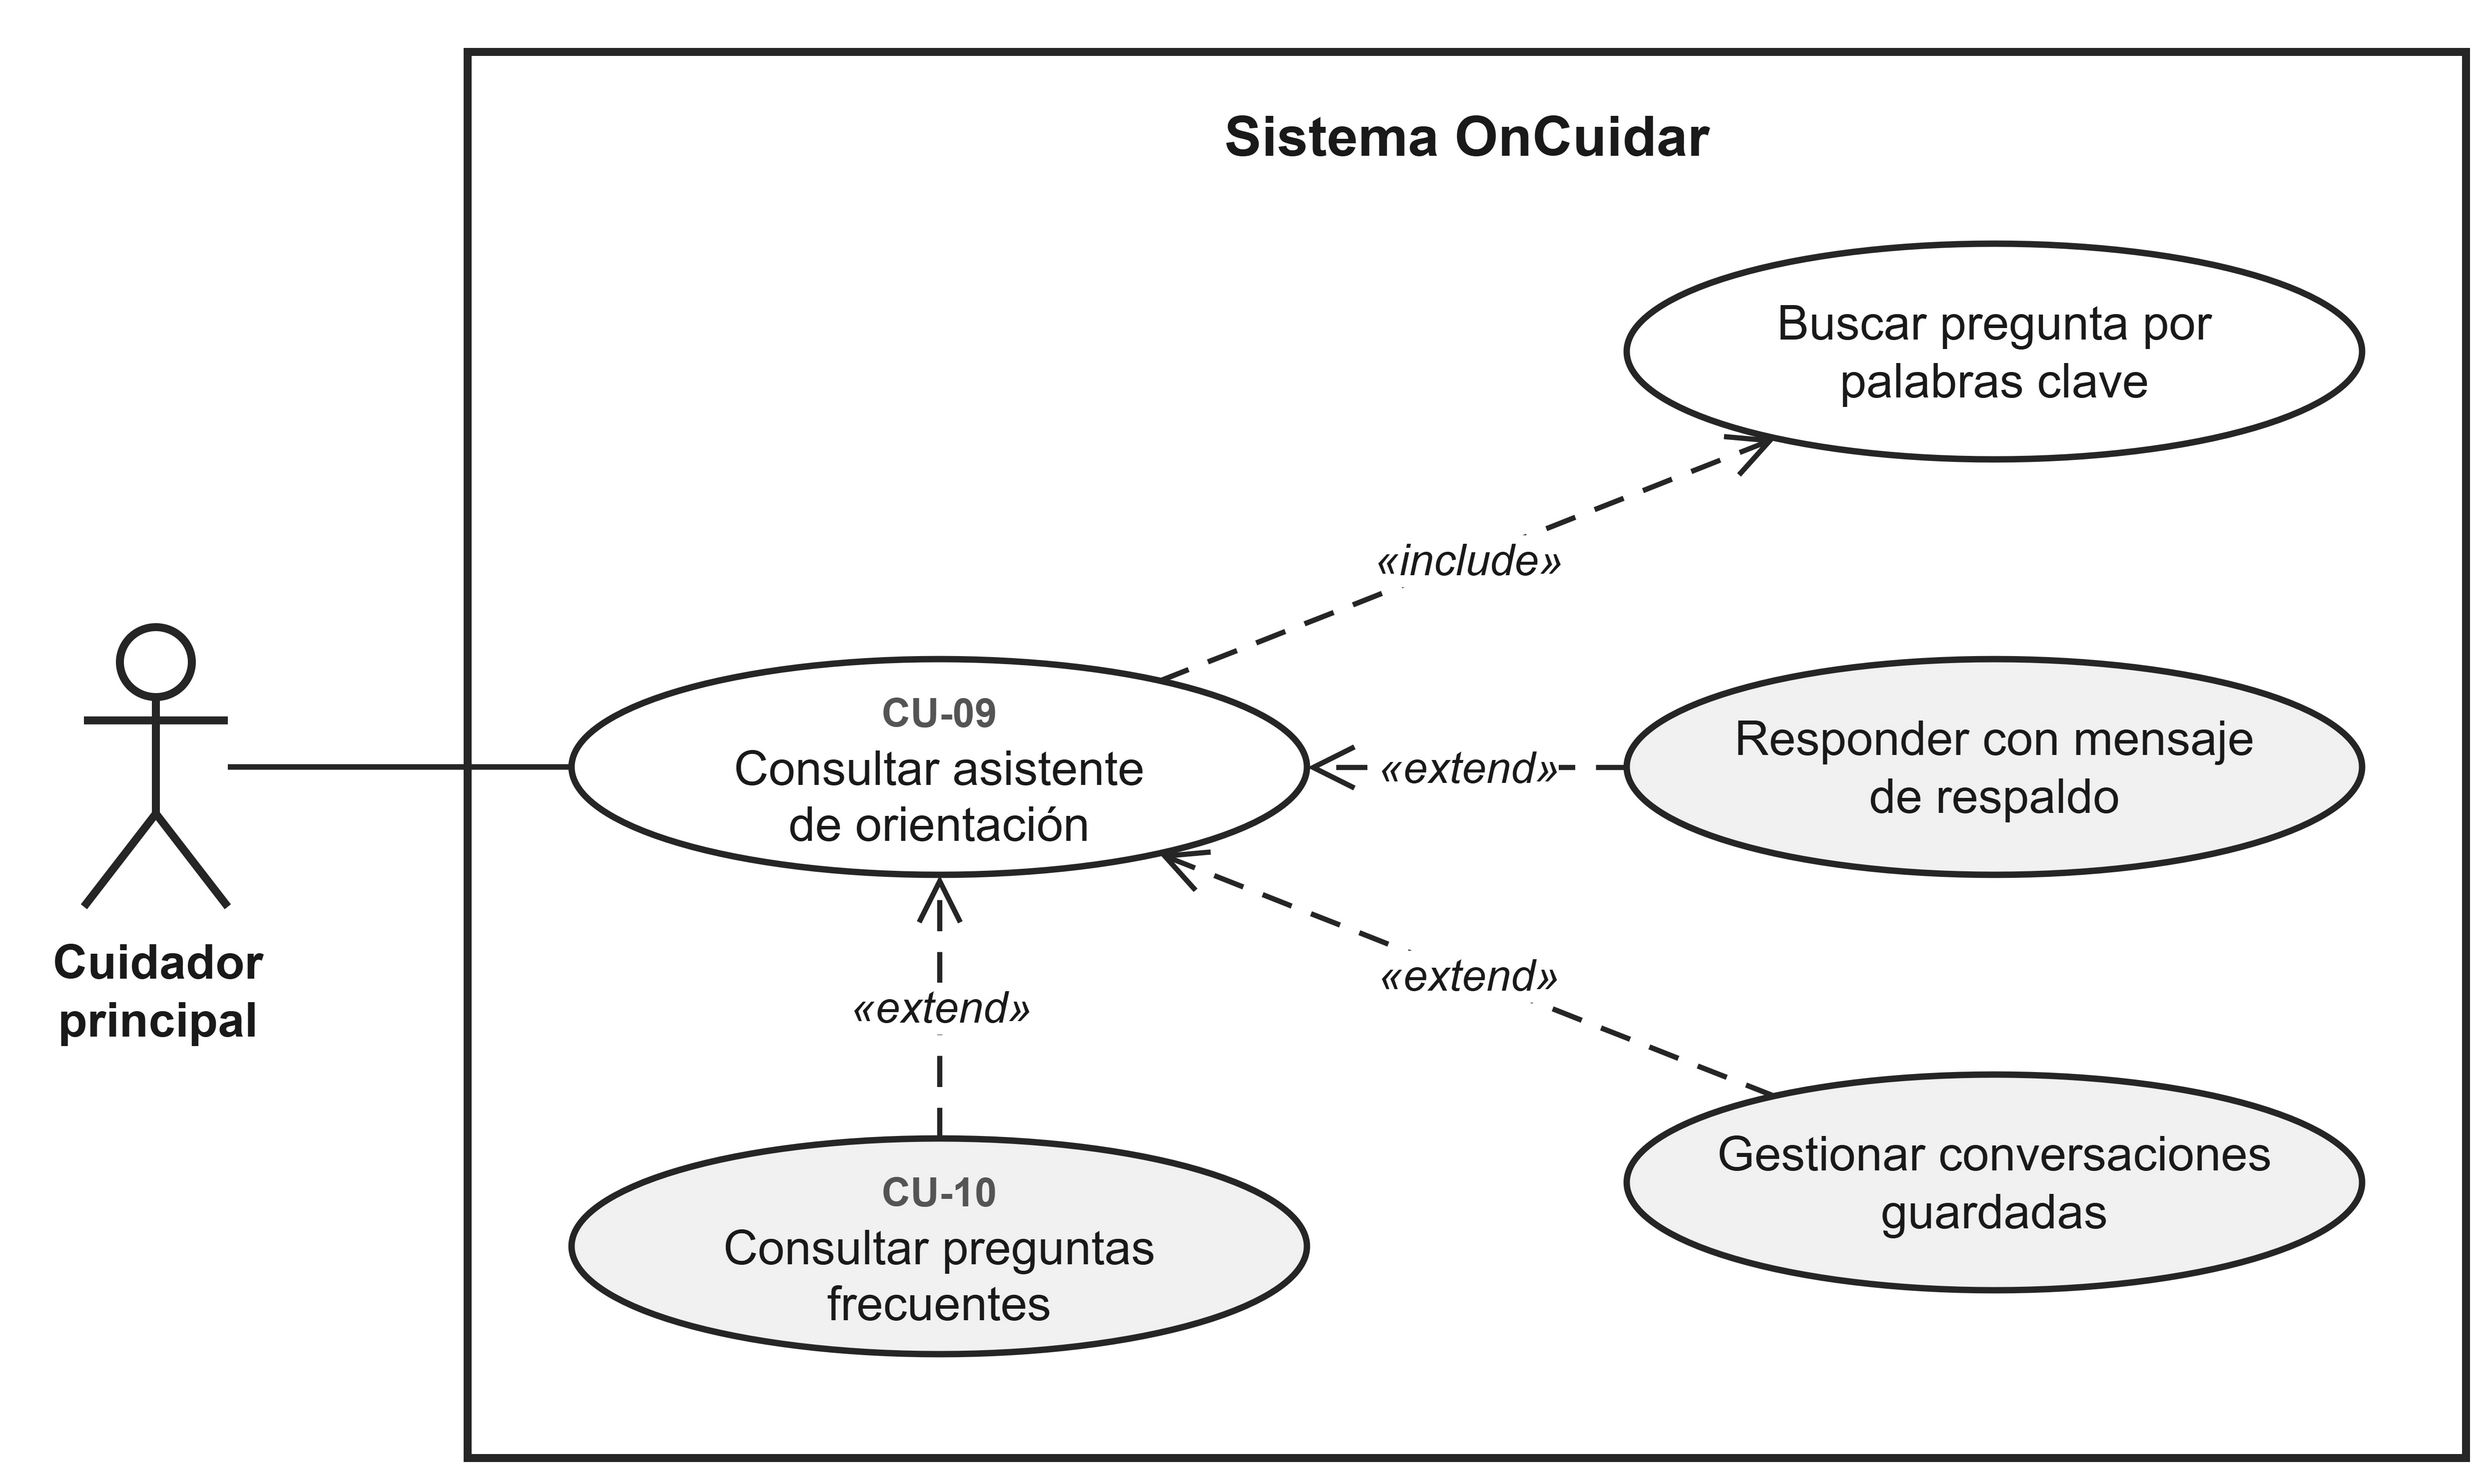
\includegraphics[width=0.9\textwidth, keepaspectratio]{figures/casos-uso/cu-09-asistente.png}
    \caption{Diagrama del caso de uso CU-09: consultar asistente de orientación.}
    \label{fig:cu-09}
\end{figure}

\begin{table}[H]
\centering
\caption{Especificación del caso de uso CU-09.}
\label{tab:cu-09}
\begin{especificacioncu}{CU-09}{Consultar asistente de orientación}
    \cufila{Descripción}{El cuidador escribe una duda y recibe la respuesta de la
    pregunta frecuente validada que mejor coincide con ella.}
    \cufila{Actor}{Cuidador principal.}
    \cufila{Requerimientos}{RF-19, RF-20.}
    \cufila{Precondiciones}{El cuidador inició sesión.}
    \cuflujo{Flujo de eventos básico}
    \cupaso{1. Selecciona Chat en la barra inferior.}
           {2. Muestra un mensaje de bienvenida y preguntas sugeridas.}
    \cupaso{3. Escribe su consulta o elige una pregunta sugerida.}
           {4. Busca la pregunta frecuente que comparte más palabras clave con
           la consulta.}
    \cupaso{}{5. Muestra la respuesta validada y guarda la conversación con un
           título automático.}
    \cupaso{6. Continúa la conversación o sale del chat.}{}
    \cufinflujo
    \cuflujo{Flujos alternativos}
    \cupaso{}{4a. Si ninguna pregunta alcanza la coincidencia mínima, responde
           que aún no tiene una respuesta exacta, sugiere los temas disponibles y
           recomienda consultar al equipo médico.}
    \cupaso{1a. Abre sus conversaciones guardadas.}
           {1b. Las lista por última actividad y permite continuarlas,
           renombrarlas o eliminarlas.}
    \cufinflujo
    \cufila{Postcondiciones}{La conversación queda guardada en la cuenta del
    cuidador, con sus mensajes cifrados.}
\end{especificacioncu}
\end{table}

\subsubsection{Caso de uso: Consultar biblioteca educativa}

\begin{figure}[H]
    \centering
    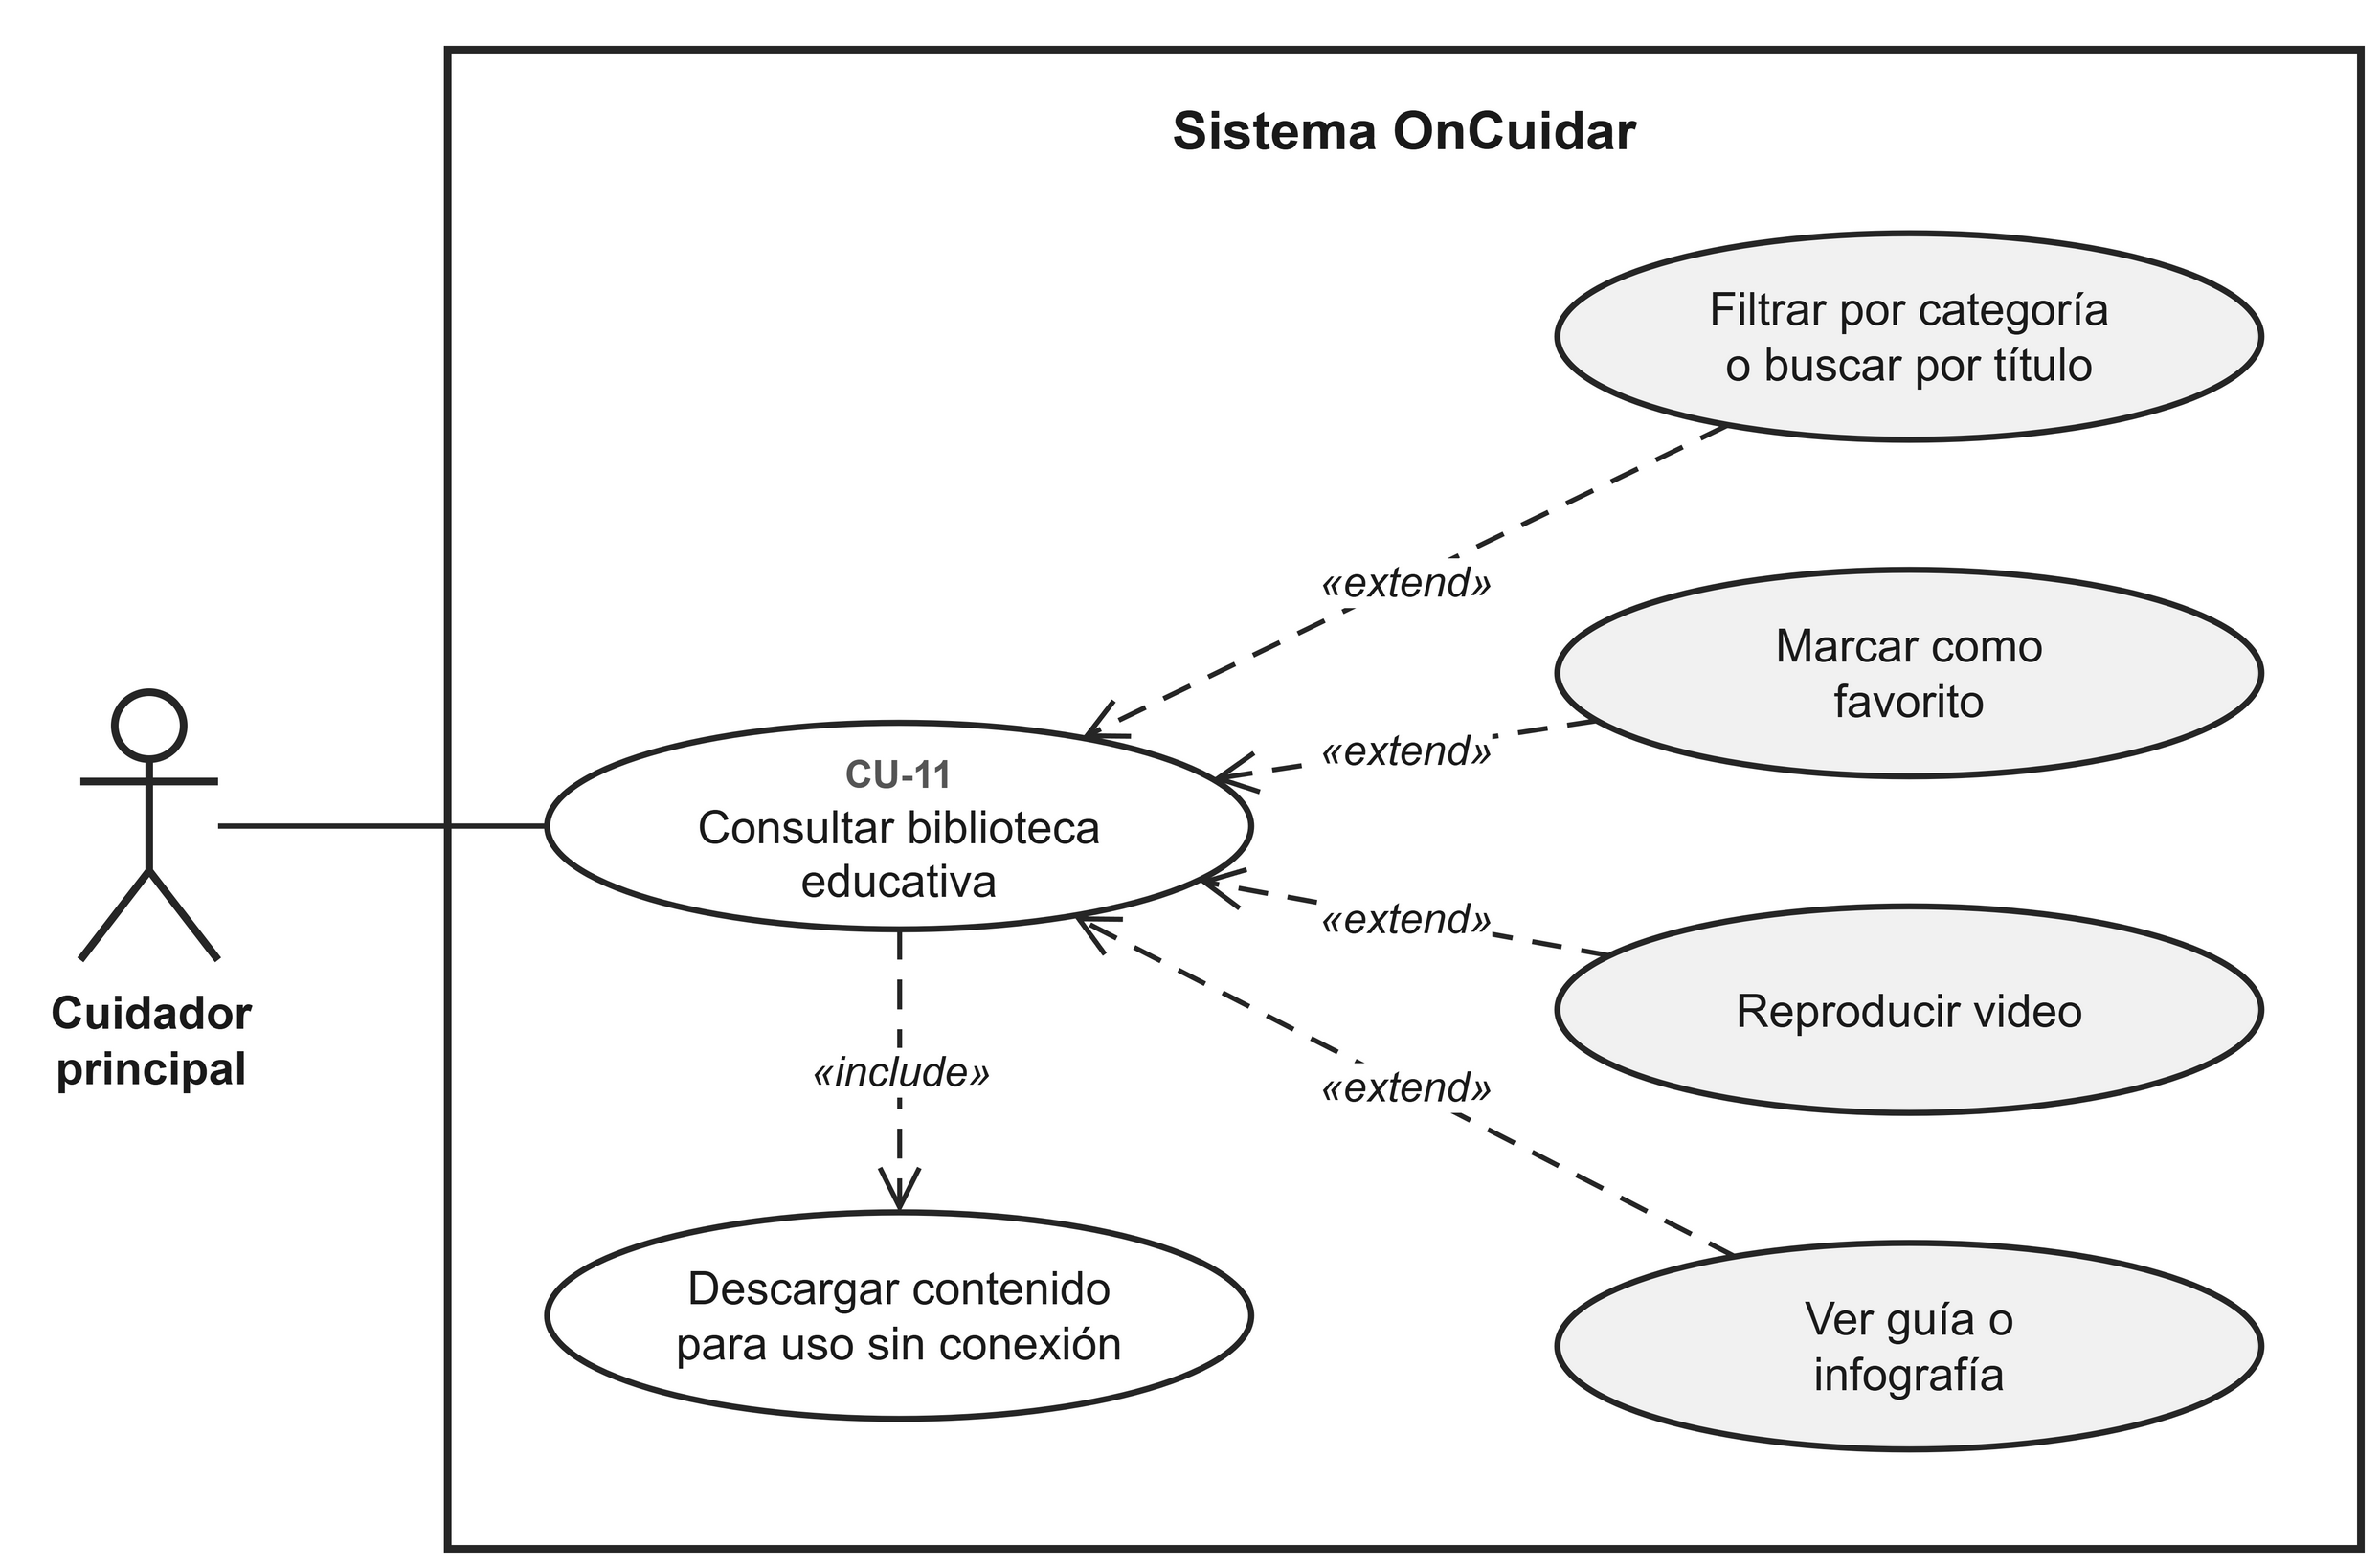
\includegraphics[width=0.9\textwidth, keepaspectratio]{figures/casos-uso/cu-11-biblioteca.png}
    \caption{Diagrama del caso de uso CU-11: consultar biblioteca educativa.}
    \label{fig:cu-11}
\end{figure}

\begin{table}[H]
\centering
\caption{Especificación del caso de uso CU-11.}
\label{tab:cu-11}
\begin{especificacioncu}{CU-11}{Consultar biblioteca educativa}
    \cufila{Descripción}{El cuidador consulta videos, guías, infografías y
    documentos validados por Enfermería, incluso sin conexión.}
    \cufila{Actor}{Cuidador principal.}
    \cufila{Requerimientos}{RF-24, RF-25, RF-26, RF-27.}
    \cufila{Precondiciones}{El cuidador inició sesión y el contenido educativo
    está publicado.}
    \cuflujo{Flujo de eventos básico}
    \cupaso{1. Selecciona Aprende en la barra inferior.}
           {2. Muestra el catálogo con la categoría, el tipo y el estado de
           descarga de cada material.}
    \cupaso{3. Filtra por categoría o busca por título.}
           {4. Muestra los materiales que coinciden.}
    \cupaso{5. Abre un material.}
           {6. Presenta el material según su tipo: reproduce el video, muestra la
           guía o amplía la infografía.}
    \cupaso{7. Marca el material como favorito.}
           {8. Guarda el favorito en la cuenta del cuidador.}
    \cufinflujo
    \cuflujo{Flujos alternativos}
    \cupaso{}{4a. Si no hay coincidencias, informa que no se encontraron
           materiales.}
    \cupaso{}{6a. Si no hay conexión, abre el material desde la copia
           descargada en el dispositivo.}
    \cufinflujo
    \cufila{Postcondiciones}{Los favoritos quedan guardados en la cuenta del
    cuidador.}
\end{especificacioncu}
\end{table}

\subsubsection{Caso de uso: Gestionar recordatorios}

\begin{figure}[H]
    \centering
    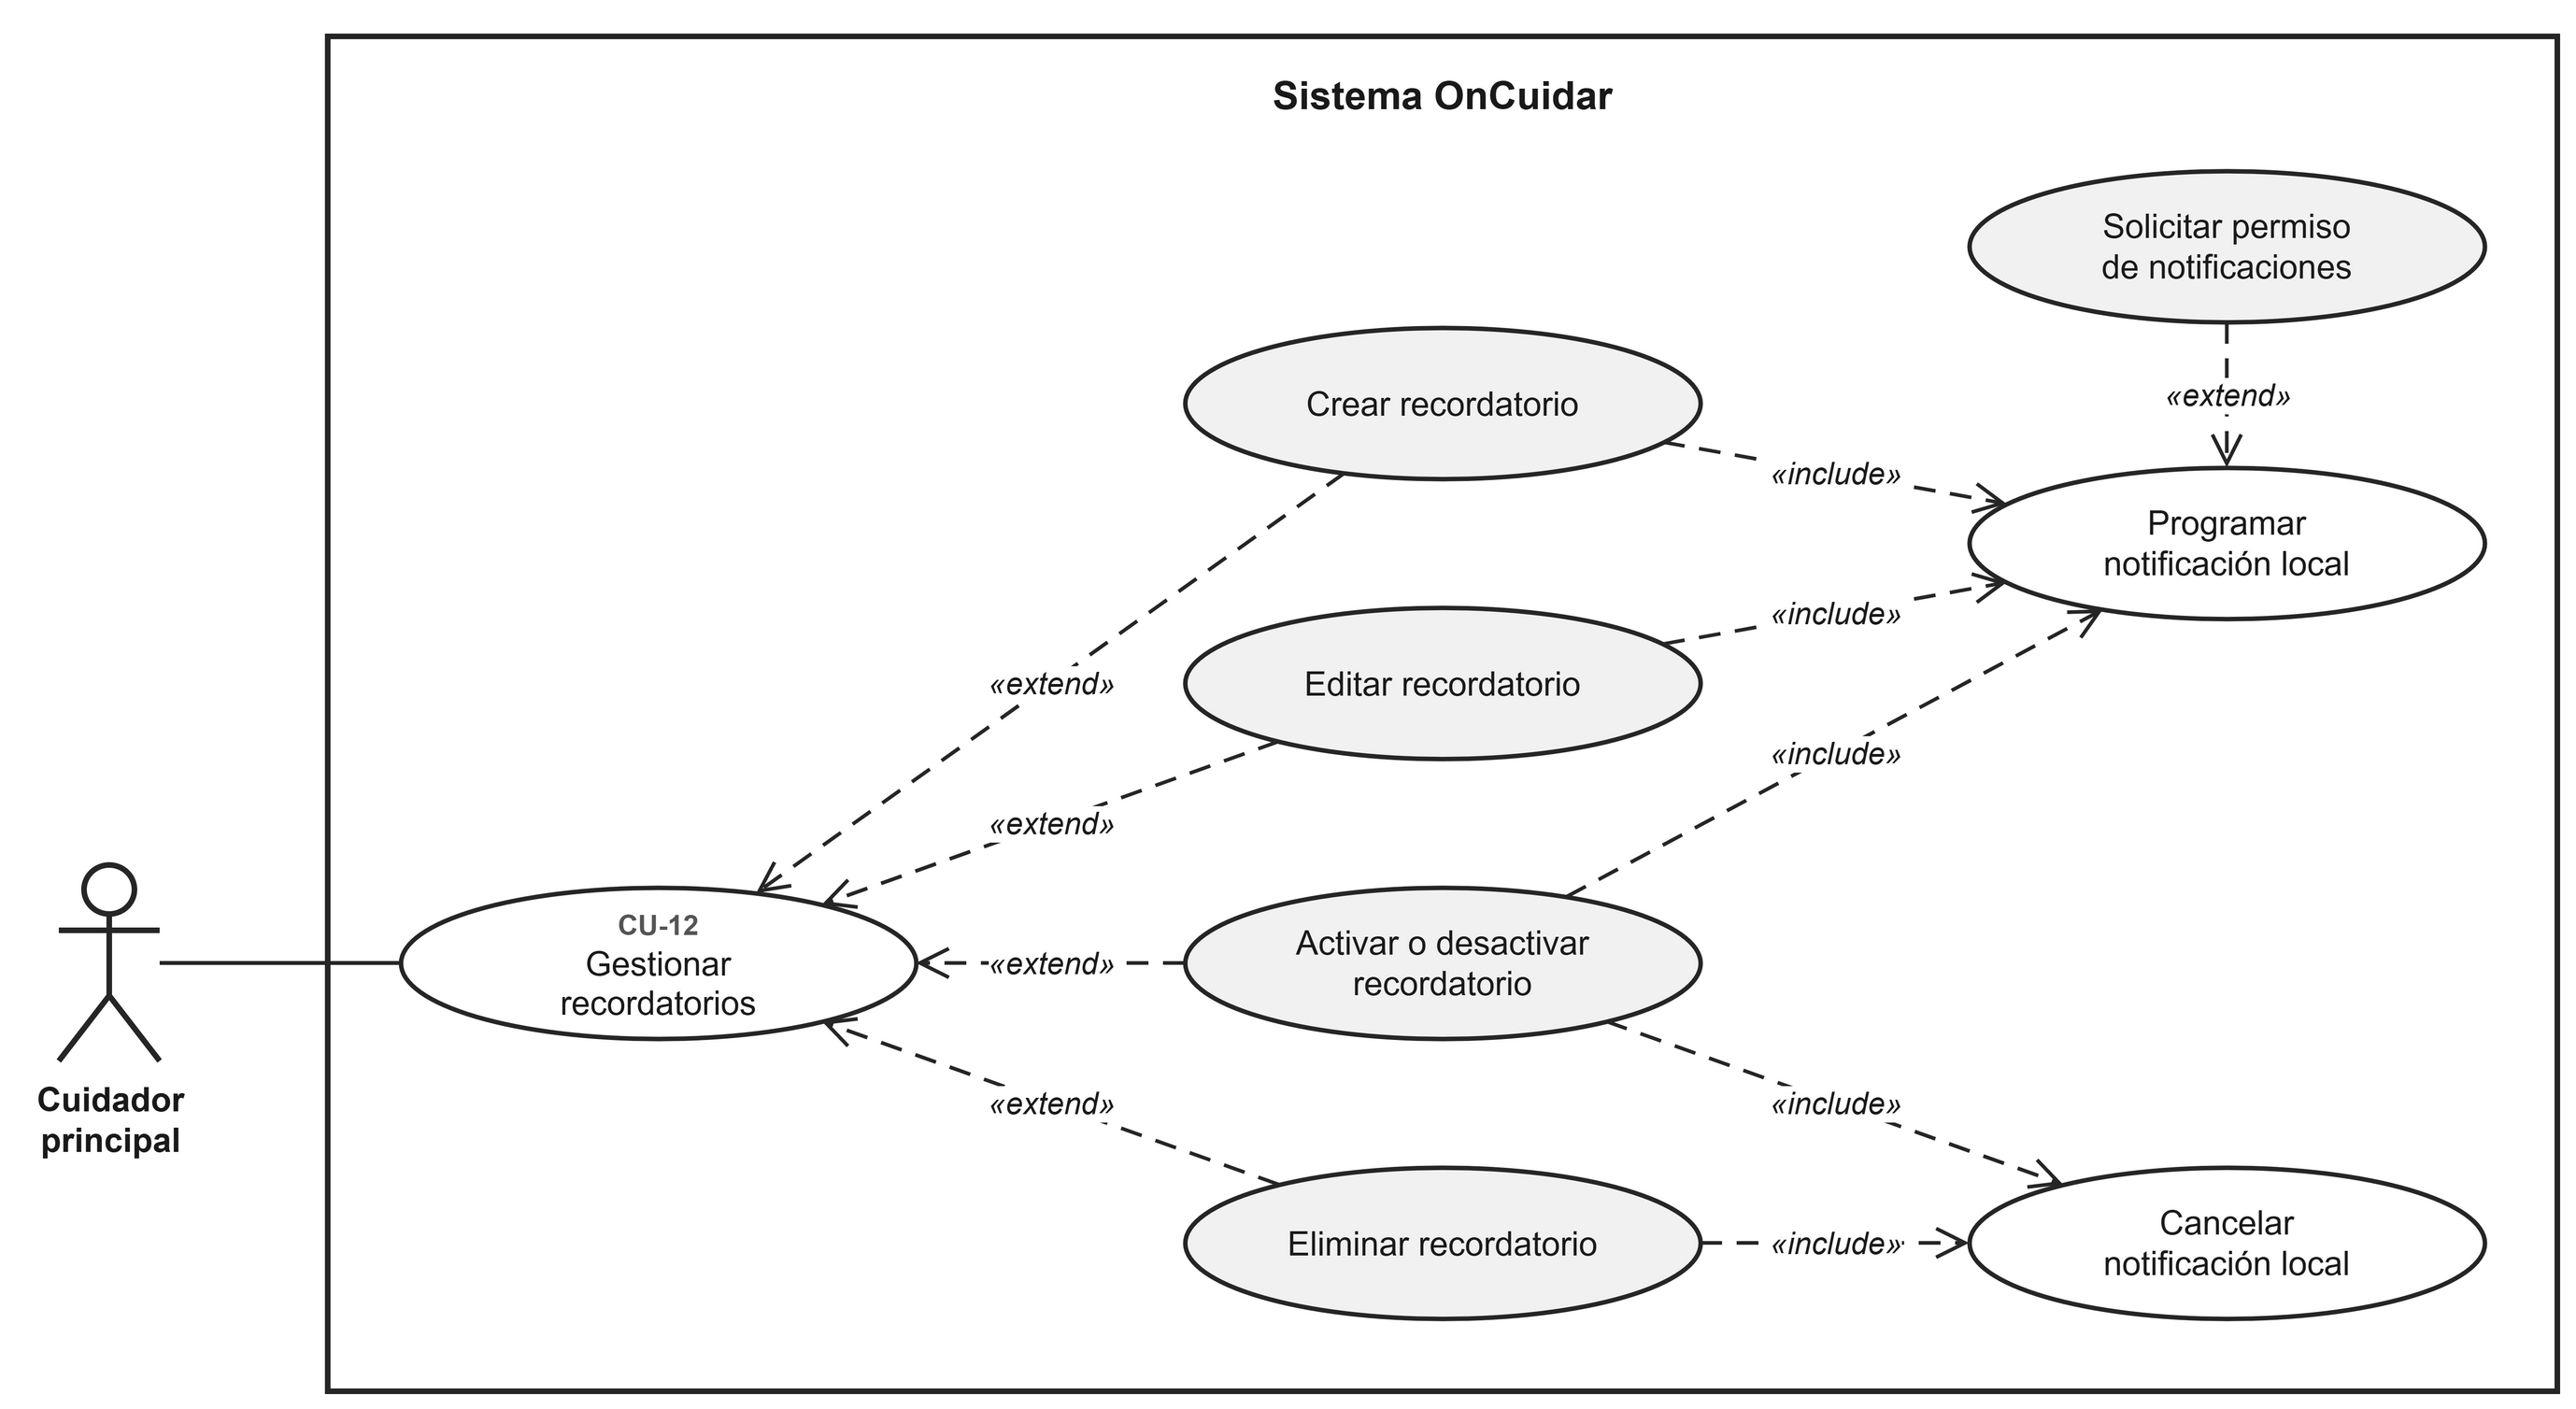
\includegraphics[width=0.9\textwidth, keepaspectratio]{figures/casos-uso/cu-12-recordatorios.png}
    \caption{Diagrama del caso de uso CU-12: gestionar recordatorios.}
    \label{fig:cu-12}
\end{figure}

\begin{table}[H]
\centering
\caption{Especificación del caso de uso CU-12.}
\label{tab:cu-12}
\begin{especificacioncu}{CU-12}{Gestionar recordatorios}
    \cufila{Descripción}{El cuidador programa recordatorios de medicamentos,
    mediciones, citas u otras tareas del paciente activo y recibe una
    notificación a la hora indicada.}
    \cufila{Actor}{Cuidador principal.}
    \cufila{Requerimientos}{RF-22, RF-23.}
    \cufila{Precondiciones}{El cuidador inició sesión y tiene un paciente
    activo.}
    \cuflujo{Flujo de eventos básico}
    \cupaso{1. Abre Recordatorios desde el panel principal.}
           {2. Lista los recordatorios del paciente activo.}
    \cupaso{3. Crea un recordatorio con título, descripción, tipo, fecha, hora
           y repetición.}
           {4. Valida los datos, guarda el recordatorio y programa la
           notificación local.}
    \cupaso{}{5. A la hora programada, muestra la notificación en el
           dispositivo.}
    \cupaso{6. Desactiva o reactiva un recordatorio con su interruptor.}
           {7. Cancela su notificación al desactivarlo o la vuelve a programar al
           reactivarlo, sin borrar el recordatorio.}
    \cufinflujo
    \cuflujo{Flujos alternativos}
    \cupaso{3a. Edita un recordatorio existente.}
           {3b. Guarda los cambios y reprograma la notificación.}
    \cupaso{3c. Elimina un recordatorio.}
           {3d. Pide confirmación y cancela la notificación programada.}
    \cupaso{}{4a. Si es el primer recordatorio, solicita el permiso de
           notificaciones del dispositivo.}
    \cufinflujo
    \cufila{Postcondiciones}{El recordatorio queda guardado y su notificación
    programada en el dispositivo.}
\end{especificacioncu}
\end{table}

\section[Modelamiento de Datos]{Modelamiento de datos}

El modelo de datos representa la información que gestiona OnCuidar. El cuidador
atiende a uno o más pacientes, inicia conversaciones con el asistente y marca
material educativo como favorito. Es también quien programa los
recordatorios: el paciente no usa la aplicación ni opera ese módulo. Cada
paciente posee registros clínicos, y cada registro clínico incluye síntomas del
catálogo ESAS, y la intensidad y la nota de cada síntoma son
atributos de esa relación. El mensaje es una entidad débil, porque solo existe
dentro de su conversación y se identifica por su orden en ella. La
Tabla~\ref{tab:entidades-mer} resume las entidades y la
Figura~\ref{fig:modelo-datos} presenta el modelo entidad-relación en notación de
Chen, con la cardinalidad de cada relación indicada como 1, N o M. Los signos
vitales son un atributo compuesto, el nivel de alerta es un atributo derivado,
porque lo calcula el motor de reglas clínicas, y los días de repetición de un
recordatorio son multivaluados. Los atributos completos de cada entidad se detallan en el anexo de
diccionario de datos.

\begin{table}[H]
\centering
\small
\tablazebra
\caption{Entidades y relaciones del modelo de datos.}
\label{tab:entidades-mer}
\begin{tabularx}{\textwidth}{P{0.95}P{1.45}P{1.00}P{0.60}}
\toprule
\filaencabezado \encab{Entidad} & \encab{Propósito} & \encab{Relación} & \encab{Cardinalidad} \\
\midrule
Cuidador & Usuario responsable del seguimiento. & Atiende a Paciente & 1:N \\
Paciente & Niño, niña o adolescente en seguimiento, con su centro de salud y contacto de emergencia. & Posee Registro clínico & 1:N \\
Registro clínico & Valoración fechada con signos vitales y nivel de alerta. & Incluye Síntoma & N:M \\
Síntoma & Catálogo de síntomas de la escala ESAS. & Incluido en Registro clínico & N:M \\
Recordatorio & Aviso que el cuidador programa sobre un paciente, dirigido al paciente o al propio cuidador. & Cuidador programa Recordatorio & 1:N \\
Conversación & Consulta al asistente con su título. & Contiene Mensaje & 1:N \\
Mensaje & Entidad débil con cada pregunta o respuesta. & Pertenece a Conversación & N:1 \\
Material educativo & Contenido de la biblioteca validado por Enfermería. & Cuidador marca como favorito Material educativo & N:M \\
\bottomrule
\end{tabularx}
\end{table}

\newgeometry{left=2cm, right=2cm, top=0.8cm, bottom=0.8cm}
\begin{landscape}
\begin{figure}[p]
    \centering
    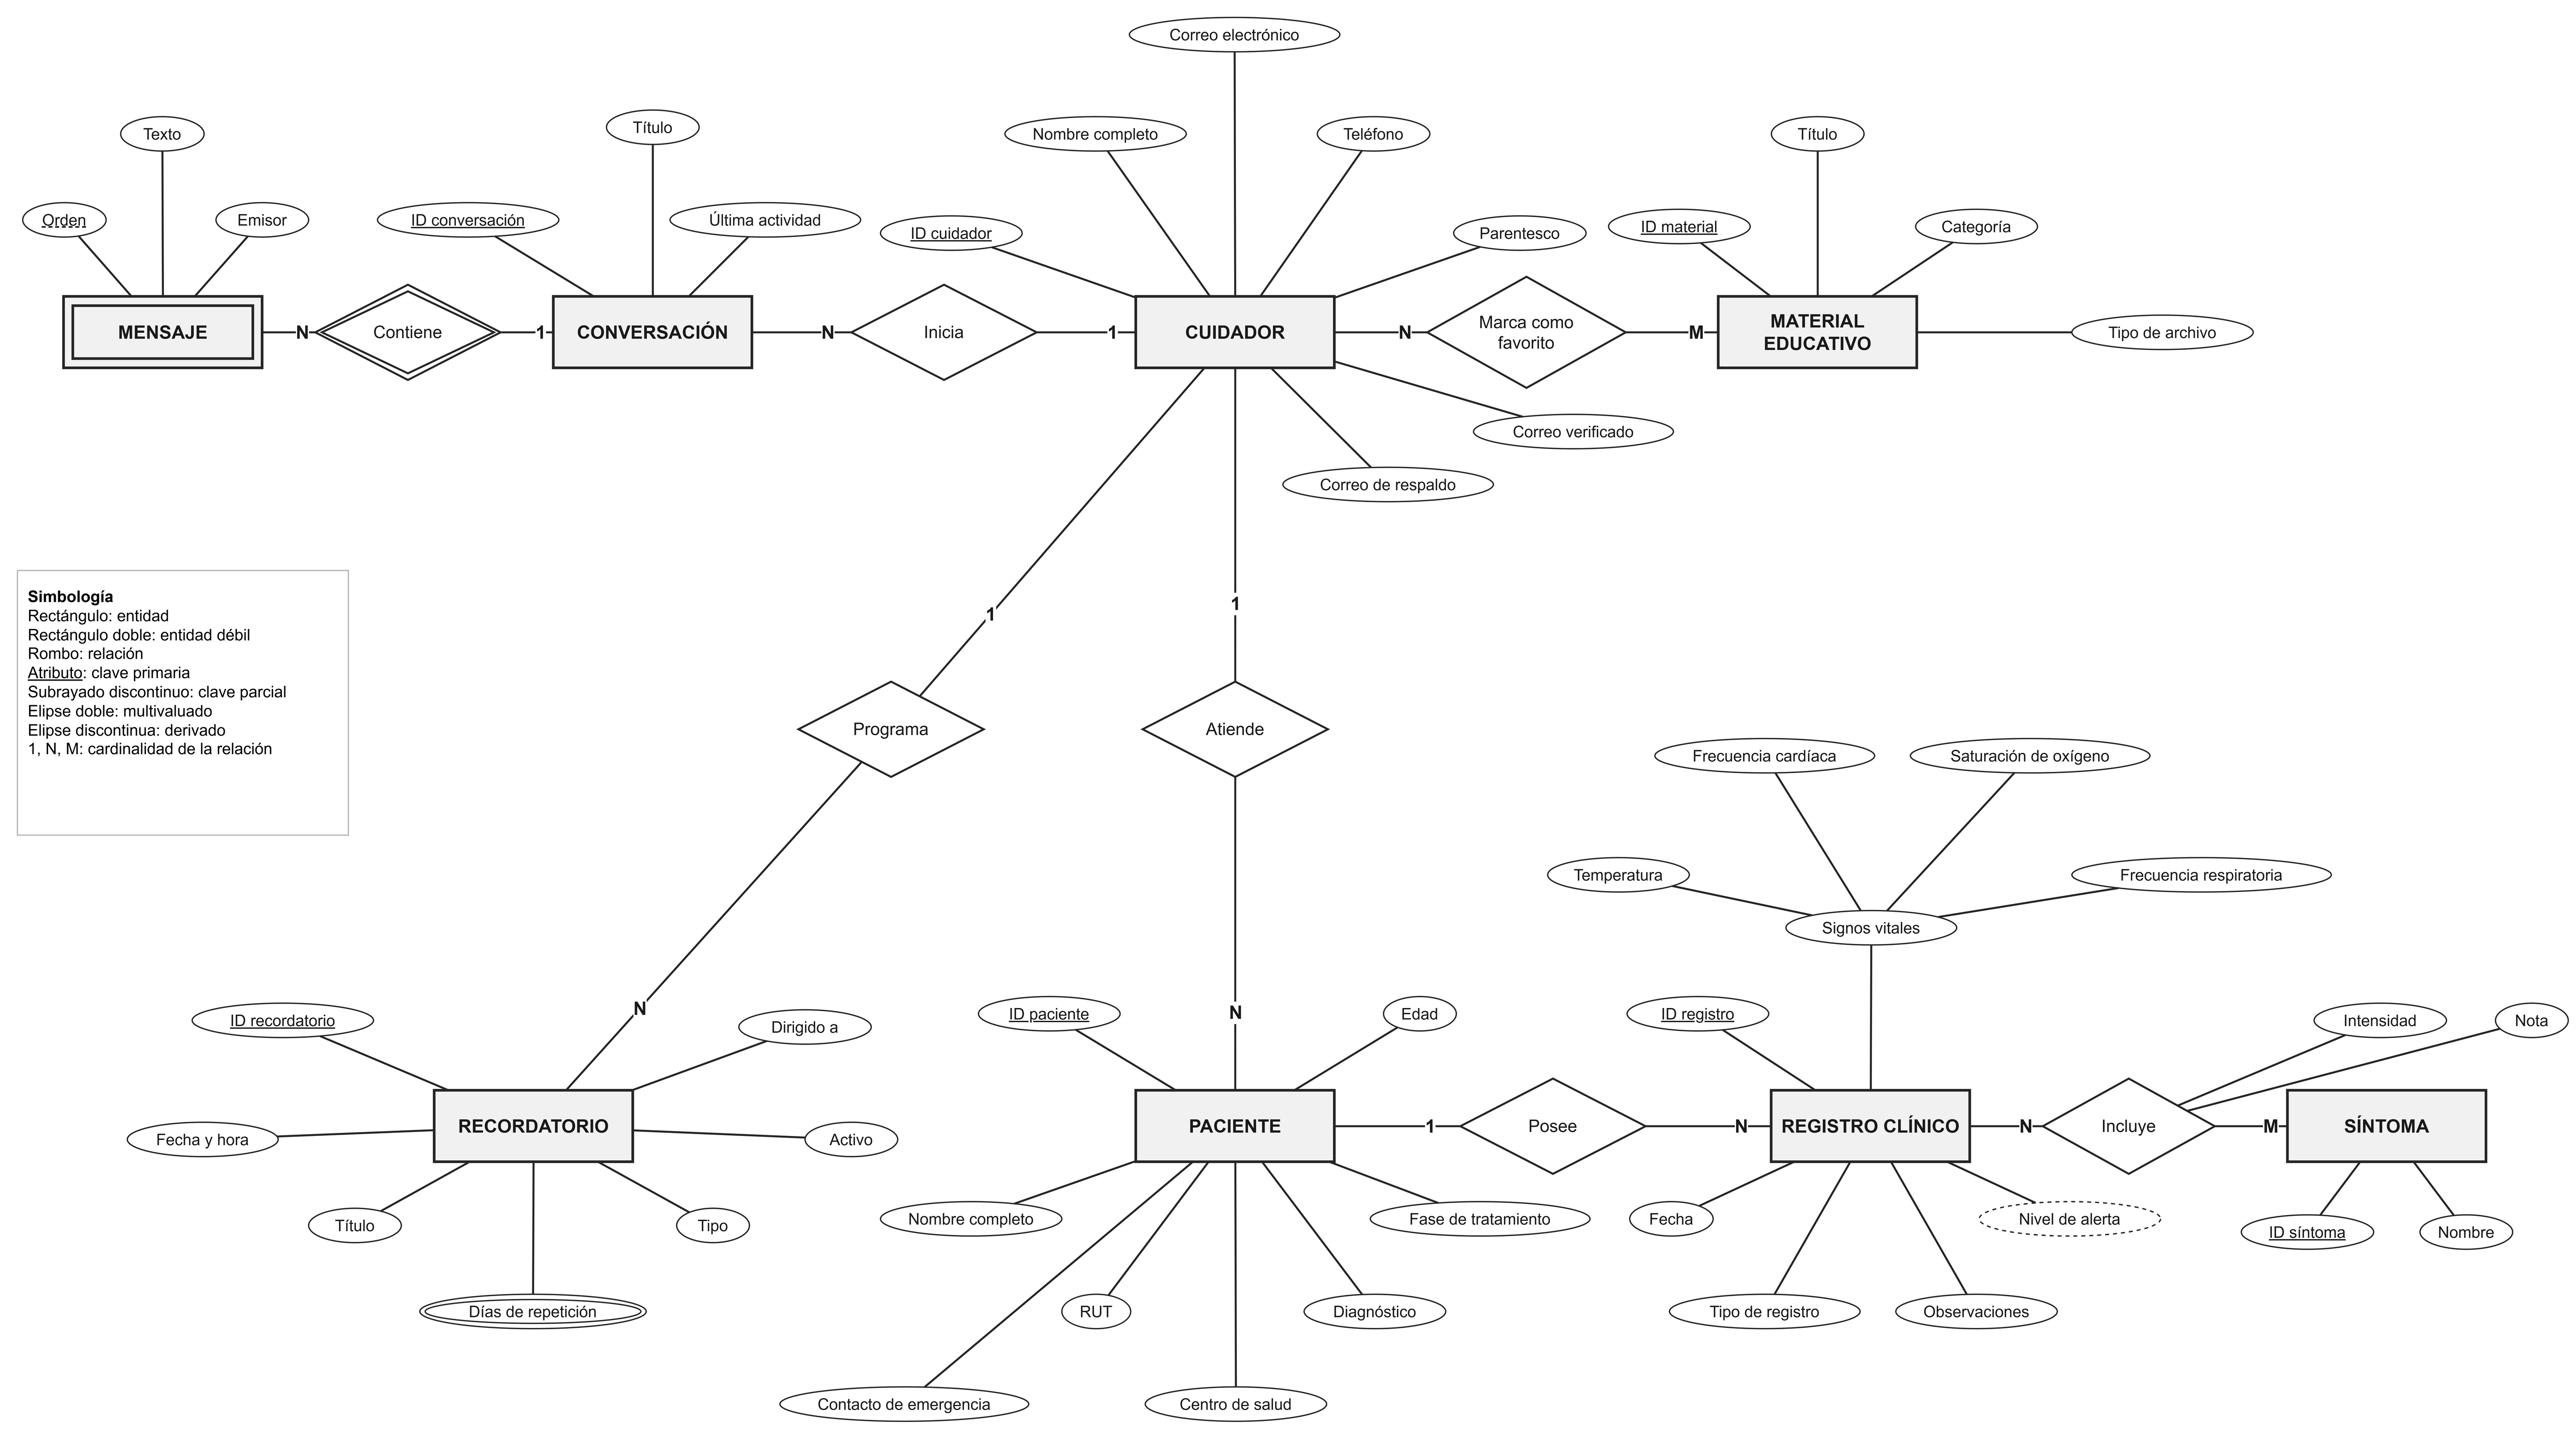
\includegraphics[width=\linewidth, height=0.93\textheight, keepaspectratio]{figures/mer/mer.png}
    \caption{Modelo entidad-relación de OnCuidar.}
    \label{fig:modelo-datos}
\end{figure}
\end{landscape}
\restoregeometry

Al pasar al modelo físico, cada entidad del modelo conceptual se transforma en
una tabla relacional de PostgreSQL (Tabla~\ref{tab:paso-fisico}). El cuidador
corresponde a la tabla usuarios y su identificador es la clave primaria. Las
tablas pacientes, conversaciones y favoritos llevan una clave foránea
a usuarios, y registros\_clinicos y recordatorios dependen del
paciente mediante una clave foránea compuesta (usuario y paciente), de modo que
todos los datos de una cuenta se eliminan en cascada al borrarla. La relación
N:M entre el cuidador y el material educativo se resuelve con la tabla puente
favoritos, de clave primaria compuesta, mientras que el catálogo
material\_educativo es compartido y no pertenece a ningún usuario.

El servidor no puede leer los datos clínicos, porque el dispositivo los cifra
antes de enviarlos. Por eso cada tabla combina columnas en claro, que el
servidor necesita para ordenar, filtrar y relacionar (fechas, nivel de alerta,
tipo de registro, estado activo o archivado), con una columna cifrados de
tipo jsonb que contiene el resto de los atributos como texto cifrado. El
modelo conceptual conserva las entidades Síntoma y Mensaje porque expresan el
dominio del problema, pero no se convierten en tablas propias: la intensidad y
la nota de cada síntoma viven dentro del contenido cifrado del registro clínico,
el catálogo ESAS se incluye en la propia aplicación, y los mensajes forman parte
del contenido cifrado de su conversación, ordenados por su posición. Del mismo
modo, el atributo compuesto de signos vitales y los días de repetición de un
recordatorio se almacenan dentro del jsonb cifrado. Además, el diseño físico
incorpora cuatro tablas de apoyo que no corresponden a entidades del dominio:
claves\_datos, tokens\_restablecer, tokens\_correo y
esperas\_recuperacion, que resuelven la seguridad de la cuenta. El
Anexo~E detalla todas las columnas.

\begin{table}[H]
\centering
\small
\tablazebra
\caption{Transformación del modelo conceptual a tablas relacionales.}
\label{tab:paso-fisico}
\begin{tabularx}{\textwidth}{P{0.90}P{1.00}P{1.10}}
\toprule
\filaencabezado \encab{Elemento conceptual} & \encab{Tabla o estructura física} & \encab{Clave y relación} \\
\midrule
Cuidador & usuarios & Clave primaria uuid; correo único. \\
Paciente & pacientes & Clave primaria (usuario, paciente); clave foránea a usuarios. \\
Registro clínico & registros\_clinicos & Clave primaria (usuario, paciente, registro); clave foránea compuesta a pacientes. \\
Recordatorio & recordatorios & Misma clave compuesta; el paciente al que se dirige es la clave foránea. \\
Conversación y Mensaje & conversaciones & Clave primaria (usuario, conversación); los mensajes van en el jsonb cifrado. \\
Material educativo & material\_educativo & Clave primaria de texto; catálogo compartido. \\
Marca como favorito (N:M) & favoritos & Tabla puente con clave primaria (usuario, material). \\
Síntoma e Incluye (N:M) & Contenido cifrado del registro & Catálogo en la aplicación; sin tabla propia. \\
\bottomrule
\end{tabularx}
\end{table}


\addtocontents{toc}{\protect\setcounter{tocdepth}{1}}
\chapter[Diseño]{Diseño}

\section[Diseño Físico de la Base de Datos]{Diseño físico de la base de datos}

La base de datos se implementa en PostgreSQL 15, un motor relacional que se
ejecuta en un contenedor y solo es accesible desde la API a través de una red
interna. La estructura sigue la transformación del modelo conceptual descrita en
el capítulo anterior: cada cuidador es la raíz de sus datos y las tablas que
dependen de él llevan una clave foránea con eliminación en cascada
(\texttt{ON DELETE CASCADE}), de modo que al borrar la cuenta se eliminan sus
pacientes, registros, recordatorios, conversaciones, favoritos y claves. El
Listado~\ref{lst:esquema-sql} resume el esquema y el Anexo~E describe cada
columna. Las columnas jsonb llamadas cifrados contienen únicamente texto cifrado
con AES-256-GCM en el teléfono del cuidador, y el servidor no dispone de la clave
para descifrarlas.

\begin{lstlisting}[language={},basicstyle=\ttfamily\fontsize{7.2pt}{8.6pt}\selectfont,columns=fullflexible,breaklines=true,caption={Esquema relacional resumido de OnCuidar (PostgreSQL 15).},label={lst:esquema-sql}]
CREATE TABLE usuarios (            -- cuidador
  id uuid PRIMARY KEY DEFAULT gen_random_uuid(),
  correo text UNIQUE NOT NULL,
  contrasena_hash text,            -- bcrypt
  correo_verificado boolean DEFAULT false,
  correo_respaldo_hash text,       -- solo HMAC del correo de respaldo
  cifrados jsonb DEFAULT '{}',     -- nombre, telefono, parentesco (cifrados)
  creado_en timestamptz DEFAULT now() );   -- y columnas de correos pendientes

CREATE TABLE pacientes (
  usuario_id uuid REFERENCES usuarios(id) ON DELETE CASCADE,
  id text,
  notificaciones_activas boolean, maximo_registros_dia int, archivado boolean,
  cifrados jsonb,                  -- nombre, RUT, edad, diagnostico, centro, contacto
  PRIMARY KEY (usuario_id, id) );

CREATE TABLE registros_clinicos (
  usuario_id uuid, paciente_id text, id text,
  fecha timestamptz, tipo_registro text, nivel_alerta text,   -- en claro
  cifrados jsonb,                  -- signos vitales, sintomas, observaciones
  PRIMARY KEY (usuario_id, paciente_id, id),
  FOREIGN KEY (usuario_id, paciente_id) REFERENCES pacientes
    ON DELETE CASCADE );           -- indices por (usuario, paciente, fecha/creado_en)

CREATE TABLE recordatorios (
  usuario_id uuid, paciente_id text, id text, activo boolean,
  cifrados jsonb,                  -- titulo, descripcion, programacion
  PRIMARY KEY (usuario_id, paciente_id, id),
  FOREIGN KEY (usuario_id, paciente_id) REFERENCES pacientes
    ON DELETE CASCADE );

CREATE TABLE conversaciones (
  usuario_id uuid REFERENCES usuarios(id) ON DELETE CASCADE,
  id text, ultima_actividad timestamptz,
  cifrados jsonb,                  -- titulo y mensajes
  PRIMARY KEY (usuario_id, id) );

CREATE TABLE material_educativo ( -- catalogo compartido, de solo lectura
  id text PRIMARY KEY, titulo text, categoria text, tema text, cuerpo text,
  url_imagen text, url_archivo text, url_miniatura text,
  tipo_archivo text, tamano_bytes bigint );

CREATE TABLE favoritos (          -- tabla puente N:M
  usuario_id uuid REFERENCES usuarios(id) ON DELETE CASCADE,
  material_id text,
  PRIMARY KEY (usuario_id, material_id) );

CREATE TABLE claves_datos (       -- clave de datos sellada con la clave maestra
  usuario_id uuid PRIMARY KEY REFERENCES usuarios(id) ON DELETE CASCADE,
  clave_sellada text NOT NULL );

CREATE TABLE tokens_restablecer ( -- enlaces de un solo uso (1 h), solo hash
  token_hash text PRIMARY KEY, usuario_id uuid REFERENCES usuarios(id)
    ON DELETE CASCADE, expira_en timestamptz, usado boolean );
-- tokens_correo (verificacion y cambio de correos) y esperas_recuperacion
-- (limite de reenvios) siguen el mismo patron.
\end{lstlisting}

El motor admite funciones y disparadores, pero el diseño concentra las reglas de
integridad en las claves y en la API, que aplican las siguientes restricciones.

\begin{itemize}
    \item \emph{Integridad referencial}: las claves foráneas, simples o
    compuestas, impiden crear un registro clínico o un recordatorio sin su
    paciente, y la eliminación en cascada evita datos huérfanos.
    \item \emph{Índices}: los registros clínicos y los recordatorios tienen un
    índice por usuario, paciente y fecha de creación, y las conversaciones por
    usuario y última actividad, que son los órdenes con que la aplicación
    lista los datos.
    \item \emph{Autorización por usuario}: cada petición lleva un token JWT y
    toda consulta se filtra por el usuario del token. Un recurso de otro
    usuario responde como inexistente.
    \item \emph{Datos sensibles cifrados}: la API rechaza con error 400 cualquier
    escritura que incluya un campo clínico en claro, y solo acepta en la columna
    cifrados claves que corresponden a texto cifrado.
    \item \emph{Contenido educativo}: la tabla material\_educativo es de solo
    lectura para la aplicación. La API la carga al iniciar si está vacía.
    \item \emph{Clave de datos}: la ruta \texttt{POST /clave-datos} crea la clave
    de cifrado del usuario la primera vez y la sella con AES-256-GCM usando una
    clave maestra definida en el entorno del servidor. La tabla claves\_datos
    solo guarda la clave sellada, y el cliente nunca accede a ella directamente.
    \item \emph{Credenciales y enlaces}: las contraseñas se guardan con bcrypt y
    los enlaces de correo, que son de un solo uso y vencen en una hora, solo
    registran el hash de su token. El correo de respaldo se conserva únicamente
    como HMAC.
\end{itemize}

\section[Diseño de Arquitectura Funcional]{Diseño de arquitectura funcional}

La Figura~\ref{fig:arquitectura} descompone el sistema en siete módulos
funcionales. Sus funciones corresponden a los casos de uso del capítulo
anterior.

\begin{figure}[H]
    \centering
    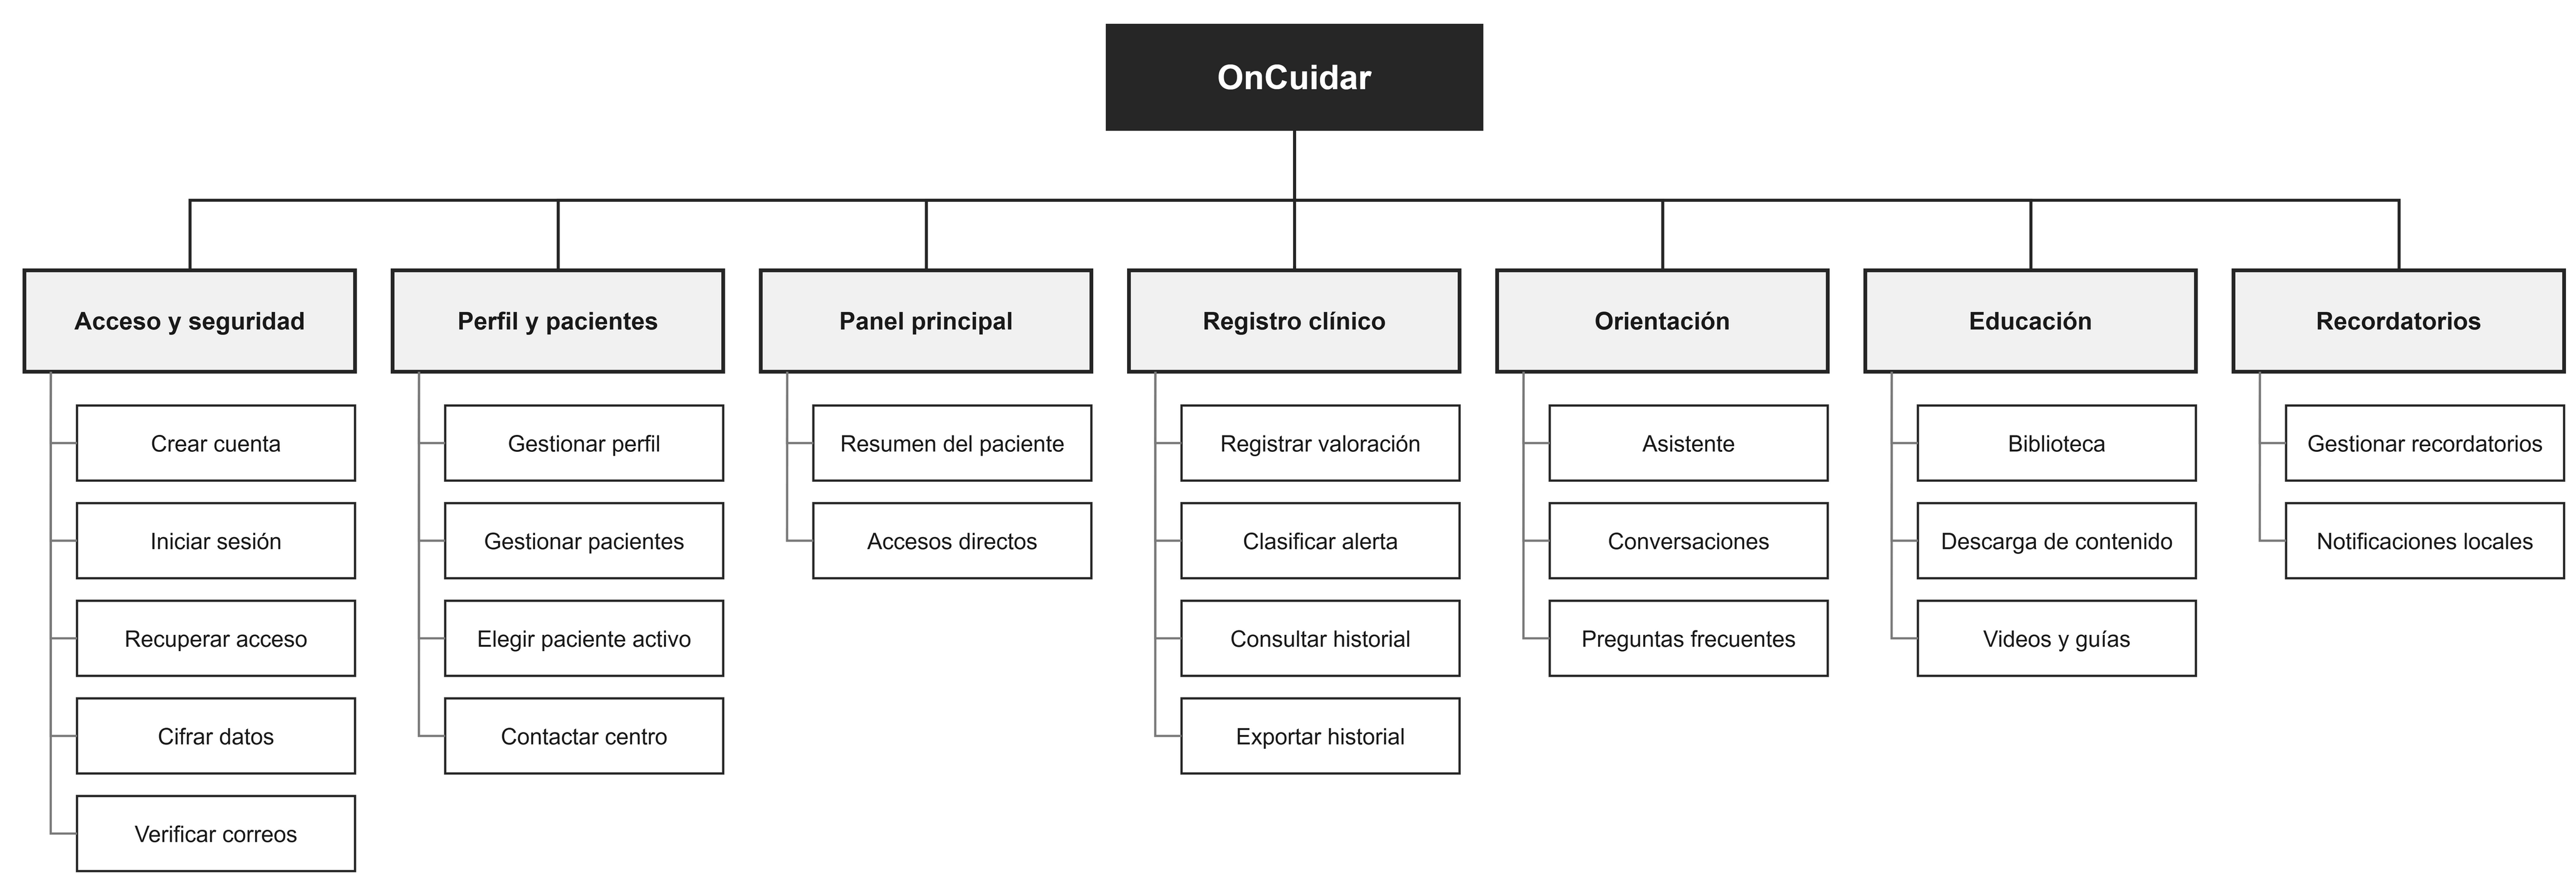
\includegraphics[width=\textwidth]{figures/diseno/arquitectura.png}
    \caption{Árbol de descomposición funcional de OnCuidar.}
    \label{fig:arquitectura}
\end{figure}

Internamente, el código se organiza por funcionalidad y, dentro de cada una,
en tres capas, siguiendo la guía de arquitectura de aplicaciones de Flutter. Cada
funcionalidad (autenticación, pacientes, registro clínico, historial, panel
principal, chat, preguntas frecuentes, recordatorios, biblioteca y perfil) tiene
una carpeta de dominio, con los modelos y las reglas puras, como el motor de
reglas clínicas; una de datos, con el repositorio que guarda y lee en la API del
servidor cifrando y descifrando los campos sensibles; y una de presentación, con las
pantallas, sus widgets y un controlador que reúne la lógica de cada pantalla. El
estado se expone a las pantallas con Riverpod y se actualiza mediante consultas
periódicas a la API, en lugar de suscripciones en tiempo real.

Los repositorios comparten una base de datos segura común, que concentra el
cifrado, la cola de escrituras sin conexión y la identidad del cuidador, pero no
dependen entre sí. Cuando una acción involucra a más de un área, la coordina un
caso de uso: por ejemplo, archivar o eliminar un paciente también cancela los
avisos de sus recordatorios. Los servicios transversales (cifrado,
conectividad, notificaciones y sincronización) forman un núcleo común, y los
componentes visuales reutilizados por varias pantallas, una carpeta compartida.
Esta separación permite probar cada capa de forma aislada y modificar una
pantalla sin tocar la lógica de datos.

Al iniciar sesión, una compuerta de datos restaura la clave de cifrado del
usuario o la solicita al servidor antes de mostrar cualquier información del
paciente. Luego se descarga en segundo plano el contenido educativo para dejarlo
disponible sin conexión.

\section[Diseño de Arquitectura Física y Despliegue]{Diseño de arquitectura física y despliegue}

La Figura~\ref{fig:despliegue} muestra la arquitectura física. El cuidador
usa la aplicación Flutter en un teléfono Android, que cifra los datos sensibles
con AES-GCM antes de enviarlos y guarda en un almacenamiento seguro el token de
sesión y la clave de datos. La aplicación se comunica con la API mediante
HTTP y JSON, con el token JWT en cada petición; si no hay conexión, la cola de
escrituras conserva las operaciones y las envía al recuperar la red.

\begin{figure}[H]
    \centering
    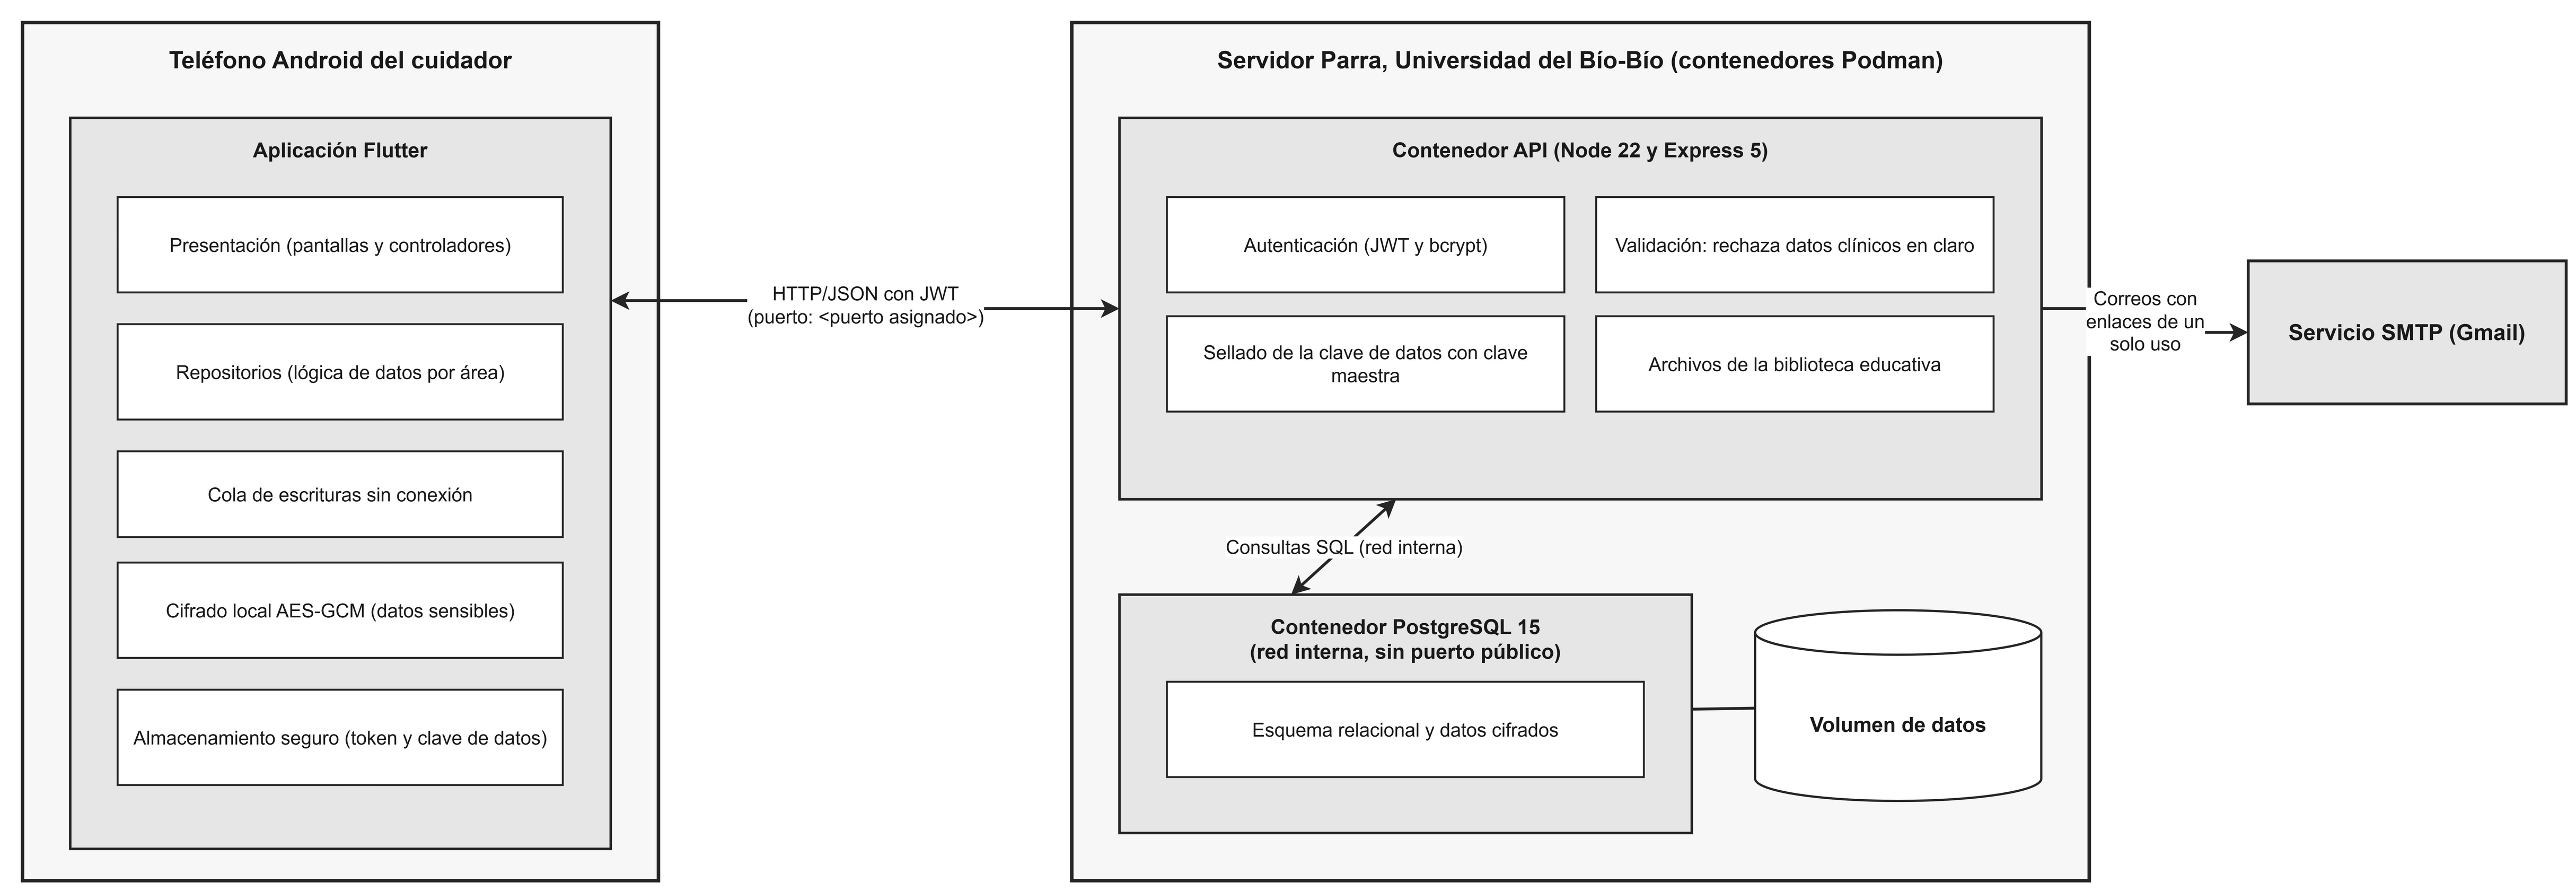
\includegraphics[width=\textwidth]{figures/diseno/despliegue.png}
    \caption{Arquitectura física y despliegue de OnCuidar.}
    \label{fig:despliegue}
\end{figure}

El servidor ejecuta dos contenedores definidos en Docker Compose y destinados a
Podman en el servidor Parra de la Universidad del Bío-Bío. El contenedor de la API
(Node 22 y Express 5) es el único que publica un puerto y también sirve los
archivos de la biblioteca educativa. El contenedor de PostgreSQL permanece en la
red interna, sin puerto público, y guarda sus datos en un volumen persistente. Para
enviar los correos de verificación y recuperación, la API utiliza un servicio
SMTP externo (Gmail). El sistema funciona en un entorno local; su despliegue en
el servidor de la universidad queda pendiente de la activación de la cuenta y de
la entrega de los puertos definitivos. La Tabla~\ref{tab:puertos} resume los
servicios.

\begin{table}[H]
\centering
\small
\tablazebra
\caption{Servicios del despliegue y su exposición.}
\label{tab:puertos}
\begin{tabularx}{\textwidth}{P{0.80}P{0.90}P{0.70}P{0.60}}
\toprule
\filaencabezado \encab{Servicio} & \encab{Función} & \encab{Puerto} & \encab{Acceso} \\
\midrule
API (Node y Express) & Autenticación, validación y acceso a datos & \textless puerto asignado\textgreater{} (3000 en el contenedor) & Público, con JWT \\
PostgreSQL 15 & Almacenamiento relacional de los datos cifrados & 5432 solo en la red interna & Solo la API \\
Servicio SMTP (Gmail) & Entrega de correos con enlaces de un solo uso & Definido por el proveedor & Salida desde la API \\
\bottomrule
\end{tabularx}
\end{table}

\section[Diseño de Interfaz y Navegación]{Diseño de interfaz y navegación}

\subsection*{Estándar de pantalla}

Todas las pantallas siguen el mismo esquema.

\begin{itemize}
    \item \emph{Encabezado}: cabecera con degradado dorado, título de la
    pantalla y, en el panel principal, saludo y nombre del paciente activo.
    \item \emph{Logo}: la marca OnCuidar aparece en la carga inicial, la
    bienvenida y el pie del perfil.
    \item \emph{Ingreso de datos}: campos con etiqueta visible, validación en
    línea y mensajes de error bajo el campo afectado.
    \item \emph{Botones de opción general}: acción principal destacada en
    dorado (guardar, crear, continuar) y acción secundaria con contorno
    (cancelar, volver).
    \item \emph{Botones específicos}: acciones propias de cada pantalla, como
    exportar en el historial o marcar como favorito en la biblioteca.
    \item \emph{Menú}: barra inferior permanente con Inicio, Chat, Registro,
    Aprende y Perfil.
    \item \emph{Estados de alerta}: verde, amarillo y rojo, siempre acompañados
    de un ícono y un texto.
\end{itemize}

\subsection*{Mapa de navegación}

La Figura~\ref{fig:navegacion} muestra las rutas de la aplicación. Si existe una
sesión activa, la carga inicial lleva directamente al panel principal. En caso
contrario, pasa por la bienvenida, desde donde el cuidador inicia sesión o crea
su cuenta. Una vez dentro, la barra inferior da acceso a los cinco módulos
principales y el panel principal ofrece accesos directos al historial y a los
recordatorios.

\begin{figure}[H]
    \centering
    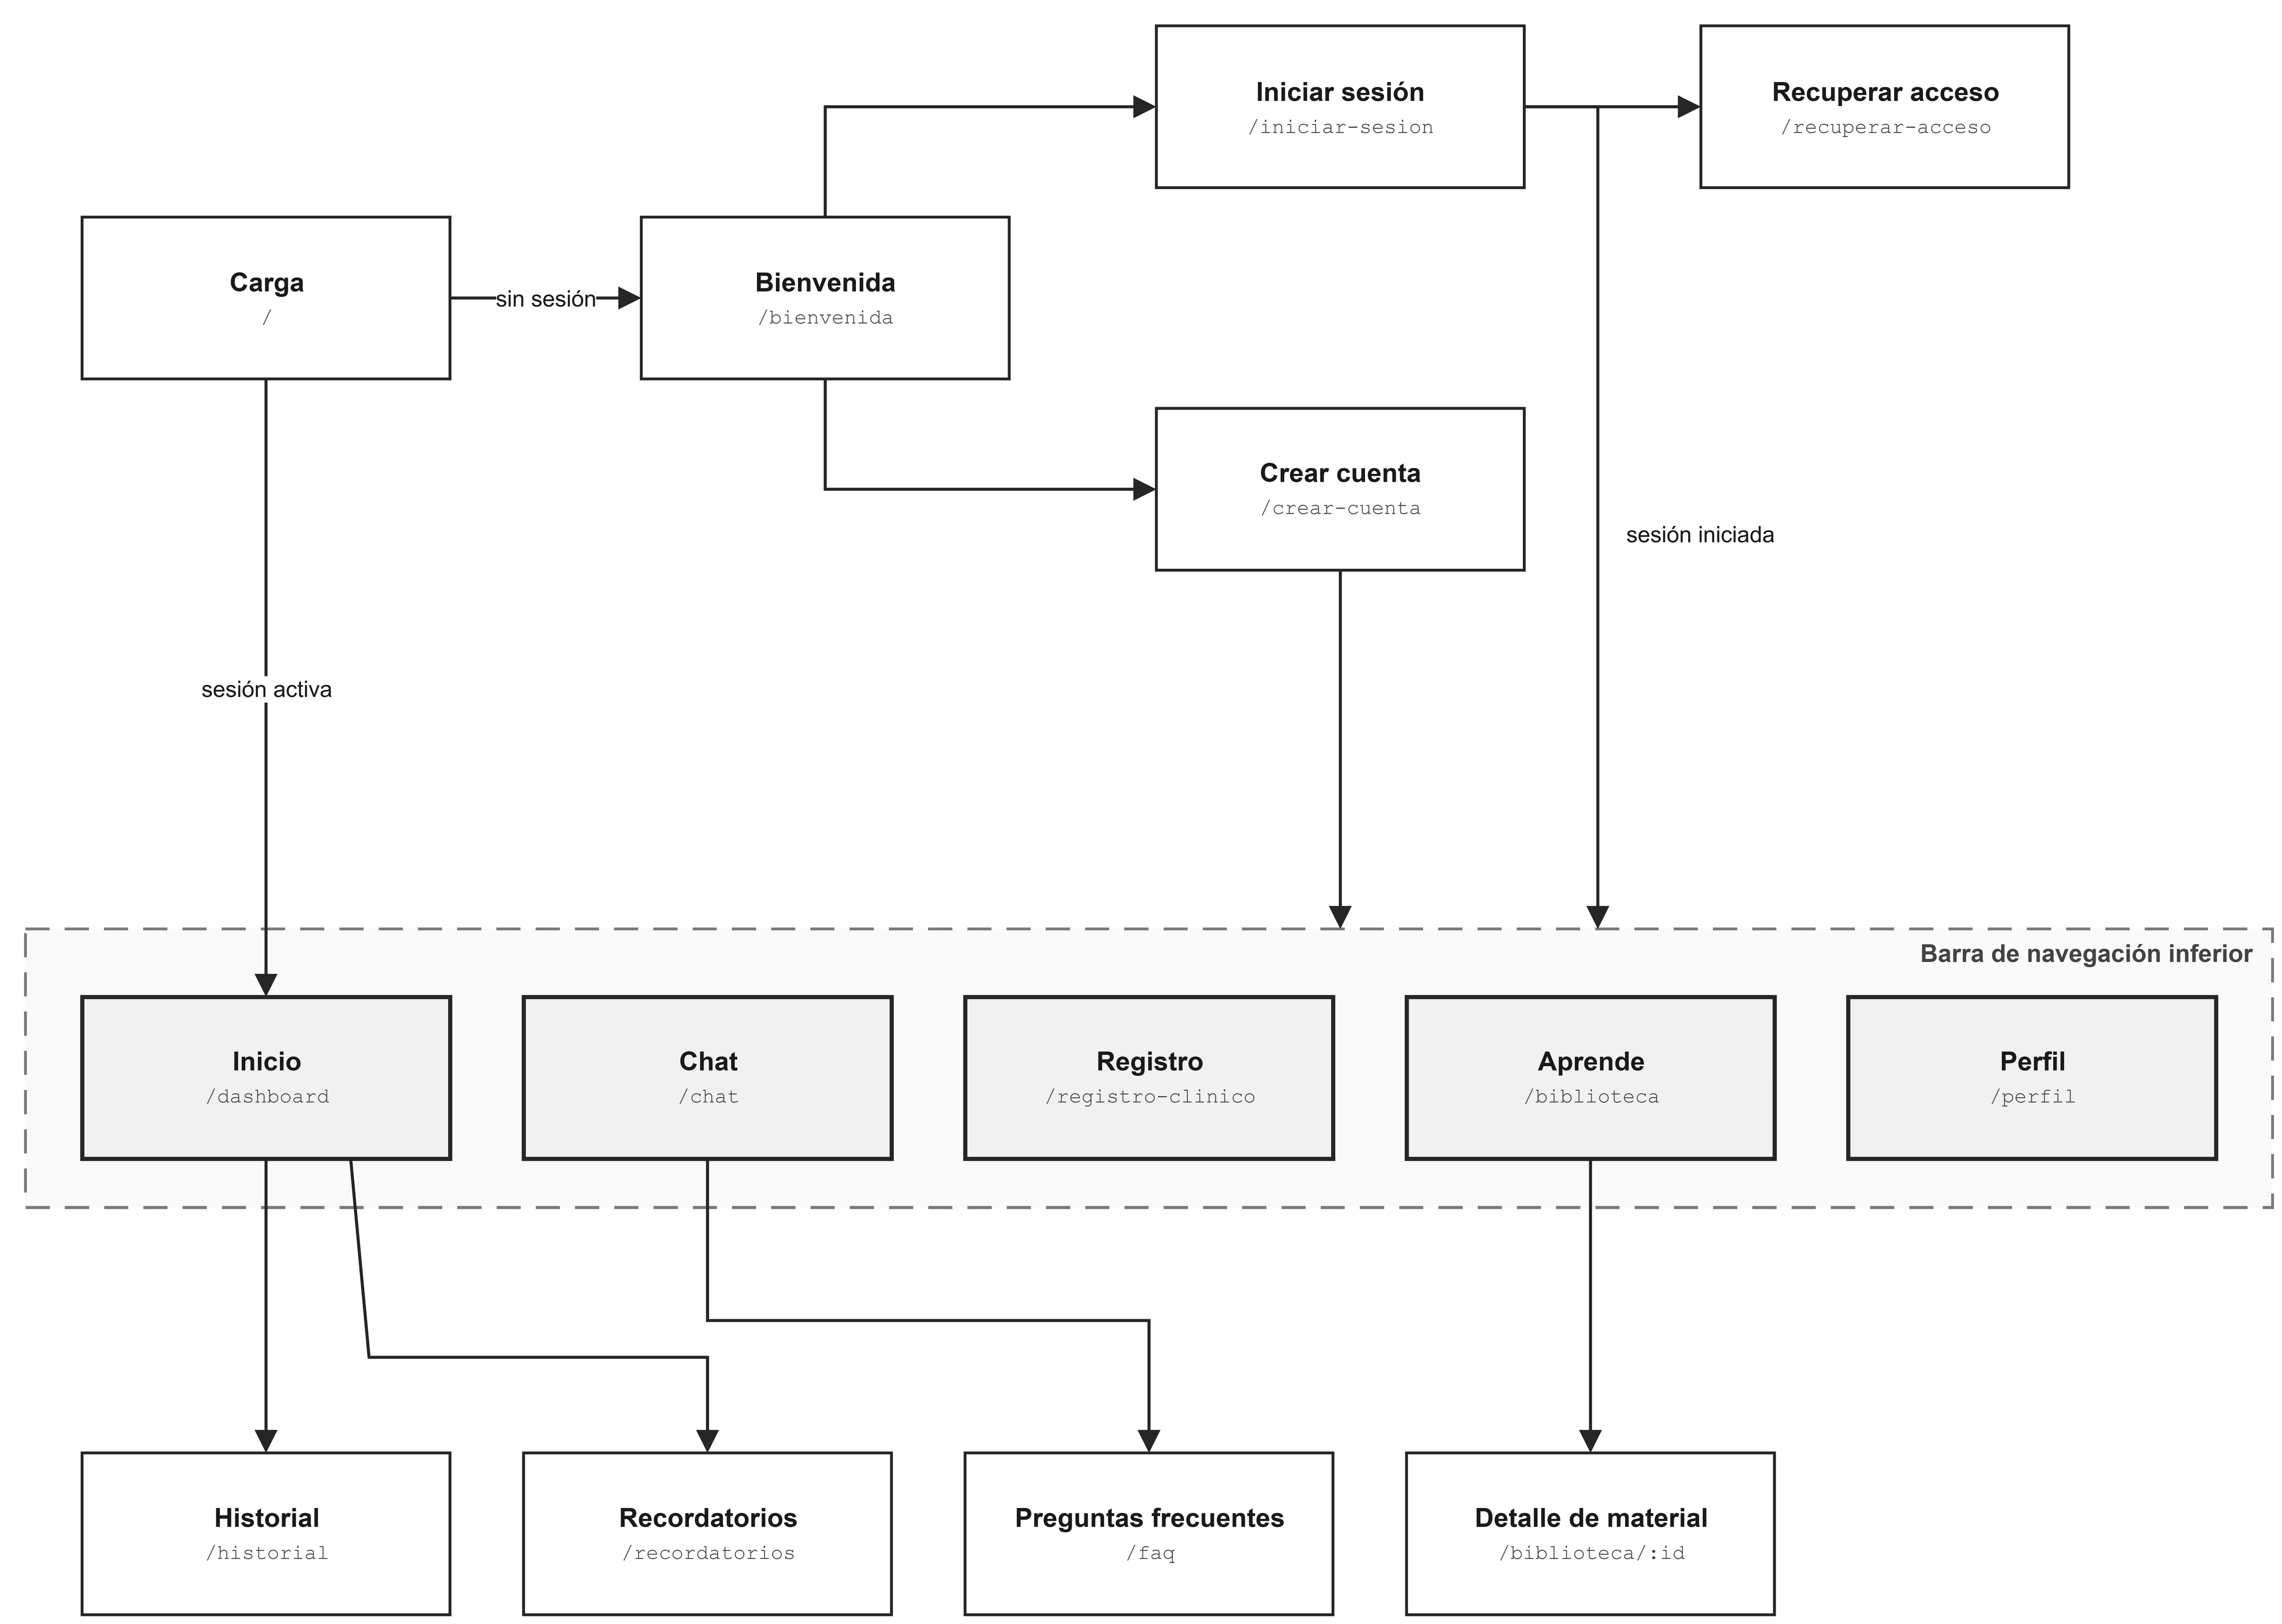
\includegraphics[width=0.95\textwidth]{figures/diseno/navegacion.png}
    \caption{Mapa de navegación de OnCuidar.}
    \label{fig:navegacion}
\end{figure}

\subsection*{Prototipos de interfaz}

Los prototipos se diseñaron en Figma y se revisaron con la contraparte antes de
construir cada módulo. La paleta cálida, inspirada en el lazo dorado del cáncer
infantil, busca transmitir cercanía y reducir la fatiga visual. Las figuras
siguientes presentan el acceso, el seguimiento, el apoyo educativo y la gestión.

\begin{figure}[H]
    \centering
    \begin{subfigure}[b]{0.30\textwidth}
        \centering
        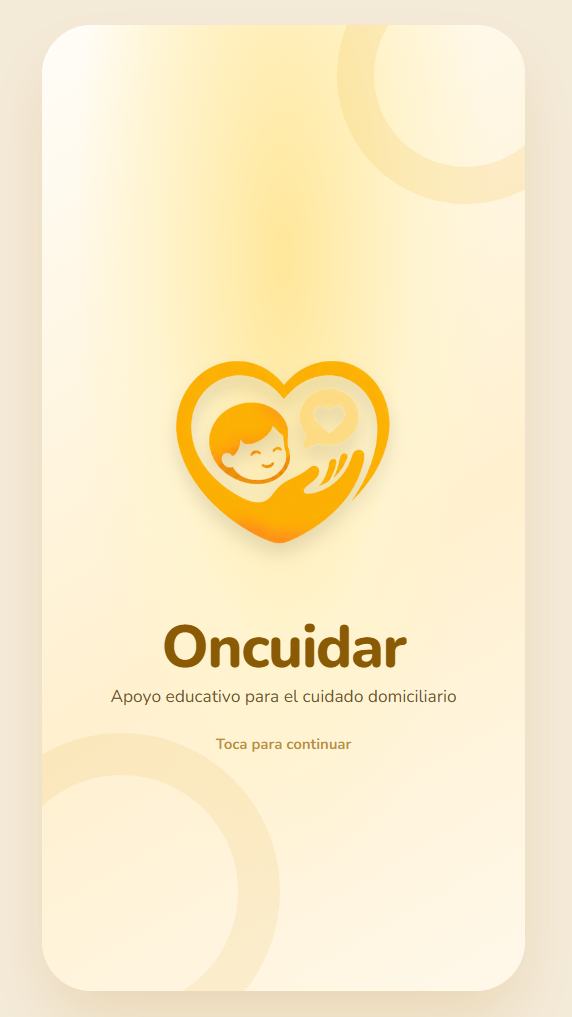
\includegraphics[width=\linewidth]{figures/mockups/01_splash.png}
        \caption{Pantalla de inicio}
        \label{fig:mockup-splash}
    \end{subfigure}
    \hfill
    \begin{subfigure}[b]{0.30\textwidth}
        \centering
        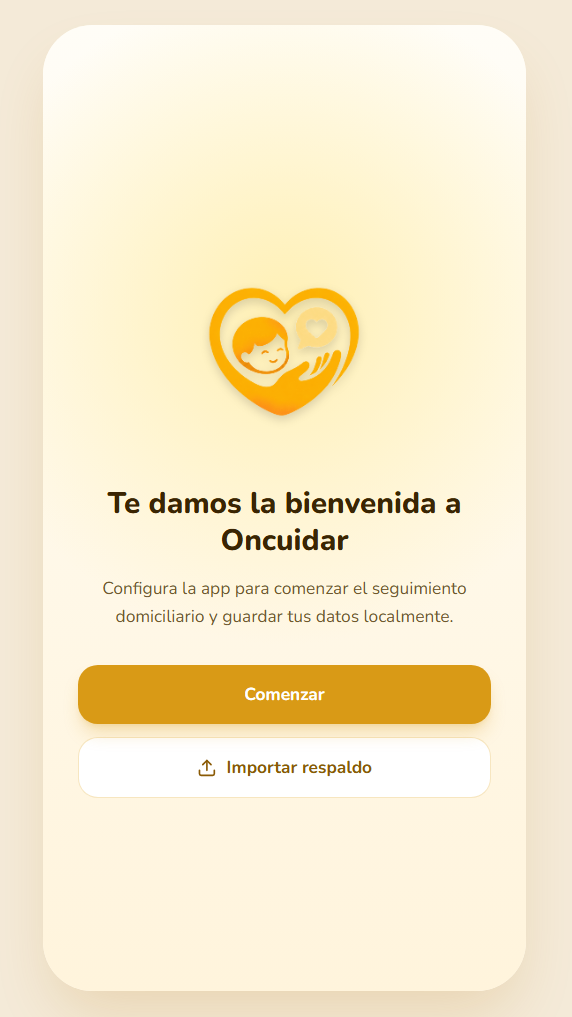
\includegraphics[width=\linewidth]{figures/mockups/02_bienvenida.png}
        \caption{Bienvenida}
        \label{fig:mockup-bienvenida}
    \end{subfigure}
    \hfill
    \begin{subfigure}[b]{0.30\textwidth}
        \centering
        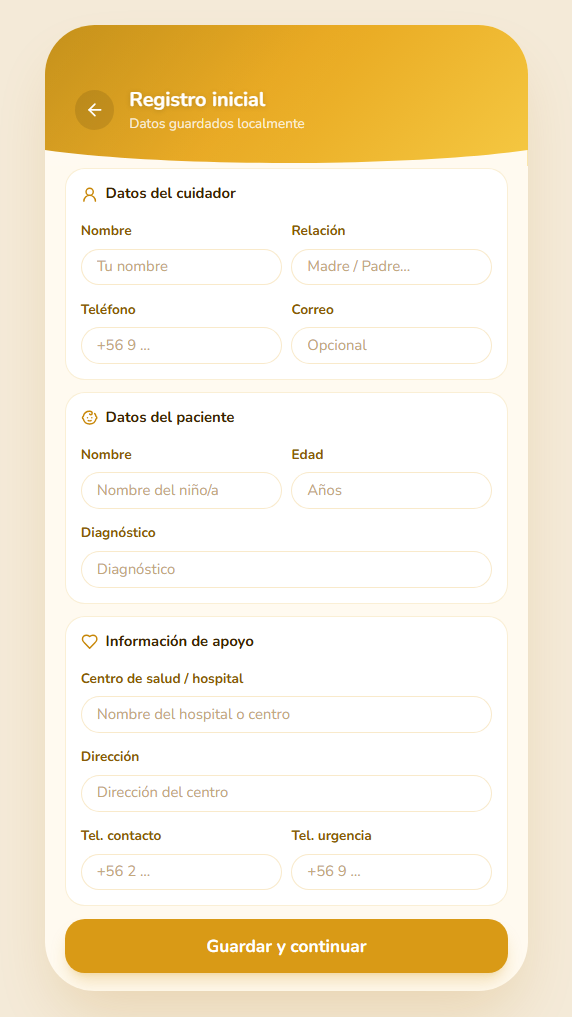
\includegraphics[width=\linewidth]{figures/mockups/03_registro_inicial.png}
        \caption{Registro inicial}
        \label{fig:mockup-registro-inicial}
    \end{subfigure}
    \caption{Flujo de \textit{onboarding}: acceso al sistema y configuración del perfil.}
    \label{fig:mockups-flujo-inicial}
\end{figure}

\begin{figure}[H]
    \centering
    \begin{subfigure}[b]{0.30\textwidth}
        \centering
        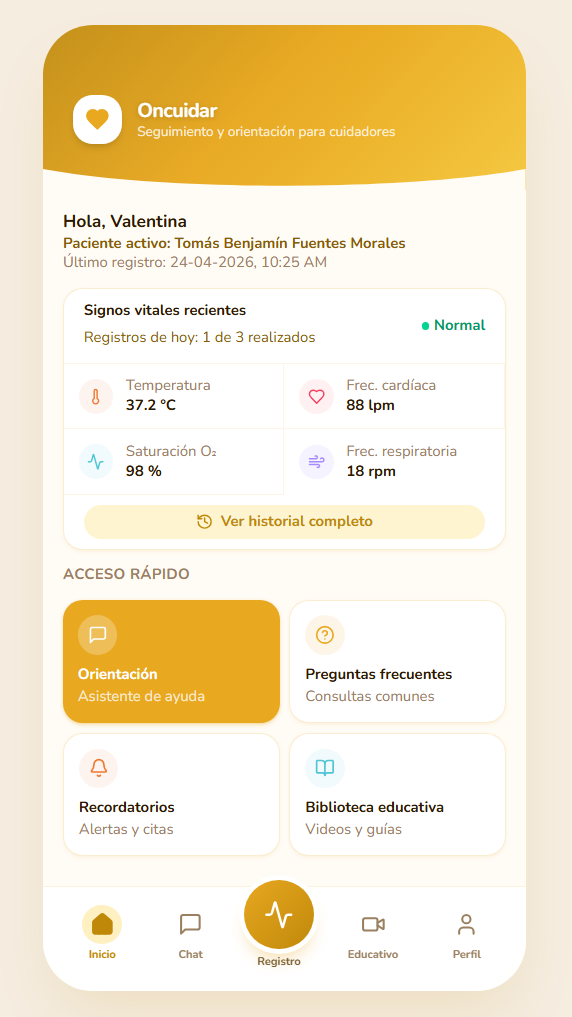
\includegraphics[width=\linewidth]{figures/mockups/04_inicio.png}
        \caption{Inicio (\textit{Dashboard})}
        \label{fig:mockup-inicio}
    \end{subfigure}
    \hfill
    \begin{subfigure}[b]{0.30\textwidth}
        \centering
        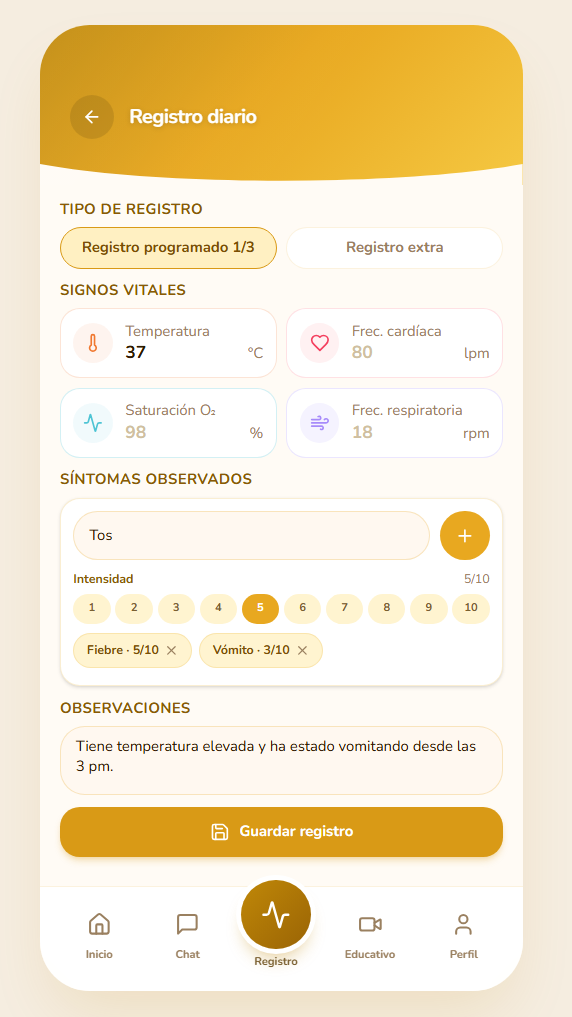
\includegraphics[width=\linewidth]{figures/mockups/05_registro_diario.png}
        \caption{Registro diario}
        \label{fig:mockup-registro-diario}
    \end{subfigure}
    \hfill
    \begin{subfigure}[b]{0.30\textwidth}
        \centering
        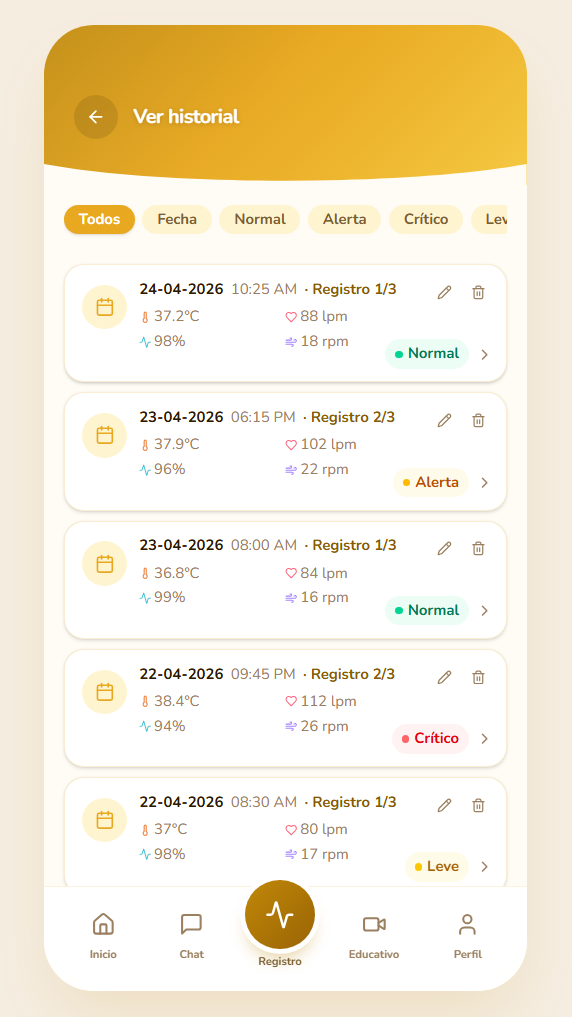
\includegraphics[width=\linewidth]{figures/mockups/06_historial.png}
        \caption{Historial clínico}
        \label{fig:mockup-historial}
    \end{subfigure}
    \caption{Módulo de bitácora: visualización del estado, ingreso de métricas y consulta cronológica.}
    \label{fig:mockups-seguimiento}
\end{figure}

\begin{figure}[H]
    \centering
    \begin{subfigure}[b]{0.30\textwidth}
        \centering
        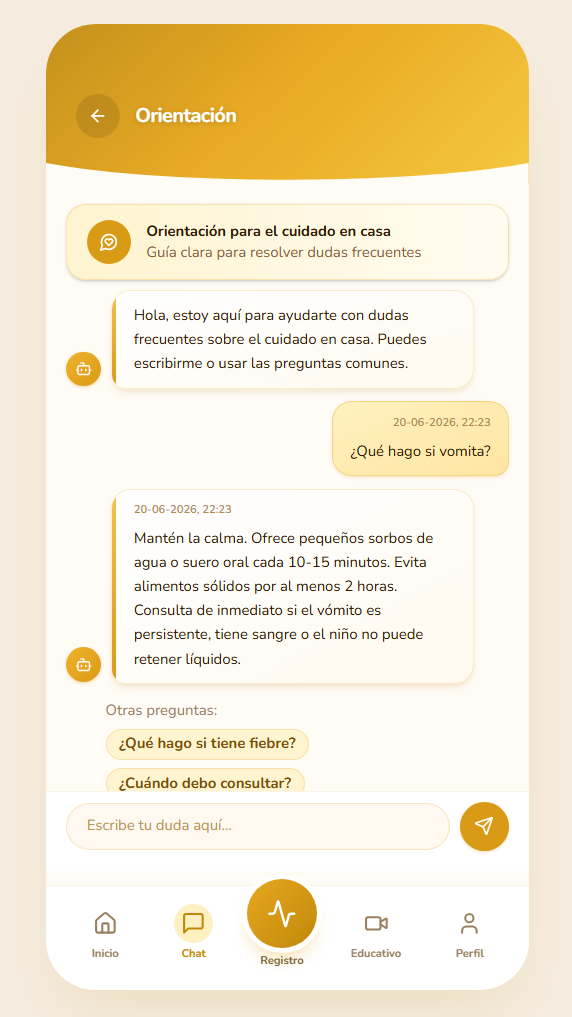
\includegraphics[width=\linewidth]{figures/mockups/07_orientacion.png}
        \caption{Orientación guiada}
        \label{fig:mockup-orientacion}
    \end{subfigure}
    \hfill
    \begin{subfigure}[b]{0.30\textwidth}
        \centering
        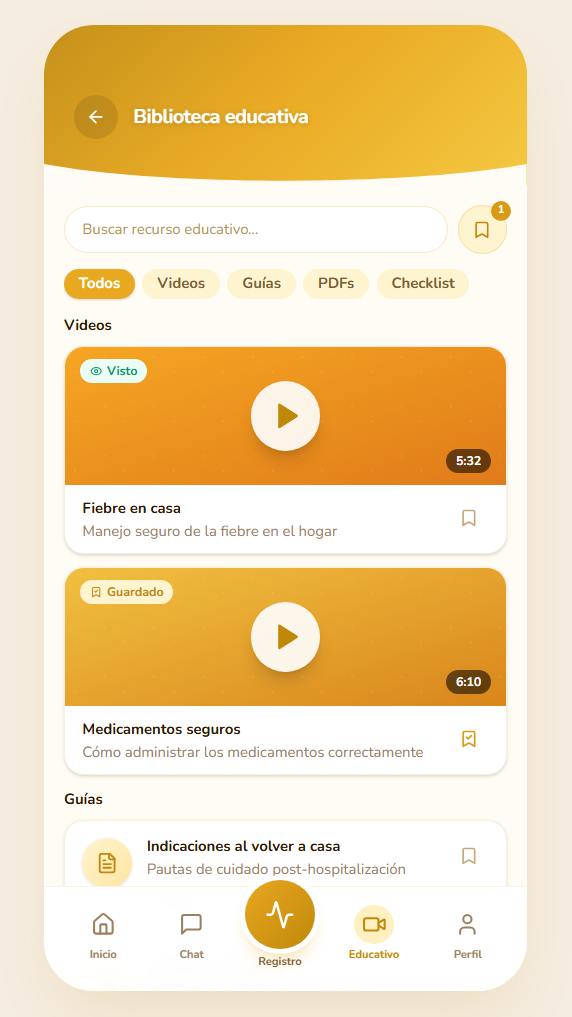
\includegraphics[width=\linewidth]{figures/mockups/08_biblioteca.png}
        \caption{Biblioteca de salud}
        \label{fig:mockup-biblioteca}
    \end{subfigure}
    \hfill
    \begin{subfigure}[b]{0.30\textwidth}
        \centering
        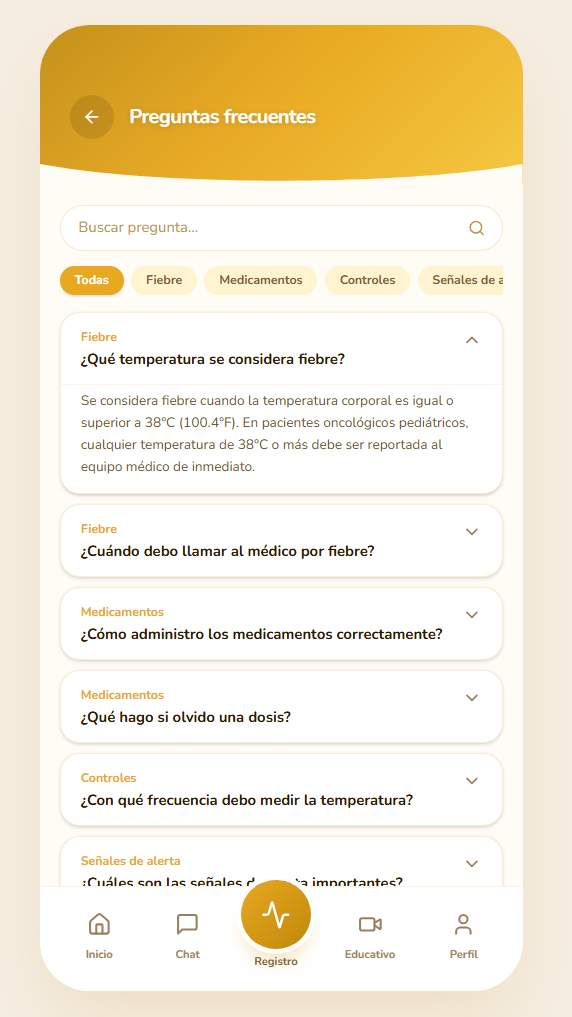
\includegraphics[width=\linewidth]{figures/mockups/09_preguntas_frecuentes.png}
        \caption{Preguntas frecuentes}
        \label{fig:mockup-preguntas}
    \end{subfigure}
    \caption{Módulo de apoyo: asistente de reglas, repositorio de lectura y resolución de dudas.}
    \label{fig:mockups-apoyo-educativo}
\end{figure}

\begin{figure}[H]
    \centering
    \begin{subfigure}[b]{0.30\textwidth}
        \centering
        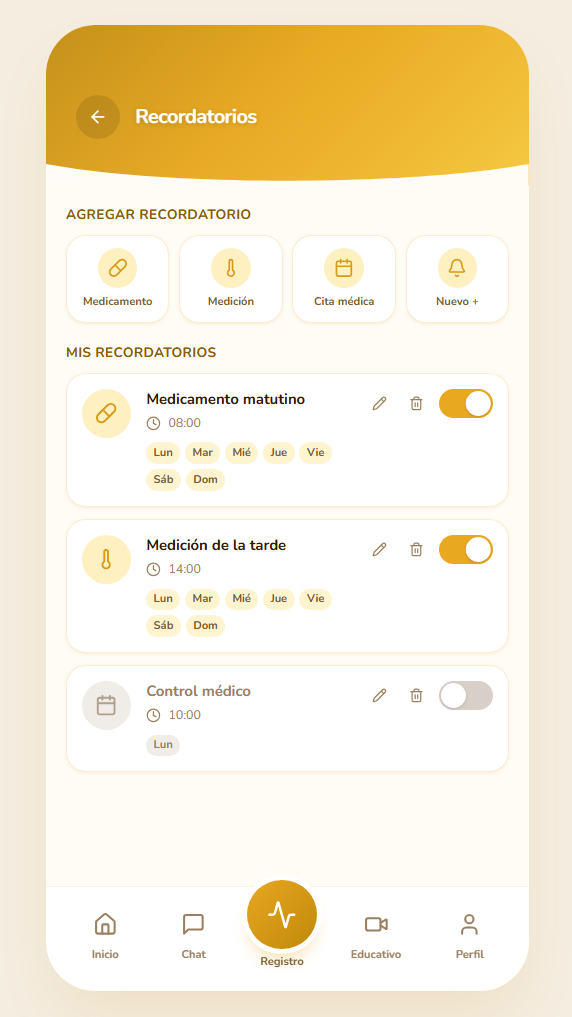
\includegraphics[width=\linewidth]{figures/mockups/10_recordatorios.png}
        \caption{Gestión de alarmas}
        \label{fig:mockup-recordatorios}
    \end{subfigure}
    \hfill
    \begin{subfigure}[b]{0.30\textwidth}
        \centering
        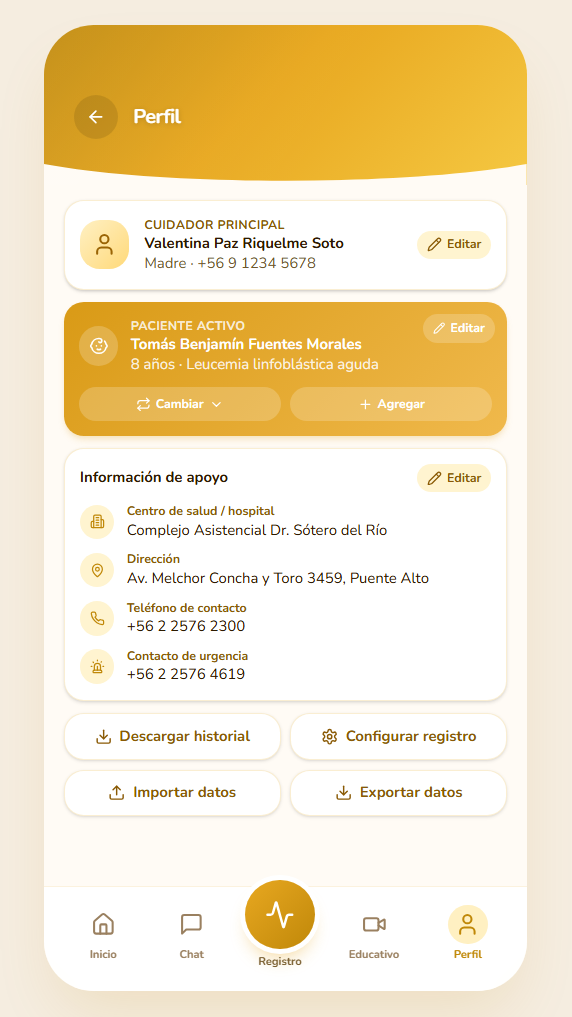
\includegraphics[width=\linewidth]{figures/mockups/11_perfil.png}
        \caption{Perfil y exportación de informes}
        \label{fig:mockup-perfil}
    \end{subfigure}
    \caption{Módulo de gestión: configuración de notificaciones y administración de datos.}
    \label{fig:mockups-gestion}
\end{figure}

\section[Especificación de Módulos]{Especificación de módulos}

La Tabla~\ref{tab:modulos} especifica los módulos de programa principales, con
sus parámetros de entrada y de salida.

\begingroup
\small
\tablazebra
\begin{xltabular}{\textwidth}{P{0.35}P{1.05}P{1.40}P{1.20}}
    \caption{Especificación de los módulos de programa.}
    \label{tab:modulos}\\
    \toprule
    \filaencabezado \encab{N°} & \encab{Módulo} & \encab{Parámetros de entrada} & \encab{Parámetros de salida} \\
    \midrule
    \endfirsthead
    \rowcolor{white}\multicolumn{4}{@{}l}{\footnotesize\itshape Tabla \thetable{} (continuación)} \\
    \toprule
    \filaencabezado \encab{N°} & \encab{Módulo} & \encab{Parámetros de entrada} & \encab{Parámetros de salida} \\
    \midrule
    \endhead
    \midrule
    \rowcolor{white}\multicolumn{4}{r@{}}{\footnotesize\itshape Continúa en la página siguiente} \\
    \endfoot
    \bottomrule
    \endlastfoot
    M01 & Registrar cuenta\newline{\scriptsize servicio\_alta\_cuenta} &
    datos: DatosRegistro (cuidador, paciente, centro, contacto,
    correo y contraseña) & ResultadoRegistro (éxito o mensaje de error) \\
    M02 & Cifrar dato\newline{\scriptsize servicio\_cifrado} &
    uid: String, texto: String & String con el texto cifrado \\
    M03 & Descifrar dato\newline{\scriptsize servicio\_cifrado} &
    uid: String, valor: String & String con el texto original \\
    M04 & Evaluar alerta\newline{\scriptsize motor\_reglas\_clinicas} &
    signos: SignosVitales, sintomas: List<EntradaSintoma> &
    EvaluacionAlerta (nivel y mensajes) \\
    M05 & Guardar registro clínico\newline{\scriptsize repositorio\_registros\_clinicos} &
    idPaciente: String, registro: RegistroClinico &
    Sin retorno. Lanza un error si el registro no pertenece al paciente. \\
    M06 & Leer historial\newline{\scriptsize repositorio\_registros\_clinicos} &
    idPaciente: String & Stream<List<RegistroClinico>> con los 50 más
    recientes \\
    M07 & Generar informe PDF\newline{\scriptsize exportador\_pdf} &
    registros, paciente, nombreCuidador,
    fechaInicio, fechaFin, generadoEn &
    Uint8List con el documento PDF \\
    M08 & Generar planilla Excel\newline{\scriptsize exportador\_excel} &
    Los mismos parámetros de M07 & Uint8List con el archivo XLSX \\
    M09 & Programar notificación\newline{\scriptsize servicio\_notificaciones} &
    id: int, titulo, cuerpo: String,
    fechaHora: DateTime, diasRepeticion, mensual &
    Sin retorno. Deja la notificación agendada en el dispositivo. \\
    M10 & Descargar material\newline{\scriptsize servicio\_cache\_contenido} &
    url: String & File con la copia local del material \\
\end{xltabular}
\endgroup

Los módulos provenientes de librerías externas se describen en la
Tabla~\ref{tab:librerias}.

\begin{table}[H]
\centering
\small
\tablazebra
\caption{Módulos utilizados desde librerías externas.}
\label{tab:librerias}
\begin{tabularx}{\textwidth}{P{0.85}P{1.05}P{1.10}}
\toprule
\filaencabezado \encab{Nombre} & \encab{Objetivo} & \encab{Parámetros principales} \\
\midrule
AesGcm.with256bits (cryptography) & Cifrar y descifrar datos
sensibles & Clave secreta, texto y nonce \\
zonedSchedule (flutter\_local\_notifications) & Agendar una
notificación local & Identificador, título, cuerpo y fecha con zona horaria \\
Document (pdf) & Construir el informe PDF & Páginas y widgets de
contenido \\
Excel.createExcel (excel) & Construir la planilla XLSX & Hojas, filas
y estilos de celda \\
VideoPlayerController (video\_player) & Reproducir videos educativos &
Archivo local o URL del video \\
launchUrl (url\_launcher) & Abrir llamadas y mapas & URI tel:
o URL de Google Maps \\
\bottomrule
\end{tabularx}
\end{table}

\addtocontents{toc}{\protect\setcounter{tocdepth}{2}}


\addtocontents{toc}{\protect\setcounter{tocdepth}{1}}
\chapter[Pruebas]{Pruebas}

\emph{Adaptación basada en IEEE Std 829-1998, Software Test Documentation
\citep{ieee_829_1998}.}

\section[Elementos]{Elementos de prueba}

Las pruebas verifican los siguientes elementos del sistema.

\begin{itemize}
    \item \emph{Pantallas}: acceso y recuperación de cuenta, panel principal,
    registro clínico, historial, chat, preguntas frecuentes, biblioteca, detalle
    de material, reproductor de video y recordatorios.
    \item \emph{Motor de reglas clínicas}: clasificación de cada registro en los
    niveles normal, alerta y crítico.
    \item \emph{Servicio de cifrado}: cifrado y descifrado de los datos
    sensibles.
    \item \emph{API del servidor}: autenticación, aislamiento entre usuarios,
    rechazo de campos clínicos en claro, escritura idempotente, paginación,
    verificación de correos y plantillas de correo.
    \item \emph{Exportadores}: generación de los archivos PDF y Excel.
    \item \emph{Servicios de caché y notificaciones}: disponibilidad del
    contenido sin conexión y programación de recordatorios.
\end{itemize}

\section[Especificación]{Especificación de las pruebas}

La Tabla~\ref{tab:especificacion-pruebas} resume la estrategia para cada nivel
de prueba.

\begin{table}[H]
\centering
\small
\tablazebra
\caption{Especificación de las pruebas por nivel.}
\label{tab:especificacion-pruebas}
\begin{tabularx}{\textwidth}{P{0.62}P{1.19}P{1.19}}
\toprule
\filaencabezado \encab{Aspecto} & \encab{Pruebas de unidad} & \encab{Pruebas de sistema} \\
\midrule
Características & Funcionalidad y seguridad de servicios y reglas. &
Funcionalidad, interfaz y navegación de cada pantalla. \\
Objetivo & Detectar errores de lógica en el motor de reglas, el cifrado y el
acceso a datos. & Verificar que cada pantalla cumple los criterios de aceptación
de su historia de usuario. \\
Enfoque & Caja blanca. & Caja negra. \\
Técnicas & Valores límite en los umbrales de signos vitales y en la escala ESAS,
y particiones de equivalencia por nivel de alerta. & Casos derivados de los
criterios de aceptación y verificación de pantallas en distintos tamaños. \\
Actividades & Preparar datos simulados, ejecutar flutter test y npm test en el
backend, y corregir las fallas. & Montar cada pantalla con proveedores simulados,
interactuar con ella y comparar el resultado esperado; recorrer la API real con
el script de humo y la prueba manual en un teléfono. \\
Criterio de cumplimiento & El 100~\% de los casos aprobados. & El 100~\% de
los casos aprobados, sin desbordes de pantalla. \\
\bottomrule
\end{tabularx}
\end{table}

Las pruebas de la aplicación se ejecutan de forma automatizada con flutter
test, con dobles de prueba para el cliente de la API, de modo que no dependen
de la red. Las pruebas del servidor se ejecutan con Jest y supertest contra una
base PostgreSQL de pruebas real, levantada con Docker Compose, por lo que
verifican las consultas y las restricciones de la base y no un simulacro de
ellas. Además, el script tool/humo\_api.dart recorre la API real de punta a
punta: registro, clave de datos e inicio de sesión.

\section[Responsables]{Responsables de las pruebas}

Las dos estudiantes desarrolladoras diseñan, ejecutan y mantienen la suite, y
corrigen los defectos que detecta. La contraparte de
Enfermería revisa en cada entrega la pertinencia de los textos, los contenidos y
los criterios de alerta.

\section[Calendario]{Calendario de pruebas}

Las pruebas acompañan a cada sprint. Toda historia de usuario se integra con sus
pruebas, y al cierre del sprint se ejecuta la suite completa antes de generar el
APK de revisión.

\begin{table}[H]
\centering
\small
\tablazebra
\caption{Calendario de pruebas por sprint.}
\label{tab:calendario-pruebas}
\begin{tabularx}{\textwidth}{P{0.50}P{0.80}P{1.70}}
\toprule
\filaencabezado \encab{Sprint} & \encab{Periodo} & \encab{Pruebas} \\
\midrule
Sprint 1 & 26 ago -- 15 sep & Acceso, cifrado, registro clínico, motor de
reglas e historial. \\
Sprint 2 & 16 sep -- 20 oct & Panel, exportación, biblioteca, contenido sin
conexión, video, chat, preguntas frecuentes, conversaciones, recordatorios. \\
Sprint 3 & 21 oct -- 13 nov & Datos por paciente, aislamiento entre usuarios,
navegación y sincronización sin conexión. Ejecución completa de la suite. \\
\bottomrule
\end{tabularx}
\end{table}

\section[Detalle de las Pruebas]{Detalle de las pruebas}

La suite de la aplicación suma 294 casos de prueba en 36 archivos, y la del
servidor, 54 casos en 4 archivos, para un total de 348 casos automatizados
(cifras de la ejecución más reciente). Las carpetas de prueba de la aplicación
replican la estructura del código: cada funcionalidad tiene sus pruebas de
dominio, de datos y de presentación. La Tabla~\ref{tab:inventario-tests}
relaciona cada área con los archivos que la verifican y los requerimientos que
cubre; los archivos se nombran sin la ruta ni el sufijo \emph{\_test}.

\begin{table}[H]
\centering
\small
\tablazebra
\caption{Distribución de la suite automatizada.}
\label{tab:inventario-tests}
\begin{tabularx}{\textwidth}{P{0.75}P{0.30}P{1.35}P{0.60}}
\toprule
\filaencabezado \encab{Área} & \encab{Archivos} & \encab{Elemento verificado} & \encab{RF} \\
\midrule
App (navegación y tema) & 5 & navegacion\_principal, fundido\_ramas y paleta del tema con su contraste & RF-18 \\
Autenticación (dominio) & 1 & validaciones\_registro & RF-02 \\
Biblioteca & 10 & Categorías, secciones, temas y modelo del material, caché de contenido, reproductor, visor de PDF y tarjeta & RF-24 a RF-27 \\
Chat & 2 & Modelo de conversación y burbujas del chat & RF-19, RF-20 \\
Configuración & 2 & Escala de texto y modo de tema & --- \\
Historial & 2 & Exportadores y vista previa de Excel & RF-16, RF-17 \\
Pacientes & 1 & proveedores\_pacientes (paciente activo) & RF-08 \\
Panel y preguntas frecuentes & 2 & pantalla\_panel\_principal y pantalla\_preguntas\_frecuentes & RF-18, RF-21 \\
Registro clínico (dominio) & 2 & motor\_reglas\_clinicas y registro\_clinico & RF-11, RF-13 \\
Compartido & 6 & Widgets reutilizables, entre ellos el banner de conexión & RF-28 \\
Núcleo & 3 & servicio\_conectividad, calendario\_avisos y silencio\_avisos & RF-23, RF-28 \\
\midrule
\filatotal \textbf{Aplicación (flutter test)} & \textbf{36} & \textbf{294 casos} & \\
\midrule
Servidor: auth & 1 & Registro, inicio de sesión, rutas protegidas, clave de datos y recuperación de contraseña & RF-02 a RF-05 \\
Servidor: datos & 1 & Aislamiento entre usuarios, rechazo de campos en claro, upsert idempotente, paginación, cascadas, conversaciones y favoritos & RF-07, RF-10, RF-11, RF-14, RF-20, RF-22, RF-28 \\
Servidor: correos & 1 & Cambio de correo, correo de respaldo y verificación del registro con enlaces de un solo uso & RF-04, RF-06 \\
Servidor: plantillas & 1 & Plantillas de correo y páginas web de restablecimiento y confirmación & RF-04, RF-06 \\
\midrule
\filatotal \textbf{Servidor (npm test)} & \textbf{4} & \textbf{54 casos} & \\
\bottomrule
\end{tabularx}
\end{table}

Las pruebas del servidor son las que sostienen las garantías de seguridad del
sistema. Verifican que un usuario no ve ni modifica datos de otro, que el
servidor rechaza con error 400 los campos clínicos enviados en claro, que una
escritura repetida no duplica registros, que la paginación por fecha y por rango
entrega los registros esperados y que los enlaces de verificación vencen, son de
un solo uso y no revelan si un correo existe.

Como evidencia complementaria, el sistema se recorrió de punta a punta en un
teléfono Android conectado a la API: registro de la cuenta, inicio de sesión,
alta de un paciente y envío y confirmación de los correos de verificación. Esta
prueba manual no genera un registro de resultados por caso.

El motor de reglas clínicas concentra las pruebas más detalladas de la aplicación, porque de él
depende la clasificación del nivel de alerta. Sus casos recorren los
umbrales de cada signo vital y de la escala ESAS con valores límite, por ejemplo
una temperatura de 39,5~°C, que todavía se clasifica como alerta, frente a una
de 39,6~°C, que ya es crítica. El Anexo de especificación de pruebas detalla los
casos por unidad.

\section[Conclusiones]{Conclusiones de prueba}

Las suites de la aplicación y del servidor cubren la mayoría de los
requerimientos funcionales y permiten ejecutar la verificación completa en pocos minutos
antes de cada entrega. El énfasis en el motor de reglas y en el cifrado responde
a que ambos concentran el riesgo del sistema, uno por su efecto en la
orientación al cuidador y el otro por la protección de datos de salud.

La suite incluye también los requerimientos del sprint~3, implementados por
adelantado: la separación de datos por paciente, el aislamiento entre usuarios y
la sincronización sin conexión. Queda pendiente validar en un dispositivo real
la caída y la recuperación de la red, que las pruebas automáticas simulan.

\addtocontents{toc}{\protect\setcounter{tocdepth}{2}}


\chapter[Plan de Capacitación y Entrenamiento]{Plan de Capacitación y Entrenamiento}

La capacitación se dirige al equipo de Enfermería de la Universidad del Bío-Bío,
que recibe el prototipo al cierre del proyecto y lo presentará luego a los
cuidadores. Capacitar primero a este equipo permite que las familias aprendan a
usar la aplicación de la mano de profesionales que ya conocen su contenido
clínico.

\begin{itemize}
    \item \emph{Usuarios a capacitar}: académicas y tesistas de Enfermería que
    acompañarán la puesta en marcha.
    \item \emph{Tipo de capacitación}: taller práctico presencial en que cada
    participante usa la aplicación en su propio teléfono, apoyado por el manual
    de usuario del anexo.
    \item \emph{Funcionalidades abordadas}: creación de cuenta y pacientes,
    registro clínico y niveles de alerta, historial y exportación, biblioteca,
    asistente, preguntas frecuentes y recordatorios.
    \item \emph{Responsables}: las estudiantes desarrolladoras.
    \item \emph{Tiempo estimado}: dos sesiones de una hora y media.
    \item \emph{Recursos}: teléfonos con la aplicación instalada, proyector,
    manual de usuario y una cuenta de demostración con datos ficticios.
\end{itemize}

\begin{table}[H]
\centering
\small
\tablazebra
\caption{Programa de capacitación.}
\label{tab:capacitacion}
\begin{tabularx}{\textwidth}{P{0.55}P{0.75}P{2.05}P{0.65}}
\toprule
\filaencabezado \encab{Sesión} & \encab{Fecha} & \encab{Contenido} & \encab{Duración} \\
\midrule
1 & 16 nov 2026 & Instalación, creación de cuenta y pacientes, registro
clínico, niveles de alerta, historial y exportación. & 1,5 h \\
2 & 18 nov 2026 & Biblioteca, asistente, preguntas frecuentes, recordatorios y
resolución de dudas. & 1,5 h \\
\bottomrule
\end{tabularx}
\end{table}


\chapter[Plan de Implantación y Puesta en Marcha]{Plan de Implantación y Puesta en Marcha}

\section*{Tipo de puesta en marcha}

OnCuidar no reemplaza un sistema anterior, porque hoy el seguimiento se lleva en
papel o de memoria. Por eso no se requiere una migración de datos ni una
operación en paralelo. Se propone una puesta en marcha gradual, que comienza con
la entrega del prototipo al equipo de Enfermería. Este equipo revisa el
contenido definitivo y decide cuándo incorporar a las primeras familias. Una
puesta en marcha gradual permite corregir el contenido y los criterios de alerta
antes de ampliar su uso, algo necesario en una aplicación de salud.

\section*{Calendario}

\begin{table}[H]
\centering
\small
\tablazebra
\caption{Calendario de implantación.}
\label{tab:implantacion}
\begin{tabularx}{\textwidth}{P{0.95}P{1.40}P{0.65}}
\toprule
\filaencabezado \encab{Etapa} & \encab{Actividades} & \encab{Fecha} \\
\midrule
Entrega del prototipo & Entrega del APK, del código fuente y de la
documentación al equipo de Enfermería. & 13 nov 2026 \\
Capacitación & Dos sesiones de taller práctico. & 16 al 18 nov 2026 \\
Revisión del contenido & Enfermería valida los textos, los materiales y los
criterios de alerta definitivos. & Por definir con Enfermería \\
Incorporación de familias & Enfermería presenta la aplicación a los primeros
cuidadores y acompaña su uso. & Por definir con Enfermería \\
\bottomrule
\end{tabularx}
\end{table}

\section*{Entorno de despliegue}

El servidor se compone de la API (Node.js y Express) y la base de datos
PostgreSQL, definidos en Docker Compose, y está destinado a ejecutarse en
contenedores Podman del servidor que la Universidad del Bío-Bío dispone para
proyectos de título. El despliegue en ese servidor está pendiente de la
activación de la cuenta solicitada; mientras tanto, el sistema funciona en un
entorno local con la misma configuración de contenedores y se probó con la
aplicación instalada en un teléfono Android. Los parámetros de operación, como
las credenciales de la base de datos, el secreto de las sesiones, la clave
maestra, el servidor de correo y la dirección pública, se entregan mediante
variables de entorno y no forman parte del repositorio. Solo se publica el
puerto de la API que asigne la universidad; la base de datos permanece en la
red interna de los contenedores.

\section*{Seguridad, respaldos, mantención y contingencia}

Los datos sensibles se cifran en el teléfono con AES-GCM antes de enviarse, de
modo que el servidor solo almacena texto cifrado y rechaza los campos clínicos
en claro. La clave de cada usuario se guarda en el almacenamiento seguro del
teléfono y una copia sellada con la clave maestra del servidor permite
recuperarla desde una sesión nueva. La clave maestra es crítica, porque sin ella
las claves de datos no se pueden abrir, por lo que debe respaldarse por separado
de la base de datos. Se recomienda programar copias periódicas de la base con
pg\_dump, almacenarlas fuera del servidor y probar su restauración antes de
incorporar familias; este respaldo aún no está automatizado. La mantención
contempla diez horas anuales por desarrolladora para corregir errores y
actualizar dependencias.

Ante las principales contingencias se definen las siguientes respuestas.

\begin{itemize}
    \item \emph{Pérdida o cambio de teléfono}: al iniciar sesión en el nuevo
    dispositivo, la aplicación solicita al servidor la clave de cifrado sellada
    y el cuidador vuelve a ver todos sus datos.
    \item \emph{Falla de conexión o del servidor}: la aplicación sigue operando
    con los datos locales, guarda las escrituras en una cola persistente y las
    reintenta con espera creciente cuando el servidor vuelve. Las escrituras
    son idempotentes, por lo que un reintento no duplica registros.
    \item \emph{Error en un contenido o en un criterio de alerta}: el contenido
    se corrige desde el backend sin publicar una nueva versión de la aplicación.
    Un criterio de alerta se corrige en el motor de reglas y se distribuye en una
    nueva versión del APK.
    \item \emph{Acceso no autorizado}: cada solicitud exige una sesión firmada
    (JWT) y el servidor filtra todo por el usuario de la sesión, de modo que un
    recurso ajeno responde como inexistente. Aun con acceso a la base de datos,
    los datos sensibles permanecen ilegibles porque están cifrados con claves
    que no se almacenan junto a ellos.
    \item \emph{Filtración de secretos o de un enlace de correo}: los enlaces de
    verificación y de recuperación son de un solo uso y vencen en una hora, y
    los secretos se rotan en las variables de entorno sin tocar el repositorio.
\end{itemize}


\chapter[Resumen de Esfuerzo Requerido]{Resumen del Esfuerzo Requerido}

El proyecto planifica 480 horas de trabajo, que resultan de dos desarrolladoras
con 15 horas semanales durante 16 semanas. La Tabla~\ref{tab:esfuerzo} las
distribuye por fase.

\begin{table}[H]
\centering
\small
\tablazebra
\caption{Esfuerzo por fase del desarrollo.}
\label{tab:esfuerzo}
\begin{tabularx}{\textwidth}{P{1.86}P{0.62}P{0.52}}
\toprule
\filaencabezado \encab{Actividad o fase} & \encab{Participación} & \encab{Horas} \\
\midrule
Levantamiento de información con Enfermería & 10~\% & 48 \\
Análisis y especificación de requerimientos & 15~\% & 72 \\
Diseño de la solución y prototipos & 15~\% & 72 \\
Construcción en tres sprints & 40~\% & 192 \\
Pruebas automatizadas & 15~\% & 72 \\
Documentación & 5~\% & 24 \\
\midrule
\filatotal \textbf{Total} & \textbf{100~\%} & \textbf{480} \\
\bottomrule
\end{tabularx}
\end{table}

La estimación por puntos de caso de uso del anexo de planificación arroja
129~UCP. Con el factor de 20~horas por UCP que propone la industria, el esfuerzo
esperado sería de unas 2.580 horas, más de cinco veces el presupuesto disponible.
Esta brecha explica tres decisiones del proyecto. La primera fue acotar el
producto a un prototipo de nivel TRL~3. La segunda fue priorizar el backlog para
construir primero el flujo clínico principal. La tercera fue apoyarse en
paquetes y software libre existentes, como Express, PostgreSQL y las librerías
de cifrado, exportación y notificaciones, que resuelven parte importante de la complejidad.

A la fecha de este informe, la aplicación suma 27.413 líneas de código Dart en
188 archivos y el backend 1.483 líneas de código JavaScript en 16 archivos, más
294 casos de prueba de la aplicación y 54 del backend. La relación efectiva entre el esfuerzo
planificado y el tamaño estimado es de unas 3,7 horas por UCP. Las horas reales
de cada fase se registrarán al cierre del sprint~3 para compararlas con esta
planificación.


\addtocontents{toc}{\protect\setcounter{tocdepth}{0}}
\chapter[Conclusiones]{Conclusiones}

\section{Contrastación de objetivos}

El objetivo general del proyecto es desarrollar una solución móvil que
centralice el registro, el seguimiento, la consulta y la orientación del
cuidador. A la fecha de este informe, OnCuidar cumple ese propósito en su flujo
principal. El cuidador crea su cuenta, registra la valoración diaria del
paciente, recibe un nivel de alerta, consulta y exporta el historial, resuelve
dudas en la biblioteca, el asistente o las preguntas frecuentes y programa
recordatorios.

Respecto de los objetivos específicos, el análisis de las necesidades del
cuidador se concretó en 29 requerimientos funcionales derivados de las historias
de usuario y de los contenidos de Enfermería. El diseño se materializó en una
arquitectura por capas en la aplicación, una API REST propia con un modelo de
datos relacional y cifrado en el cliente, y una interfaz validada con
prototipos. La implementación completó los módulos de
los sprints~1 y~2, y el sprint~3 aborda la separación de datos por paciente, el
aislamiento entre usuarios y el funcionamiento sin conexión. La validación
técnica se apoya en 294 pruebas automatizadas de la aplicación y 54 del
backend, que se ampliarán con los requerimientos del último sprint.

Los objetivos del software, que son ordenar el seguimiento domiciliario y
orientar al cuidador ante signos de alerta, se alcanzarán con el uso de la
aplicación por parte de las familias, más allá del término del proyecto.

\section{Conclusiones sobre herramientas y metodología}

Flutter resultó adecuado para un equipo de dos personas con un plazo acotado,
pues una sola base de código cubre Android e iOS. Por requerimiento de la
universidad, el backend se construyó como una API REST propia con Node.js y una
base de datos relacional PostgreSQL, empaquetadas con Docker Compose y destinadas
a ejecutarse como contenedores Podman en el servidor institucional. Esta decisión
entrega control total sobre los datos y su cifrado y cumple lo solicitado, a
cambio de asumir la operación del servidor, la gestión de las claves, el envío
de correos y el mantenimiento de la base de datos, tareas que un servicio
administrado resuelve por el equipo. Dos decisiones técnicas destacan por su
valor en un contexto de salud. El cifrado de los datos sensibles en el propio
dispositivo permite que ni siquiera el servidor ni la base de datos los tengan
legibles, y el servidor rechaza los campos clínicos en claro. La orientación
basada en reglas y respuestas validadas, en lugar de inteligencia artificial
generativa, mantiene cada respuesta dentro del alcance definido por Enfermería.

Scrum permitió mostrar una versión funcional a la contraparte al final de cada
sprint y ajustar textos y criterios a tiempo. La estimación por puntos de caso
de uso mostró que el alcance completo excedía el presupuesto de horas, lo que
obligó a priorizar el backlog desde el inicio.

Como trabajo futuro, la primera tarea es completar el despliegue en el servidor
de la universidad una vez activada la cuenta, y servir la API sobre HTTPS. Luego
corresponde programar respaldos periódicos de PostgreSQL, validar la aplicación
en dispositivos reales y en iOS, que aún no se ha probado, y ejecutar el plan de
certificación del funcionamiento sin conexión.

\section{Conclusiones generales}

Desde el punto de vista académico, el proyecto integra ingeniería de
requerimientos, diseño de software, bases de datos, seguridad de la información
y pruebas en un problema real del sistema de salud. Desde el punto de vista
personal, trabajar con una contraparte clínica enseñó que en salud cada texto y
cada umbral importan, y que un buen software de apoyo reconoce sus límites y
deriva al profesional cuando corresponde.


% ---------------------------------------------------------------------------
% BIBLIOGRAFÍA
% ---------------------------------------------------------------------------
\cleardoublepage
\addcontentsline{toc}{chapter}{\protect\numberline{13}Bibliografía}
\nocite{*}
\bibliography{references}

% ---------------------------------------------------------------------------
% ANEXOS (numeración 14..20 según índice objetivo Word)
% ---------------------------------------------------------------------------
\cleardoublepage
\setcounter{chapter}{13}
\titleformat{\chapter}
  {\normalfont\LARGE\bfseries}
  {\thechapter.}
  {0.6em}
  {}

\addtocontents{toc}{\protect\setcounter{tocdepth}{1}}
\chapter[Anexo: Planificación Inicial]{ANEXO: Planificación Inicial del Proyecto}

La planificación abarca 16 semanas de trabajo. Las primeras cuatro se dedican al
levantamiento de información con Enfermería, al análisis y al diseño, y las doce
restantes a la construcción en tres sprints. Las pruebas acompañan a cada sprint
y la documentación se elabora durante todo el proyecto. Al cierre de cada sprint
se revisa una versión instalable con la contraparte, marcada con un rombo en la
Figura~\ref{fig:gantt}.

\begin{figure}[H]
\centering
\begin{tikzpicture}[x=0.68cm, y=0.62cm, font=\footnotesize]
  \definecolor{ganttfase}{RGB}{25,75,140}
  \definecolor{ganttsprint}{RGB}{192,136,8}
  \definecolor{ganttsuave}{RGB}{160,175,195}
  % Cabecera de semanas
  \foreach \s in {1,...,16} {
    \node[font=\scriptsize\bfseries, text=ganttfase] at (\s-0.5, 0.7) {S\s};
    \draw[black!12] (\s,0.25) -- (\s,-9.3);
  }
  \draw[black!12] (0,0.25) -- (0,-9.3);
  \draw[ganttfase, thick] (0,0.25) -- (16,0.25);
  % Actividades: nombre, inicio, fin, color, fila
  \foreach \nombre/\ini/\fin/\col/\fila in {
      Levantamiento de información/0/2/ganttfase/1,
      Análisis de requerimientos/1/4/ganttfase/2,
      Diseño y prototipos/2/4/ganttfase/3,
      Sprint 1: flujo principal/4/7/ganttsprint/4,
      Sprint 2: módulos funcionales/7/12/ganttsprint/5,
      Sprint 3: integración/12/16/ganttsprint/6,
      Pruebas automatizadas/4/16/ganttsuave/7,
      Documentación/0/16/ganttsuave/8} {
    \node[anchor=east, align=right] at (-0.25,-\fila+0.1) {\nombre};
    \fill[\col, rounded corners=1.5pt] (\ini,-\fila-0.2) rectangle (\fin,-\fila+0.4);
  }
  % Hitos de revisión con Enfermería
  \node[anchor=east] at (-0.25,-8.9) {Revisión con Enfermería};
  \foreach \h in {7,12,16}
    \fill[ganttfase] (\h,-9.05) -- ++(0.18,0.18) -- ++(-0.18,0.18) -- ++(-0.18,-0.18) -- cycle;
\end{tikzpicture}
\caption{Carta Gantt del proyecto por semanas.}
\label{fig:gantt}
\end{figure}

Los sprints se ejecutan entre el 26 de agosto y el 13 de noviembre de 2026. El
sprint~1 cubre el flujo principal (HU-01 a HU-07 y HU-09 a HU-11), el sprint~2
la rutina del cuidador (HU-08 y HU-12 a HU-22) y el sprint~3 los aspectos
transversales (HU-24 a HU-27).

\section[Estimación Inicial de Tamaño]{Estimación inicial de tamaño}

El tamaño del software se estima con la técnica de puntos de caso de uso
\citep{pressman_2010}, a partir de los doce casos de uso del capítulo de
análisis.

\subsection*{Peso de los actores}

El cuidador principal interactúa mediante una interfaz gráfica, por lo que se
clasifica como actor complejo, con peso~3. La API del servidor de OnCuidar (con su
servicio de correo por SMTP) interactúa mediante un protocolo definido y se
clasifica como actor simple, con peso~1. Al reemplazar la plataforma externa
por el servidor propio la clasificación no cambia, de modo que el peso de los
actores sin ajustar sigue siendo UAW~=~3~+~1~=~4, y con él UUCP~=~124 y
UCP~$\approx$~129.

\subsection*{Peso de los casos de uso}

Cada caso de uso se clasifica según su número de transacciones. Los simples,
con hasta tres transacciones, pesan~5. Los medios, de cuatro a siete, pesan~10.
Los complejos, con más de siete, pesan~15.

\begin{table}[H]
\centering
\small
\tablazebra
\caption{Clasificación de los casos de uso.}
\label{tab:ucp-uucw}
\begin{tabularx}{\textwidth}{P{0.45}P{1.55}P{0.60}P{0.40}}
\toprule
\filaencabezado \encab{CU} & \encab{Nombre} & \encab{Complejidad} & \encab{Peso} \\
\midrule
CU-01 & Crear cuenta & Media & 10 \\
CU-02 & Iniciar sesión & Simple & 5 \\
CU-03 & Gestionar perfil del cuidador & Media & 10 \\
CU-04 & Gestionar pacientes & Compleja & 15 \\
CU-05 & Consultar panel principal & Simple & 5 \\
CU-06 & Registrar valoración clínica & Compleja & 15 \\
CU-07 & Consultar historial & Media & 10 \\
CU-08 & Exportar historial & Media & 10 \\
CU-09 & Consultar asistente de orientación & Media & 10 \\
CU-10 & Consultar preguntas frecuentes & Simple & 5 \\
CU-11 & Consultar biblioteca educativa & Compleja & 15 \\
CU-12 & Gestionar recordatorios & Media & 10 \\
\midrule
\filatotal \textbf{UUCW} & & & \textbf{120} \\
\bottomrule
\end{tabularx}
\end{table}

\subsection*{Cálculo de los puntos de caso de uso}

\begin{itemize}
    \item Puntos sin ajustar: UUCP = UUCW + UAW = 120 + 4 = 124.
    \item Factor de complejidad técnica, con una suma ponderada de 30:
    TCF = 0,6 + 0,01 × 30 = 0,90.
    \item Factor de ambiente, con una suma ponderada de 8:
    EF = 1,4 -- 0,03 × 8 = 1,16.
    \item Puntos ajustados: UCP = 124 × 0,90 × 1,16 $\approx$ 129.
\end{itemize}

Con el factor de 20 horas por UCP propuesto por Karner, el esfuerzo estimado
alcanza unas 2.580 horas. Como el presupuesto del proyecto es de 480 horas, esta
estimación fundamenta la decisión de acotar el alcance a un prototipo TRL~3 y
de priorizar el backlog en tres sprints.

\section[Contabilización Final de Tamaño]{Contabilización final del tamaño del software}

El tamaño se contabiliza sobre el repositorio, contando todas las líneas de los
archivos propios, sin incluir código generado ni paquetes externos. La
Tabla~\ref{tab:loc} conserva la medición histórica al cierre del sprint~2 e
incorpora la medición al cierre del proyecto, posterior a la migración al
servidor propio.

\begin{table}[H]
\centering
\small
\tablazebra
\caption{Tamaño del software al cierre del sprint 2 y al cierre del proyecto.}
\label{tab:loc}
\begin{tabularx}{\textwidth}{P{1.30}P{0.35}P{0.70}P{0.65}}
\toprule
\filaencabezado \encab{Componente} & \encab{Archivos} & \encab{Líneas totales} & \encab{Líneas no vacías} \\
\midrule
Código de la aplicación (lib/) al cierre del sprint~2 & 157 & 23.222 & 21.791 \\
Pruebas automatizadas (test/) al cierre del sprint~2 & 53 & 13.003 & 11.591 \\
\midrule
\multicolumn{4}{@{}l}{\itshape Al cierre del proyecto} \\
Código de la aplicación (lib/) & 188 & 27.413 & 25.602 \\
Pruebas de la aplicación (test/) & 37 & 4.664 & 4.095 \\
Código del backend (Node.js) & 16 & 1.483 & 1.346 \\
Pruebas del backend (tests/) & 6 & 665 & 597 \\
\bottomrule
\end{tabularx}
\end{table}

La relación entre el tamaño estimado y el código construido es de unas 180
líneas por UCP, con un esfuerzo planificado de 3,7 horas por UCP. La comparación
con las horas reales por fase se completará al cierre del sprint~3.


\addtocontents{toc}{\protect\setcounter{tocdepth}{0}}
\chapter[Anexo: Resultados de Iteraciones]{ANEXO: Resultados de Iteraciones en el Desarrollo}

El desarrollo se organiza en tres sprints. Cada uno termina con una versión
instalable que se revisa con la contraparte de Enfermería. Este anexo resume la
funcionalidad abordada en cada sprint y sus resultados.

\section{Sprint 1: flujo principal (26 de agosto al 15 de septiembre)}

\subsection*{Funcionalidad abordada}

Carga inicial y bienvenida (HU-01), creación de cuenta (HU-02), inicio de sesión
y recuperación de acceso (HU-03), cifrado de datos sensibles (HU-04), perfil del
cuidador (HU-05), gestión y selección de pacientes (HU-06 y HU-07), registro
clínico con clasificación de alertas (HU-09), historial (HU-10) y edición y
eliminación de registros (HU-11).

\subsection*{Resultados y observaciones}

Se completan las diez historias del sprint. El motor de reglas clasifica cada
registro según los umbrales de temperatura, frecuencia cardíaca, saturación de
oxígeno, frecuencia respiratoria y escala ESAS, y sus 40 casos de prueba cubren
los valores límite de cada umbral. El formulario incorpora además un tope
diario de registros programados, configurable por paciente, que distingue las
valoraciones rutinarias de las extra.

\section{Sprint 2: módulos funcionales (16 de septiembre al 20 de octubre)}

\subsection*{Funcionalidad abordada}

El sprint se organiza en cinco semanas, cada una en su propia rama del
repositorio.

\begin{table}[H]
\centering
\small
\tablazebra
\caption{Avance del sprint 2 por semana.}
\label{tab:sprint2-semanas}
\begin{tabularx}{\textwidth}{P{0.45}P{1.85}P{0.70}}
\toprule
\filaencabezado \encab{Semana} & \encab{Funcionalidad} & \encab{Historias} \\
\midrule
1 & Panel principal y exportación del historial a PDF y Excel. & HU-08, HU-12, HU-13 \\
2 & Biblioteca educativa con materiales descargables. & HU-19, HU-20 \\
3 & Videos, guías, infografías y contenido sin
conexión. & HU-21, HU-22 \\
4 & Asistente de orientación, preguntas frecuentes, conversaciones y favoritos
de la biblioteca. & HU-14, HU-15, HU-16 \\
5 & Recordatorios, notificaciones locales y conexión final de rutas. & HU-17, HU-18 \\
\bottomrule
\end{tabularx}
\end{table}

\subsection*{Resultados y observaciones}

El panel principal se aprueba en la revisión de la primera semana. El asistente
se implementa con emparejamiento por palabras clave sobre preguntas frecuentes
validadas, sin inteligencia artificial generativa, para asegurar que cada
respuesta provenga de contenido revisado por Enfermería. El servicio de
notificaciones queda implementado y probado con dobles de prueba, pero falta
validar en un dispositivo real la solicitud de permisos, la apertura desde la
notificación y la reprogramación al iniciar sesión.

\section{Sprint 3: integración (21 de octubre al 13 de noviembre)}

\subsection*{Funcionalidad abordada}

Separación de datos por paciente (HU-24), aislamiento de datos entre usuarios
(HU-25), navegación definitiva (HU-26) y funcionamiento sin conexión con
sincronización (HU-27).

\subsection*{Resultados y observaciones}

Las cuatro historias parten con una base funcional. Las consultas ya filtran
por paciente activo y el caché local de datos está activo. Falta
agregar la verificación en el servidor que formaliza el aislamiento, la cola de
sincronización de registros creados sin conexión y el aviso visual de estado de
conexión. La navegación actual usa una barra de cinco destinos, que el sprint
revisa frente al diseño propuesto de cuatro pestañas con un botón flotante.

\section{Migración al servidor propio} % REVISAR: fechas de la iteración

\subsection*{Funcionalidad abordada}

Reemplazo de la plataforma de servicios externa por un servidor propio: una API
REST (Node.js y Express) sobre PostgreSQL, ejecutada con Docker Compose y
destinada a contenedores Podman de la universidad. La aplicación pasa a usar un
cliente HTTP con sesión mediante JWT, la clave de datos se entrega desde el
servidor sellada con una clave maestra, los correos de recuperación y de
verificación se envían por SMTP y la biblioteca se sirve desde el propio
servidor. Fecha de la iteración: \TBD{fechas de la migración}.

\subsection*{Resultados y observaciones}

El servidor suma 54 pruebas automatizadas contra una base PostgreSQL real, y el
recorrido de punta a punta (registro, inicio de sesión, paciente y correos) se
probó en un teléfono Android. El cifrado en el teléfono se mantiene: el servidor
solo guarda texto cifrado y rechaza los campos clínicos en claro. El
funcionamiento sin conexión se rehízo con una cola persistente de escrituras
con reintentos, y la actualización en pantalla se obtiene consultando al servidor
cada 10 segundos y tras cada escritura. Queda pendiente el despliegue en el
servidor de la universidad, que depende de la activación de la cuenta.


\addtocontents{toc}{\protect\setcounter{tocdepth}{0}}
\chapter[Anexo: Manual de Usuario]{ANEXO: Manual de Usuario}

Este manual explica el uso de OnCuidar para el cuidador principal. Cada sección
describe una tarea de principio a fin.

\section{Crear una cuenta e ingresar}

Al abrir la aplicación por primera vez aparece la pantalla de bienvenida.
Presione \emph{Crear cuenta} y complete sus datos, los del paciente, los del
centro de salud y los del contacto de emergencia. Al terminar, la aplicación lo
lleva al panel principal. En los usos siguientes la sesión se mantiene abierta.
Si cierra sesión, ingrese con su correo y contraseña. Si olvidó la contraseña,
presione \emph{¿Olvidaste tu contraseña?} y siga el enlace que llegará a su
correo.

\TBDFigura{capturas de la bienvenida, la creación de cuenta y el inicio de sesión}

\section{Confirmar su correo}

Después de crear la cuenta, OnCuidar envía un mensaje con un enlace de
verificación al correo registrado. Abra el mensaje y presione el enlace; se
abrirá una página que indica \emph{Correo confirmado}. La confirmación no es
obligatoria para usar la aplicación, pero asegura que podrá recuperar el acceso.
Si el mensaje no llega, revise la carpeta de correo no deseado y, en
\emph{Perfil}, solicite que se reenvíe el enlace (se puede pedir uno por minuto).
El enlace sirve una sola vez y vence a la hora de enviado.

Para cambiar su correo principal o agregar un correo de respaldo, vaya a
\emph{Perfil}, ingrese el correo nuevo y su contraseña actual. El cambio queda
pendiente y solo se aplica cuando presiona el enlace enviado al correo nuevo;
mientras tanto sigue vigente el correo anterior.

\TBDFigura{captura de la insignia de correo verificado en el perfil}

\section{Recuperar el acceso}

Si olvidó su contraseña, en la pantalla de inicio de sesión presione
\emph{¿Olvidaste tu contraseña?} e ingrese su correo; también puede usar el
correo de respaldo si lo confirmó. La aplicación siempre responde que el mensaje
fue enviado, aunque el correo no exista, para no revelar qué cuentas hay. Abra
el enlace que recibe, escriba la contraseña nueva en la página que se muestra y
vuelva a la aplicación para ingresar. El enlace sirve una sola vez y vence a la
hora. Al iniciar sesión, incluso en un teléfono nuevo, la aplicación recupera su
clave de cifrado desde el servidor y sus datos vuelven a estar disponibles.

\TBDFigura{capturas de la recuperación de la contraseña}

\section{Registrar la valoración del paciente}

Presione \emph{Registro} en la barra inferior. Ingrese los signos vitales que
tenga disponibles, mueva el indicador de cada síntoma según su intensidad de 0 a
10 (0 sin síntoma, 1 a 3 leve, 4 a 6 moderado, 7 a 9 severo y 10 insoportable)
y agregue observaciones si lo desea. Al guardar, la aplicación muestra el
nivel de alerta.

\begin{itemize}
    \item \emph{Verde (normal)}: continúe con la vigilancia habitual.
    \item \emph{Amarillo (alerta)}: se recomienda consultar al equipo de salud.
    \item \emph{Rojo (crítico)}: contacte al equipo de salud de inmediato.
\end{itemize}

La aplicación orienta, pero no reemplaza la evaluación de un profesional. Ante
cualquier duda, comuníquese con el equipo tratante.

\TBDFigura{captura del registro clínico y del resultado de la alerta}

\section{Revisar y exportar el historial}

Desde el panel principal abra el \emph{Historial}. Los registros aparecen del más
reciente al más antiguo y puede filtrarlos por fecha o nivel. Para llevar el
historial a un control, presione exportar, elija PDF o Excel, indique el rango de
fechas y luego abra o comparta el archivo.

\TBDFigura{captura del historial y de la exportación}

\section{Resolver dudas}

En \emph{Chat} escriba su duda con sus propias palabras o elija una de las
preguntas sugeridas. El asistente responde con información revisada por el
equipo de Enfermería. Si no encuentra una respuesta, le sugerirá los temas
disponibles. También puede buscar en las \emph{Preguntas frecuentes} por
palabra clave.

\TBDFigura{captura del chat y de las preguntas frecuentes}

\section{Aprender con la biblioteca}

En \emph{Aprende} encontrará videos, guías, infografías y documentos. Filtre por
categoría o busque por título, y marque como favoritos los materiales que quiera
tener a mano. El contenido se descarga automáticamente, por lo que puede
consultarlo sin conexión.

\TBDFigura{captura de la biblioteca educativa}

\section{Programar recordatorios}

Desde el panel principal abra \emph{Recordatorios} y cree uno con su título,
tipo, fecha, hora y repetición. El teléfono le avisará a la hora indicada,
aunque la aplicación esté cerrada. Para eliminar un recordatorio, use el menú de
la tarjeta.

\TBDFigura{captura de los recordatorios}

\section{Perfil y contacto con el centro de salud}

En \emph{Perfil} puede actualizar sus datos, agregar pacientes y cambiar el
paciente activo. Desde la tarjeta del paciente puede llamar al centro de salud o
abrir su dirección en el mapa.

\TBDFigura{captura del perfil}


\addtocontents{toc}{\protect\setcounter{tocdepth}{1}}
\chapter[Anexo: Especificación de las Pruebas]{ANEXO: Especificación de las Pruebas}

Este anexo detalla una selección representativa de los 348 casos de las suites
automatizadas: 294 de la aplicación, ejecutados con flutter test, y 54 del
servidor, ejecutados con npm test. Las columnas de salida obtenida y resultado
se completan con la ejecución final de ambas suites al cierre del proyecto.

\section[Pruebas de Unidad]{Pruebas de unidad}

Las pruebas de unidad de la aplicación se ejecutan con flutter test en el
computador de desarrollo, sin conexión a servicios reales. Las pruebas del
servidor se ejecutan con Jest y supertest contra una base PostgreSQL de pruebas
real, por lo que no requieren dobles de la base de datos.

\subsection{Motor de reglas clínicas}

No requiere precondiciones, porque el motor recibe los signos vitales y los
síntomas como parámetros y no accede a datos almacenados.

\begingroup
\small
\tablazebra
\begin{xltabular}{\textwidth}{P{0.45}P{1.00}P{1.05}P{0.90}P{0.80}P{0.80}}
    \caption{Casos de prueba del motor de reglas clínicas.}
    \label{tab:pu-motor}\\
    \toprule
    \filaencabezado \encab{ID} & \encab{Característica} & \encab{Datos de entrada} & \encab{Salida esperada} & \encab{Salida obtenida} & \encab{Resultado} \\
    \midrule
    \endfirsthead
    \rowcolor{white}\multicolumn{6}{@{}l}{\footnotesize\itshape Tabla \thetable{} (continuación)} \\
    \toprule
    \filaencabezado \encab{ID} & \encab{Característica} & \encab{Datos de entrada} & \encab{Salida esperada} & \encab{Salida obtenida} & \encab{Resultado} \\
    \midrule
    \endhead
    \midrule
    \rowcolor{white}\multicolumn{6}{r@{}}{\footnotesize\itshape Continúa en la página siguiente} \\
    \endfoot
    \bottomrule
    \endlastfoot
    PU-01 & Fiebre alta & Temperatura 39,6~°C & Crítico & --- & --- \\
    PU-02 & Límite de fiebre alta & Temperatura 39,5~°C & Alerta & --- & --- \\
    PU-03 & Fiebre moderada & Temperatura 38,6~°C & Alerta & --- & --- \\
    PU-04 & Hipotermia & Temperatura 34,9~°C & Crítico & --- & --- \\
    PU-05 & Taquicardia & Frecuencia cardíaca 131~lpm & Crítico & --- & --- \\
    PU-06 & Saturación baja & Saturación 91~\% & Alerta & --- & --- \\
    PU-07 & Saturación muy baja & Saturación 89~\% & Crítico & --- & --- \\
    PU-08 & Síntoma insoportable & Un síntoma con intensidad 10 & Crítico & --- & --- \\
    PU-09 & Dos síntomas severos & Dos síntomas con intensidad 7 & Crítico & --- & --- \\
    PU-10 & Síntomas moderados & Tres síntomas con intensidad 5 & Alerta & --- & --- \\
    PU-11 & Síntoma leve & Un síntoma con intensidad 2 & Normal & --- & --- \\
    PU-12 & Nivel no disminuye & Fiebre de 40~°C y síntomas leves & Crítico & --- & --- \\
\end{xltabular}
\endgroup

\subsection{Servicio de cifrado}

Requiere una clave de datos de prueba, equivalente a la que entrega el servidor
a cada usuario.

\begingroup
\small
\tablazebra
\begin{xltabular}{\textwidth}{P{0.45}P{1.00}P{1.05}P{0.90}P{0.80}P{0.80}}
    \caption{Casos de prueba del servicio de cifrado.}
    \label{tab:pu-cifrado}\\
    \toprule
    \filaencabezado \encab{ID} & \encab{Característica} & \encab{Datos de entrada} & \encab{Salida esperada} & \encab{Salida obtenida} & \encab{Resultado} \\
    \midrule
    \endfirsthead
    \rowcolor{white}\multicolumn{6}{@{}l}{\footnotesize\itshape Tabla \thetable{} (continuación)} \\
    \toprule
    \filaencabezado \encab{ID} & \encab{Característica} & \encab{Datos de entrada} & \encab{Salida esperada} & \encab{Salida obtenida} & \encab{Resultado} \\
    \midrule
    \endhead
    \midrule
    \rowcolor{white}\multicolumn{6}{r@{}}{\footnotesize\itshape Continúa en la página siguiente} \\
    \endfoot
    \bottomrule
    \endlastfoot
    PU-13 & Cifrado reversible & Texto cualquiera & Al descifrar se obtiene el mismo texto & --- & --- \\
    PU-14 & Clave inválida & Clave con formato incorrecto & Error de formato & --- & --- \\
    PU-15 & Bloqueo al cerrar sesión & Cifrar tras bloquear la clave & Operación rechazada & --- & --- \\
    PU-16 & Clave de otro usuario & Cifrar con un identificador distinto & Operación rechazada & --- & --- \\
    PU-17 & Campo sensible en claro & Enviar al servidor un paciente con un campo clínico sin cifrar & Respuesta 400 y paciente no guardado & --- & --- \\
    PU-18 & Lectura descifrada & Leer pacientes guardados & Datos legibles en la aplicación & --- & --- \\
\end{xltabular}
\endgroup

\section[Pruebas de Sistema]{Pruebas de sistema}

Las pruebas de sistema montan cada pantalla completa con datos simulados y
reproducen la interacción del cuidador; el recorrido contra la API real se
verifica con el script tool/humo\_api.dart y con una prueba manual en un
teléfono Android. Se ejecutan en tamaños de pantalla de
320$\times$568 y 360$\times$800 puntos.

\begingroup
\small
\tablazebra
\begin{xltabular}{\textwidth}{P{0.45}P{0.50}P{1.20}P{1.35}P{0.75}P{0.75}}
    \caption{Casos de prueba de sistema.}
    \label{tab:ps}\\
    \toprule
    \filaencabezado \encab{ID} & \encab{RF} & \encab{Entrada} & \encab{Salida esperada} & \encab{Salida obtenida} & \encab{Evaluación} \\
    \midrule
    \endfirsthead
    \rowcolor{white}\multicolumn{6}{@{}l}{\footnotesize\itshape Tabla \thetable{} (continuación)} \\
    \toprule
    \filaencabezado \encab{ID} & \encab{RF} & \encab{Entrada} & \encab{Salida esperada} & \encab{Salida obtenida} & \encab{Evaluación} \\
    \midrule
    \endhead
    \midrule
    \rowcolor{white}\multicolumn{6}{r@{}}{\footnotesize\itshape Continúa en la página siguiente} \\
    \endfoot
    \bottomrule
    \endlastfoot
    PS-01 & RF-02 & Formulario de registro completo & Crea la cuenta y abre el panel principal & --- & --- \\
    PS-02 & RF-02 & Falla de conexión con el servidor & No navega y muestra el error & --- & --- \\
    PS-03 & RF-11 & Saturación de 101~\% & No guarda y avisa el rango permitido & --- & --- \\
    PS-04 & RF-12 & Registro programado con el tope alcanzado & Se guarda como registro extra & --- & --- \\
    PS-05 & RF-13 & Temperatura de 40~°C & Muestra el indicador crítico en vivo & --- & --- \\
    PS-06 & RF-14 & Filtro por nivel de alerta & Solo aparecen los registros de ese nivel & --- & --- \\
    PS-07 & RF-16 & Exportar a PDF con un registro & Genera un PDF válido & --- & --- \\
    PS-08 & RF-17 & Exportar a Excel & Genera un XLSX con la hoja Historial & --- & --- \\
    PS-09 & RF-19 & Texto libre con palabras clave & Responde la pregunta frecuente correspondiente & --- & --- \\
    PS-10 & RF-22 & Crear un recordatorio & Guarda el título y la descripción cifrados & --- & --- \\
    PS-11 & RF-23 & Desactivar un recordatorio & Cancela la notificación programada & --- & --- \\
    PS-12 & RNF-01 & Pantallas de registro e inicio de sesión en 320$\times$568 & El contenido no se desborda & --- & --- \\
\end{xltabular}
\endgroup

\section[Pruebas de Aceptación]{Pruebas de aceptación}

El proyecto se desarrolla en nivel TRL~3 y, de acuerdo con el protocolo
presentado al Comité de Ética Científica de la universidad, no contempla pruebas
con cuidadores. La aceptación se verifica contra los criterios de aceptación de
cada historia de usuario y la contraparte de Enfermería revisa el resultado en
cada entrega. La evaluación con usuarios queda a cargo del equipo de Enfermería
en una etapa posterior al proyecto. La Tabla~\ref{tab:aceptacion} resume el
estado de las historias al cierre del sprint~2.

\begingroup
\small
\tablazebra
\begin{xltabular}{\textwidth}{P{0.75}P{0.60}P{1.65}}
    \caption{Estado de aceptación de las historias de usuario.}
    \label{tab:aceptacion}\\
    \toprule
    \filaencabezado \encab{Historias} & \encab{Estado} & \encab{Observación} \\
    \midrule
    \endfirsthead
    \rowcolor{white}\multicolumn{3}{@{}l}{\footnotesize\itshape Tabla \thetable{} (continuación)} \\
    \toprule
    \filaencabezado \encab{Historias} & \encab{Estado} & \encab{Observación} \\
    \midrule
    \endhead
    \midrule
    \rowcolor{white}\multicolumn{3}{r@{}}{\footnotesize\itshape Continúa en la página siguiente} \\
    \endfoot
    \bottomrule
    \endlastfoot
    HU-01 a HU-17, HU-19 a HU-22 & Aceptadas & Cumplen sus criterios de
    aceptación. HU-06, HU-07 y HU-11 todavía no tienen pruebas automatizadas
    dedicadas. \\
    HU-18 & En base & Falta verificar en un dispositivo real los permisos, la
    apertura desde la notificación y la reprogramación al iniciar sesión. \\
    HU-24 a HU-27 & En base & Corresponden al sprint~3. \\
\end{xltabular}
\endgroup


\addtocontents{toc}{\protect\setcounter{tocdepth}{0}}
\chapter[Anexo: Diccionario de Datos]{ANEXO: Diccionario de Datos del Modelo de Datos}

Este anexo describe las tablas de la base de datos PostgreSQL 15 definidas en el
script de esquema del proyecto. Los nombres de tablas y columnas son los que
usa el servidor. Las columnas marcadas como cifradas contienen texto cifrado con
AES-256-GCM en el dispositivo del cuidador. El servidor no puede descifrarlas y
rechaza la escritura de datos clínicos en claro.

Las tablas pacientes, registros\_clinicos, recordatorios y
conversaciones guardan sus datos sensibles en una columna cifrados de
tipo jsonb, que reúne claves cuyo nombre termina en \_cifrado
o \_cifrada. Para cada una de esas tablas se describen primero las columnas y
después las claves de su columna cifrados. Las columnas en claro son las que
el servidor necesita para relacionar, ordenar y filtrar. Los tipos de fecha
usan zona horaria (timestamptz) y los identificadores de usuario son uuid.

\section{Resumen de las tablas}

\begingroup
\small
\tablazebra
\begin{xltabular}{\textwidth}{P{0.90}P{1.10}}
    \caption{Tablas de la base de datos y su entidad de dependencia.}
    \label{tab:dicc-jerarquia}\\
    \toprule
    \filaencabezado \encab{Tabla} & \encab{Depende de} \\
    \midrule
    \endfirsthead
    \rowcolor{white}\multicolumn{2}{@{}l}{\footnotesize\itshape Tabla \thetable{} (continuación)} \\
    \toprule
    \filaencabezado \encab{Tabla} & \encab{Depende de} \\
    \midrule
    \endhead
    \midrule
    \rowcolor{white}\multicolumn{2}{r@{}}{\footnotesize\itshape Continúa en la página siguiente} \\
    \endfoot
    \bottomrule
    \endlastfoot
    usuarios & Raíz: el cuidador \\
    pacientes & usuarios (cuidador) \\
    registros\_\allowbreak{}clinicos & pacientes \\
    recordatorios & pacientes (programados por el cuidador) \\
    conversaciones & usuarios (cuidador) \\
    favoritos & usuarios y material\_educativo (tabla puente) \\
    material\_\allowbreak{}educativo & Transversal, compartida y de solo lectura \\
    claves\_\allowbreak{}datos & usuarios (una por cuidador) \\
    tokens\_\allowbreak{}restablecer & usuarios \\
    tokens\_\allowbreak{}correo & usuarios \\
    esperas\_\allowbreak{}recuperacion & Independiente (limita reenvíos) \\
\end{xltabular}
\endgroup

Las preguntas frecuentes que usan el chat y la pantalla de preguntas frecuentes
no residen en la base de datos. Se incluyen en la propia aplicación, en la lista
preguntasFrecuentes del módulo faq, y el chat elige la
respuesta por coincidencia de palabras clave. Tampoco existe una tabla de
síntomas, porque el catálogo ESAS forma parte de la aplicación.

\section{Cuidador (usuarios)}

\begingroup
\small
\tablazebra
\begin{xltabular}{\textwidth}{P{1.05}P{0.55}P{0.32}P{1.58}P{0.50}}
    \caption{Diccionario de datos de la tabla usuarios.}
    \label{tab:dicc-usuarios}\\
    \toprule
    \filaencabezado \encab{Columna} & \encab{Tipo} & \encab{Nulo} & \encab{Descripción} & \encab{Cifrado} \\
    \midrule
    \endfirsthead
    \rowcolor{white}\multicolumn{5}{@{}l}{\footnotesize\itshape Tabla \thetable{} (continuación)} \\
    \toprule
    \filaencabezado \encab{Columna} & \encab{Tipo} & \encab{Nulo} & \encab{Descripción} & \encab{Cifrado} \\
    \midrule
    \endhead
    \midrule
    \rowcolor{white}\multicolumn{5}{r@{}}{\footnotesize\itshape Continúa en la página siguiente} \\
    \endfoot
    \bottomrule
    \endlastfoot
    id & uuid & No & Identificador del cuidador. Clave primaria, generada por el servidor. & No \\
    correo & text & No & Correo principal de acceso. Es único. & No \\
    contrasena\_\allowbreak{}hash & text & Sí & Contraseña almacenada como hash bcrypt. & No \\
    creado\_\allowbreak{}en & timestamptz & Sí & Fecha de creación de la cuenta. & No \\
    version\_\allowbreak{}encriptacion & int & Sí & Versión del esquema de cifrado aplicado (2 por defecto). & No \\
    cifrados & jsonb & Sí & Texto cifrado de los datos personales del cuidador (claves de la tabla siguiente). & Sí \\
    correo\_\allowbreak{}verificado & boolean & Sí & Indica si el correo principal fue confirmado mediante enlace. & No \\
    correo\_\allowbreak{}respaldo\_\allowbreak{}hash & text & Sí & HMAC del correo de respaldo confirmado. Nunca se guarda el correo en claro. & No \\
    pendiente\_\allowbreak{}correo & text & Sí & Correo nuevo a la espera de confirmación. & No \\
    pendiente\_\allowbreak{}correo\_\allowbreak{}tipo & text & Sí & Tipo de cambio pendiente (cambio de correo principal o respaldo). & No \\
    pendiente\_\allowbreak{}correo\_\allowbreak{}solicitado\_\allowbreak{}en & timestamptz & Sí & Fecha de la solicitud pendiente. & No \\
    respaldo\_\allowbreak{}pendiente\_\allowbreak{}servidor & boolean & Sí & Marca que existe un respaldo por confirmar. & No \\
\end{xltabular}
\endgroup

\begingroup
\small
\tablazebra
\begin{xltabular}{\textwidth}{P{1.05}P{0.55}P{0.32}P{1.58}P{0.50}}
    \caption{Claves de la columna cifrados de usuarios.}
    \label{tab:dicc-usuarios-cifrados}\\
    \toprule
    \filaencabezado \encab{Columna} & \encab{Tipo} & \encab{Nulo} & \encab{Descripción} & \encab{Cifrado} \\
    \midrule
    \endfirsthead
    \rowcolor{white}\multicolumn{5}{@{}l}{\footnotesize\itshape Tabla \thetable{} (continuación)} \\
    \toprule
    \filaencabezado \encab{Columna} & \encab{Tipo} & \encab{Nulo} & \encab{Descripción} & \encab{Cifrado} \\
    \midrule
    \endhead
    \midrule
    \rowcolor{white}\multicolumn{5}{r@{}}{\footnotesize\itshape Continúa en la página siguiente} \\
    \endfoot
    \bottomrule
    \endlastfoot
    nombre\_\allowbreak{}cifrado & texto cifrado & Sí & Nombre completo del cuidador. & Sí \\
    telefono\_\allowbreak{}cifrado & texto cifrado & Sí & Teléfono del cuidador. & Sí \\
    relacion\_\allowbreak{}cifrada & texto cifrado & Sí & Parentesco con el paciente (madre, padre, tutor u otro). & Sí \\
    direccion\_\allowbreak{}cifrada & texto cifrado & Sí & Dirección del cuidador. & Sí \\
    correo\_\allowbreak{}respaldo\_\allowbreak{}cifrado & texto cifrado & Sí & Correo de respaldo, cifrado para que el cliente pueda mostrarlo. & Sí \\
\end{xltabular}
\endgroup

\section{Paciente (pacientes)}

\begingroup
\small
\tablazebra
\begin{xltabular}{\textwidth}{P{1.05}P{0.55}P{0.32}P{1.58}P{0.50}}
    \caption{Diccionario de datos de la tabla pacientes.}
    \label{tab:dicc-pacientes}\\
    \toprule
    \filaencabezado \encab{Columna} & \encab{Tipo} & \encab{Nulo} & \encab{Descripción} & \encab{Cifrado} \\
    \midrule
    \endfirsthead
    \rowcolor{white}\multicolumn{5}{@{}l}{\footnotesize\itshape Tabla \thetable{} (continuación)} \\
    \toprule
    \filaencabezado \encab{Columna} & \encab{Tipo} & \encab{Nulo} & \encab{Descripción} & \encab{Cifrado} \\
    \midrule
    \endhead
    \midrule
    \rowcolor{white}\multicolumn{5}{r@{}}{\footnotesize\itshape Continúa en la página siguiente} \\
    \endfoot
    \bottomrule
    \endlastfoot
    usuario\_\allowbreak{}id & uuid & No & Cuidador propietario. Clave foránea a usuarios, con eliminación en cascada. Parte de la clave primaria. & No \\
    id & text & No & Identificador del paciente. Parte de la clave primaria. & No \\
    notificaciones\_\allowbreak{}activas & boolean & Sí & Indica si las notificaciones del paciente están habilitadas (verdadero por defecto). & No \\
    maximo\_\allowbreak{}registros\_\allowbreak{}dia & int & Sí & Límite de registros clínicos programados por día (3 por defecto). & No \\
    archivado & boolean & Sí & Marca el paciente como archivado y lo excluye de las listas activas. & No \\
    creado\_\allowbreak{}en & timestamptz & Sí & Fecha de alta del paciente. & No \\
    version\_\allowbreak{}encriptacion & int & Sí & Versión del esquema de cifrado. & No \\
    cifrados & jsonb & Sí & Texto cifrado de los datos del paciente (claves de la tabla siguiente). & Sí \\
\end{xltabular}
\endgroup

\begingroup
\small
\tablazebra
\begin{xltabular}{\textwidth}{P{1.05}P{0.55}P{0.32}P{1.58}P{0.50}}
    \caption{Claves de la columna cifrados de pacientes.}
    \label{tab:dicc-pacientes-cifrados}\\
    \toprule
    \filaencabezado \encab{Columna} & \encab{Tipo} & \encab{Nulo} & \encab{Descripción} & \encab{Cifrado} \\
    \midrule
    \endfirsthead
    \rowcolor{white}\multicolumn{5}{@{}l}{\footnotesize\itshape Tabla \thetable{} (continuación)} \\
    \toprule
    \filaencabezado \encab{Columna} & \encab{Tipo} & \encab{Nulo} & \encab{Descripción} & \encab{Cifrado} \\
    \midrule
    \endhead
    \midrule
    \rowcolor{white}\multicolumn{5}{r@{}}{\footnotesize\itshape Continúa en la página siguiente} \\
    \endfoot
    \bottomrule
    \endlastfoot
    nombre\_\allowbreak{}cifrado & texto cifrado & Sí & Nombre del paciente. & Sí \\
    rut\_\allowbreak{}cifrado & texto cifrado & Sí & RUT del paciente. & Sí \\
    edad\_\allowbreak{}cifrada & texto cifrado & Sí & Edad del paciente. & Sí \\
    diagnostico\_\allowbreak{}cifrado & texto cifrado & Sí & Diagnóstico oncológico. & Sí \\
    fase\_\allowbreak{}tratamiento\_\allowbreak{}cifrado & texto cifrado & Sí & Fase del tratamiento. & Sí \\
    centro\_\allowbreak{}salud\_\allowbreak{}nombre\_\allowbreak{}cifrado & texto cifrado & Sí & Nombre del centro de salud. & Sí \\
    centro\_\allowbreak{}salud\_\allowbreak{}direccion\_\allowbreak{}cifrado & texto cifrado & Sí & Dirección del centro de salud. & Sí \\
    centro\_\allowbreak{}salud\_\allowbreak{}telefono\_\allowbreak{}cifrado & texto cifrado & Sí & Teléfono del centro de salud. & Sí \\
    contacto\_\allowbreak{}emergencia\_\allowbreak{}nombre\_\allowbreak{}cifrado & texto cifrado & Sí & Nombre del contacto de emergencia. & Sí \\
    contacto\_\allowbreak{}emergencia\_\allowbreak{}telefono\_\allowbreak{}cifrado & texto cifrado & Sí & Teléfono del contacto de emergencia. & Sí \\
\end{xltabular}
\endgroup

\section{Registro clínico (registros\_clinicos)}

\begingroup
\small
\tablazebra
\begin{xltabular}{\textwidth}{P{1.05}P{0.55}P{0.32}P{1.58}P{0.50}}
    \caption{Diccionario de datos de la tabla registros\_clinicos.}
    \label{tab:dicc-registros}\\
    \toprule
    \filaencabezado \encab{Columna} & \encab{Tipo} & \encab{Nulo} & \encab{Descripción} & \encab{Cifrado} \\
    \midrule
    \endfirsthead
    \rowcolor{white}\multicolumn{5}{@{}l}{\footnotesize\itshape Tabla \thetable{} (continuación)} \\
    \toprule
    \filaencabezado \encab{Columna} & \encab{Tipo} & \encab{Nulo} & \encab{Descripción} & \encab{Cifrado} \\
    \midrule
    \endhead
    \midrule
    \rowcolor{white}\multicolumn{5}{r@{}}{\footnotesize\itshape Continúa en la página siguiente} \\
    \endfoot
    \bottomrule
    \endlastfoot
    usuario\_\allowbreak{}id & uuid & No & Cuidador propietario. Parte de la clave primaria y de la clave foránea compuesta a pacientes. & No \\
    paciente\_\allowbreak{}id & text & No & Paciente al que pertenece el registro. Parte de la clave primaria y de la clave foránea a pacientes, con eliminación en cascada. & No \\
    id & text & No & Identificador del registro. Parte de la clave primaria. & No \\
    fecha & timestamptz & Sí & Fecha de la valoración. Se usa para filtrar por rango. & No \\
    creado\_\allowbreak{}en & timestamptz & Sí & Fecha y hora de creación. Ordena el historial. & No \\
    tipo\_\allowbreak{}registro & text & Sí & Tipo de registro clínico (programado o extra). & No \\
    nivel\_\allowbreak{}alerta & text & Sí & Nivel calculado por el motor de reglas clínicas: normal, alerta o crítico. & No \\
    version\_\allowbreak{}encriptacion & int & Sí & Versión del esquema de cifrado. & No \\
    cifrados & jsonb & Sí & Texto cifrado del contenido clínico (claves de la tabla siguiente). & Sí \\
\end{xltabular}
\endgroup

\begingroup
\small
\tablazebra
\begin{xltabular}{\textwidth}{P{1.05}P{0.55}P{0.32}P{1.58}P{0.50}}
    \caption{Claves de la columna cifrados de registros\_clinicos.}
    \label{tab:dicc-registros-cifrados}\\
    \toprule
    \filaencabezado \encab{Columna} & \encab{Tipo} & \encab{Nulo} & \encab{Descripción} & \encab{Cifrado} \\
    \midrule
    \endfirsthead
    \rowcolor{white}\multicolumn{5}{@{}l}{\footnotesize\itshape Tabla \thetable{} (continuación)} \\
    \toprule
    \filaencabezado \encab{Columna} & \encab{Tipo} & \encab{Nulo} & \encab{Descripción} & \encab{Cifrado} \\
    \midrule
    \endhead
    \midrule
    \rowcolor{white}\multicolumn{5}{r@{}}{\footnotesize\itshape Continúa en la página siguiente} \\
    \endfoot
    \bottomrule
    \endlastfoot
    signos\_\allowbreak{}vitales\_\allowbreak{}cifrado & texto cifrado & Sí & Temperatura, frecuencia cardíaca, saturación y frecuencia respiratoria, serializados como JSON antes de cifrar. & Sí \\
    sintomas\_\allowbreak{}cifrado & texto cifrado & Sí & Lista de síntomas ESAS con intensidad 0--10 y nota por síntoma, serializada y cifrada. & Sí \\
    contenido\_\allowbreak{}registro\_\allowbreak{}cifrado & texto cifrado & Sí & Observaciones del registro. & Sí \\
    mensaje\_\allowbreak{}alerta\_\allowbreak{}cifrado & texto cifrado & Sí & Mensaje de alerta asociado al nivel detectado. & Sí \\
\end{xltabular}
\endgroup

Los signos vitales y los síntomas se guardan en una única clave cifrada cada uno, porque el cliente los serializa como JSON antes de cifrar. Un registro sin signos vitales omite esa clave.

\section{Recordatorio (recordatorios)}

\begingroup
\small
\tablazebra
\begin{xltabular}{\textwidth}{P{1.05}P{0.55}P{0.32}P{1.58}P{0.50}}
    \caption{Diccionario de datos de la tabla recordatorios.}
    \label{tab:dicc-recordatorios}\\
    \toprule
    \filaencabezado \encab{Columna} & \encab{Tipo} & \encab{Nulo} & \encab{Descripción} & \encab{Cifrado} \\
    \midrule
    \endfirsthead
    \rowcolor{white}\multicolumn{5}{@{}l}{\footnotesize\itshape Tabla \thetable{} (continuación)} \\
    \toprule
    \filaencabezado \encab{Columna} & \encab{Tipo} & \encab{Nulo} & \encab{Descripción} & \encab{Cifrado} \\
    \midrule
    \endhead
    \midrule
    \rowcolor{white}\multicolumn{5}{r@{}}{\footnotesize\itshape Continúa en la página siguiente} \\
    \endfoot
    \bottomrule
    \endlastfoot
    usuario\_\allowbreak{}id & uuid & No & Cuidador que programa el recordatorio. Parte de la clave primaria y de la clave foránea compuesta a pacientes. & No \\
    paciente\_\allowbreak{}id & text & No & Paciente al que se dirige el recordatorio. Clave foránea a pacientes, con eliminación en cascada. & No \\
    id & text & No & Identificador del recordatorio. Parte de la clave primaria. & No \\
    activo & boolean & Sí & Indica si el recordatorio está activo (verdadero por defecto). & No \\
    creado\_\allowbreak{}en & timestamptz & Sí & Fecha de creación. & No \\
    version\_\allowbreak{}encriptacion & int & Sí & Versión del esquema de cifrado. & No \\
    cifrados & jsonb & Sí & Texto cifrado del recordatorio (claves de la tabla siguiente). & Sí \\
\end{xltabular}
\endgroup

\begingroup
\small
\tablazebra
\begin{xltabular}{\textwidth}{P{1.05}P{0.55}P{0.32}P{1.58}P{0.50}}
    \caption{Claves de la columna cifrados de recordatorios.}
    \label{tab:dicc-recordatorios-cifrados}\\
    \toprule
    \filaencabezado \encab{Columna} & \encab{Tipo} & \encab{Nulo} & \encab{Descripción} & \encab{Cifrado} \\
    \midrule
    \endfirsthead
    \rowcolor{white}\multicolumn{5}{@{}l}{\footnotesize\itshape Tabla \thetable{} (continuación)} \\
    \toprule
    \filaencabezado \encab{Columna} & \encab{Tipo} & \encab{Nulo} & \encab{Descripción} & \encab{Cifrado} \\
    \midrule
    \endhead
    \midrule
    \rowcolor{white}\multicolumn{5}{r@{}}{\footnotesize\itshape Continúa en la página siguiente} \\
    \endfoot
    \bottomrule
    \endlastfoot
    titulo\_\allowbreak{}cifrado & texto cifrado & Sí & Título del recordatorio. & Sí \\
    descripcion\_\allowbreak{}cifrada & texto cifrado & Sí & Descripción del recordatorio. & Sí \\
    datos\_\allowbreak{}cifrados & texto cifrado & Sí & Programación serializada como JSON antes de cifrar: tipo (medicamento, medición, cita u otro), fecha y hora, días de repetición, recurrencia y a quién se dirige. & Sí \\
\end{xltabular}
\endgroup

\section{Conversación (conversaciones)}
\label{sec:conversaciones}

\begingroup
\small
\tablazebra
\begin{xltabular}{\textwidth}{P{1.05}P{0.55}P{0.32}P{1.58}P{0.50}}
    \caption{Diccionario de datos de la tabla conversaciones.}
    \label{tab:dicc-conversaciones}\\
    \toprule
    \filaencabezado \encab{Columna} & \encab{Tipo} & \encab{Nulo} & \encab{Descripción} & \encab{Cifrado} \\
    \midrule
    \endfirsthead
    \rowcolor{white}\multicolumn{5}{@{}l}{\footnotesize\itshape Tabla \thetable{} (continuación)} \\
    \toprule
    \filaencabezado \encab{Columna} & \encab{Tipo} & \encab{Nulo} & \encab{Descripción} & \encab{Cifrado} \\
    \midrule
    \endhead
    \midrule
    \rowcolor{white}\multicolumn{5}{r@{}}{\footnotesize\itshape Continúa en la página siguiente} \\
    \endfoot
    \bottomrule
    \endlastfoot
    usuario\_\allowbreak{}id & uuid & No & Cuidador propietario. Clave foránea a usuarios, con eliminación en cascada. Parte de la clave primaria. & No \\
    id & text & No & Identificador de la conversación. Parte de la clave primaria. & No \\
    ultima\_\allowbreak{}actividad & timestamptz & Sí & Fecha de la última actividad. Ordena las conversaciones. & No \\
    creado\_\allowbreak{}en & timestamptz & Sí & Fecha de creación. & No \\
    version\_\allowbreak{}encriptacion & int & Sí & Versión del esquema de cifrado. & No \\
    cifrados & jsonb & Sí & Texto cifrado de la conversación (claves de la tabla siguiente). & Sí \\
\end{xltabular}
\endgroup

\begingroup
\small
\tablazebra
\begin{xltabular}{\textwidth}{P{1.05}P{0.55}P{0.32}P{1.58}P{0.50}}
    \caption{Claves de la columna cifrados de conversaciones.}
    \label{tab:dicc-conversaciones-cifrados}\\
    \toprule
    \filaencabezado \encab{Columna} & \encab{Tipo} & \encab{Nulo} & \encab{Descripción} & \encab{Cifrado} \\
    \midrule
    \endfirsthead
    \rowcolor{white}\multicolumn{5}{@{}l}{\footnotesize\itshape Tabla \thetable{} (continuación)} \\
    \toprule
    \filaencabezado \encab{Columna} & \encab{Tipo} & \encab{Nulo} & \encab{Descripción} & \encab{Cifrado} \\
    \midrule
    \endhead
    \midrule
    \rowcolor{white}\multicolumn{5}{r@{}}{\footnotesize\itshape Continúa en la página siguiente} \\
    \endfoot
    \bottomrule
    \endlastfoot
    titulo\_\allowbreak{}cifrado & texto cifrado & Sí & Título de la conversación. & Sí \\
    mensajes\_\allowbreak{}cifrado & texto cifrado & Sí & Mensajes con su texto e indicador de emisor, serializados como JSON antes de cifrar. Su orden es la posición en la lista. & Sí \\
\end{xltabular}
\endgroup

A diferencia de los registros y los recordatorios, las conversaciones dependen del cuidador y no del paciente, porque el chat es general para la cuenta, igual que el contenido educativo.

\section{Material educativo (material\_educativo)}

\begingroup
\small
\tablazebra
\begin{xltabular}{\textwidth}{P{1.05}P{0.55}P{0.32}P{1.58}P{0.50}}
    \caption{Diccionario de datos de la tabla material\_educativo (transversal, de solo lectura desde la aplicación).}
    \label{tab:dicc-material}\\
    \toprule
    \filaencabezado \encab{Columna} & \encab{Tipo} & \encab{Nulo} & \encab{Descripción} & \encab{Cifrado} \\
    \midrule
    \endfirsthead
    \rowcolor{white}\multicolumn{5}{@{}l}{\footnotesize\itshape Tabla \thetable{} (continuación)} \\
    \toprule
    \filaencabezado \encab{Columna} & \encab{Tipo} & \encab{Nulo} & \encab{Descripción} & \encab{Cifrado} \\
    \midrule
    \endhead
    \midrule
    \rowcolor{white}\multicolumn{5}{r@{}}{\footnotesize\itshape Continúa en la página siguiente} \\
    \endfoot
    \bottomrule
    \endlastfoot
    id & text & No & Identificador del material. Clave primaria. & No \\
    titulo & text & Sí & Título del material. & No \\
    categoria & text & Sí & Categoría (filtro de la biblioteca). & No \\
    tema & text & Sí & Tema o etiqueta del material. & No \\
    cuerpo & text & Sí & Cuerpo del contenido, con secciones tituladas. & No \\
    url\_\allowbreak{}imagen & text & Sí & Ruta de la imagen destacada. & No \\
    url\_\allowbreak{}archivo & text & Sí & Ruta del archivo adjunto (video, guía, infografía o documento), servido por la API. & No \\
    url\_\allowbreak{}miniatura & text & Sí & Ruta de la miniatura. & No \\
    tipo\_\allowbreak{}archivo & text & Sí & Tipo del archivo adjunto. & No \\
    tamano\_\allowbreak{}bytes & bigint & Sí & Tamaño del archivo adjunto. & No \\
    creado\_\allowbreak{}en & timestamptz & Sí & Fecha de publicación. & No \\
\end{xltabular}
\endgroup

La aplicación no escribe en esta tabla. La API la carga al iniciar, a partir de un
catálogo incluido en el repositorio del proyecto, solo si está vacía, y expone
los archivos adjuntos desde su propio almacenamiento. Las rutas se guardan
relativas y la API las entrega como direcciones absolutas.

\section{Favoritos (favoritos)}

\begingroup
\small
\tablazebra
\begin{xltabular}{\textwidth}{P{1.05}P{0.55}P{0.32}P{1.58}P{0.50}}
    \caption{Diccionario de datos de la tabla favoritos (tabla puente entre cuidador y material educativo).}
    \label{tab:dicc-favoritos}\\
    \toprule
    \filaencabezado \encab{Columna} & \encab{Tipo} & \encab{Nulo} & \encab{Descripción} & \encab{Cifrado} \\
    \midrule
    \endfirsthead
    \rowcolor{white}\multicolumn{5}{@{}l}{\footnotesize\itshape Tabla \thetable{} (continuación)} \\
    \toprule
    \filaencabezado \encab{Columna} & \encab{Tipo} & \encab{Nulo} & \encab{Descripción} & \encab{Cifrado} \\
    \midrule
    \endhead
    \midrule
    \rowcolor{white}\multicolumn{5}{r@{}}{\footnotesize\itshape Continúa en la página siguiente} \\
    \endfoot
    \bottomrule
    \endlastfoot
    usuario\_\allowbreak{}id & uuid & No & Cuidador que marcó el favorito. Clave foránea a usuarios, con eliminación en cascada. Parte de la clave primaria. & No \\
    material\_\allowbreak{}id & text & No & Material marcado. Referencia lógica a material\_educativo. Parte de la clave primaria. & No \\
    creado\_\allowbreak{}en & timestamptz & Sí & Fecha en que se marcó. & No \\
\end{xltabular}
\endgroup

\section{Tablas de seguridad de la cuenta}

Estas tablas no forman parte del modelo conceptual, porque el cliente nunca las
lee ni las escribe de forma directa. La administra únicamente la API, que las
usa para entregar la clave de datos, restablecer contraseñas y confirmar correos.

\begingroup
\small
\tablazebra
\begin{xltabular}{\textwidth}{P{1.05}P{0.55}P{0.32}P{1.58}P{0.50}}
    \caption{Diccionario de datos de la tabla claves\_datos.}
    \label{tab:dicc-claves}\\
    \toprule
    \filaencabezado \encab{Columna} & \encab{Tipo} & \encab{Nulo} & \encab{Descripción} & \encab{Cifrado} \\
    \midrule
    \endfirsthead
    \rowcolor{white}\multicolumn{5}{@{}l}{\footnotesize\itshape Tabla \thetable{} (continuación)} \\
    \toprule
    \filaencabezado \encab{Columna} & \encab{Tipo} & \encab{Nulo} & \encab{Descripción} & \encab{Cifrado} \\
    \midrule
    \endhead
    \midrule
    \rowcolor{white}\multicolumn{5}{r@{}}{\footnotesize\itshape Continúa en la página siguiente} \\
    \endfoot
    \bottomrule
    \endlastfoot
    usuario\_\allowbreak{}id & uuid & No & Cuidador dueño de la clave. Clave primaria y clave foránea a usuarios, con eliminación en cascada. & No \\
    clave\_\allowbreak{}sellada & text & No & Clave de datos del cliente (32 bytes) sellada con AES-256-GCM mediante la clave maestra del servidor, con formato iv.etiqueta.cifrado en base64. & Sí \\
    creado\_\allowbreak{}en & timestamptz & Sí & Fecha de creación. & No \\
\end{xltabular}
\endgroup

\begingroup
\small
\tablazebra
\begin{xltabular}{\textwidth}{P{1.05}P{0.55}P{0.32}P{1.58}P{0.50}}
    \caption{Diccionario de datos de la tabla tokens\_restablecer.}
    \label{tab:dicc-restablecer}\\
    \toprule
    \filaencabezado \encab{Columna} & \encab{Tipo} & \encab{Nulo} & \encab{Descripción} & \encab{Cifrado} \\
    \midrule
    \endfirsthead
    \rowcolor{white}\multicolumn{5}{@{}l}{\footnotesize\itshape Tabla \thetable{} (continuación)} \\
    \toprule
    \filaencabezado \encab{Columna} & \encab{Tipo} & \encab{Nulo} & \encab{Descripción} & \encab{Cifrado} \\
    \midrule
    \endhead
    \midrule
    \rowcolor{white}\multicolumn{5}{r@{}}{\footnotesize\itshape Continúa en la página siguiente} \\
    \endfoot
    \bottomrule
    \endlastfoot
    token\_\allowbreak{}hash & text & No & SHA-256 del token enviado por correo. Clave primaria. El token en claro nunca se guarda. & No \\
    usuario\_\allowbreak{}id & uuid & No & Cuidador que solicitó el restablecimiento. Clave foránea a usuarios, con eliminación en cascada. & No \\
    expira\_\allowbreak{}en & timestamptz & No & Vencimiento del enlace (una hora desde su emisión). & No \\
    usado & boolean & Sí & Indica si el enlace ya se utilizó (de un solo uso). & No \\
\end{xltabular}
\endgroup

\begingroup
\small
\tablazebra
\begin{xltabular}{\textwidth}{P{1.05}P{0.55}P{0.32}P{1.58}P{0.50}}
    \caption{Diccionario de datos de la tabla tokens\_correo.}
    \label{tab:dicc-tcorreo}\\
    \toprule
    \filaencabezado \encab{Columna} & \encab{Tipo} & \encab{Nulo} & \encab{Descripción} & \encab{Cifrado} \\
    \midrule
    \endfirsthead
    \rowcolor{white}\multicolumn{5}{@{}l}{\footnotesize\itshape Tabla \thetable{} (continuación)} \\
    \toprule
    \filaencabezado \encab{Columna} & \encab{Tipo} & \encab{Nulo} & \encab{Descripción} & \encab{Cifrado} \\
    \midrule
    \endhead
    \midrule
    \rowcolor{white}\multicolumn{5}{r@{}}{\footnotesize\itshape Continúa en la página siguiente} \\
    \endfoot
    \bottomrule
    \endlastfoot
    token\_\allowbreak{}hash & text & No & SHA-256 del token enviado por correo. Clave primaria. & No \\
    usuario\_\allowbreak{}id & uuid & No & Cuidador al que corresponde el enlace. Clave foránea a usuarios, con eliminación en cascada. & No \\
    tipo & text & No & Tipo de confirmación: verificacion (registro), cambio (correo principal) o respaldo. & No \\
    correo\_\allowbreak{}nuevo & text & Sí & Correo que se activará al confirmar (solo para el cambio del correo principal). & No \\
    respaldo\_\allowbreak{}hash & text & Sí & HMAC del correo de respaldo que se activará al confirmar. & No \\
    creado\_\allowbreak{}en & timestamptz & Sí & Fecha de emisión. & No \\
    expira\_\allowbreak{}en & timestamptz & No & Vencimiento del enlace (una hora desde su emisión). & No \\
    usado & boolean & Sí & Indica si el enlace ya se utilizó (de un solo uso). & No \\
\end{xltabular}
\endgroup

\begingroup
\small
\tablazebra
\begin{xltabular}{\textwidth}{P{1.05}P{0.55}P{0.32}P{1.58}P{0.50}}
    \caption{Diccionario de datos de la tabla esperas\_recuperacion.}
    \label{tab:dicc-esperas}\\
    \toprule
    \filaencabezado \encab{Columna} & \encab{Tipo} & \encab{Nulo} & \encab{Descripción} & \encab{Cifrado} \\
    \midrule
    \endfirsthead
    \rowcolor{white}\multicolumn{5}{@{}l}{\footnotesize\itshape Tabla \thetable{} (continuación)} \\
    \toprule
    \filaencabezado \encab{Columna} & \encab{Tipo} & \encab{Nulo} & \encab{Descripción} & \encab{Cifrado} \\
    \midrule
    \endhead
    \midrule
    \rowcolor{white}\multicolumn{5}{r@{}}{\footnotesize\itshape Continúa en la página siguiente} \\
    \endfoot
    \bottomrule
    \endlastfoot
    hash & text & No & Hash del identificador de la solicitud de recuperación. Clave primaria. & No \\
    ultimo\_\allowbreak{}envio\_\allowbreak{}en & timestamptz & Sí & Fecha del último envío. Limita la frecuencia de reenvíos. & No \\
\end{xltabular}
\endgroup

La clave de datos de cada cuidador se genera la primera vez que la solicita la
aplicación (\texttt{POST /clave-datos}) y se guarda sellada con la clave maestra
definida en el entorno del servidor. Si esa clave maestra se pierde, las claves
selladas no pueden abrirse. La aplicación no realiza intercambio de claves
propio: recibe la clave de datos por una conexión autenticada y la conserva en el
almacenamiento seguro del teléfono.

\addtocontents{toc}{\protect\setcounter{tocdepth}{2}}


\addtocontents{toc}{\protect\setcounter{tocdepth}{0}}
\chapter[Anexo: Matriz de Trazabilidad]{ANEXO: Matriz de Trazabilidad}

La matriz relaciona cada requerimiento funcional con la historia de usuario que
lo origina, el caso de uso que lo representa, el objetivo específico del
proyecto al que contribuye y los archivos de prueba que lo verifican, nombrados
sin la ruta ni el sufijo \emph{\_test}; las pruebas del servidor se indican con el prefijo \emph{servidor}. El primer
objetivo específico, referido al análisis de necesidades, fundamenta todos los
requerimientos. El cuarto, referido a la validación técnica, se refleja en la
columna de pruebas.

\begingroup
\small
\tablazebra
\begin{xltabular}{\textwidth}{P{0.55}P{0.55}P{0.80}P{0.50}P{2.60}}
    \caption{Trazabilidad entre requerimientos, historias, casos de uso, objetivos y pruebas.}
    \label{tab:trazabilidad}\\
    \toprule
    \filaencabezado \encab{RF} & \encab{HU} & \encab{CU} & \encab{OE} & \encab{Prueba} \\
    \midrule
    \endfirsthead
    \rowcolor{white}\multicolumn{5}{@{}l}{\footnotesize\itshape Tabla \thetable{} (continuación)} \\
    \toprule
    \filaencabezado \encab{RF} & \encab{HU} & \encab{CU} & \encab{OE} & \encab{Prueba} \\
    \midrule
    \endhead
    \midrule
    \rowcolor{white}\multicolumn{5}{r@{}}{\footnotesize\itshape Continúa en la página siguiente} \\
    \endfoot
    \bottomrule
    \endlastfoot
    RF-01 & HU-01 & CU-02 & OE-2 & --- \\
    RF-02 & HU-02 & CU-01 & OE-2 & validaciones\_registro; servidor: auth \\
    RF-03 & HU-03 & CU-02 & OE-2 & servidor: auth \\
    RF-04 & HU-03 & CU-02 & OE-2 & servidor: auth, correos, plantillas \\
    RF-05 & HU-04 & CU-01, CU-02 & OE-2 & servidor: auth (clave de datos), datos (campos en claro) \\
    RF-06 & HU-05 & CU-03 & OE-2 & servidor: correos, datos (cuidador) \\
    RF-07 & HU-06 & CU-04 & OE-2 & servidor: datos (pacientes) \\
    RF-08 & HU-07 & CU-04 & OE-2 & proveedores\_pacientes \\
    RF-09 & HU-06 & CU-04 & OE-2 & --- \\
    RF-10 & HU-24 & CU-04 & OE-2 & servidor: datos (aislamiento entre usuarios) \\
    RF-11 & HU-09 & CU-06 & OE-3 & registro\_clinico; servidor: datos (registros) \\
    RF-12 & HU-09 & CU-06 & OE-3 & --- \\
    RF-13 & HU-09 & CU-06 & OE-3 & motor\_reglas\_clinicas \\
    RF-14 & HU-10 & CU-07 & OE-2 & servidor: datos (paginación) \\
    RF-15 & HU-11 & CU-07 & OE-2 & servidor: datos (upsert y borrado) \\
    RF-16 & HU-12 & CU-08 & OE-3 & exportadores \\
    RF-17 & HU-13 & CU-08 & OE-3 & exportadores, pantalla\_vista\_excel \\
    RF-18 & HU-08 & CU-05 & OE-3 & pantalla\_panel\_principal, navegacion\_principal \\
    RF-19 & HU-14 & CU-09 & OE-3 & burbujas\_chat \\
    RF-20 & HU-15 & CU-09 & OE-3 & conversacion; servidor: datos (conversaciones) \\
    RF-21 & HU-16 & CU-10 & OE-3 & pantalla\_preguntas\_frecuentes \\
    RF-22 & HU-17 & CU-12 & OE-3 & servidor: datos (recordatorios) \\
    RF-23 & HU-18 & CU-12 & OE-3 & calendario\_avisos, silencio\_avisos \\
    RF-24 & HU-19 & CU-11 & OE-3 & tarjeta\_material, categorias, secciones\_biblioteca, temas\_biblioteca; servidor: datos (favoritos) \\
    RF-25 & HU-20 & CU-11 & OE-3 & servicio\_cache\_contenido \\
    RF-26 & HU-21 & CU-11 & OE-3 & pantalla\_video, avance\_video \\
    RF-27 & HU-22 & CU-11 & OE-3 & material\_educativo, pantalla\_visor\_pdf \\
    RF-28 & HU-27 & CU-06, CU-07 & OE-3 & servicio\_conectividad, banner\_conexion; servidor: datos (upsert idempotente) \\
    RF-29 & HU-05 & CU-01, CU-02 & OE-2 & servidor: correos (verificación y reenvío), auth (registro) \\
\end{xltabular}
\endgroup

Los 29 requerimientos quedan cubiertos por al menos un caso de uso, y 26 de
ellos por pruebas automatizadas, ya sea de la aplicación o del servidor (las
pruebas del servidor se identifican con el prefijo \emph{servidor} y el archivo
que las contiene). Quedan sin prueba dedicada RF-01, RF-09 y RF-12: la carga
inicial, el contacto con el centro de salud, que solo abre aplicaciones externas
del teléfono, y el tope diario de registros programados. Se verifican a mano,
junto con el recorrido de punta a punta en un teléfono Android.


\addtocontents{toc}{\protect\setcounter{tocdepth}{0}}
\chapter[Anexo: Consideraciones Éticas]{ANEXO: Consideraciones Éticas}

\section{Evaluación ética del proyecto}

El proyecto se presenta al Comité de Ética Científica de la Universidad del
Bío-Bío mediante el protocolo abreviado para investigaciones de pregrado. Se
declara como una investigación aplicada de desarrollo tecnológico en nivel
TRL~3, que utiliza únicamente documentos existentes, como guías clínicas, el
programa PINDA y los contenidos entregados por el equipo de Enfermería. No
involucra participantes humanos, animales ni muestras biológicas.

La revisión del prototipo por parte de la contraparte de Enfermería forma parte
del trabajo colaborativo del proyecto y se limita a la pertinencia de los
contenidos y de los criterios de alerta. No implica aplicar instrumentos ni
recolectar datos personales. Toda evaluación futura con cuidadores queda a cargo
del equipo de Enfermería y requerirá su propia revisión ética.

\section{Alcance del sistema}

OnCuidar es una herramienta de apoyo educativo y de registro. No diagnostica, no
modifica tratamientos, no calcula dosis y no reemplaza al equipo de salud. Cada
alerta recuerda que la orientación es educativa y, ante un riesgo, recomienda
contactar al equipo tratante o acudir a urgencia.

\section{Protección de datos de salud}

Los datos de salud son datos sensibles según la Ley~19.628 sobre protección de
la vida privada. La aplicación los resguarda con cuatro mecanismos.

\begin{itemize}
    \item \emph{Cifrado en el dispositivo}: los datos personales del paciente,
    los registros clínicos, las conversaciones, los recordatorios y las listas
    se cifran con AES-256-GCM antes de salir del teléfono.
    \item \emph{Gestión de claves}: la clave de cada usuario se guarda en el
    almacenamiento seguro del teléfono y su copia en el servidor se sella con
    una clave maestra y secretos de entorno que no forman parte del
    repositorio. El servidor solo ve texto cifrado y no puede leer los datos de
    salud.
    \item \emph{Control de acceso}: cada solicitud exige una sesión firmada
    (JWT) y el servidor limita cada dato a su propietario, de modo que un
    recurso ajeno responde como inexistente, y rechaza cualquier campo sensible
    sin cifrar. Los enlaces de correo para verificar o recuperar la cuenta son
    de un solo uso y vencen en una hora.
    \item \emph{Minimización}: la aplicación solicita solo los datos necesarios
    para el seguimiento y no utiliza servicios de mensajería externos.
\end{itemize}

Los informes PDF y Excel se generan en el teléfono del cuidador y solo salen de
él si el propio cuidador decide compartirlos.

\section{Uso de herramientas de inteligencia artificial}

La aplicación no utiliza inteligencia artificial generativa para orientar al
cuidador. Las respuestas provienen de preguntas frecuentes validadas y la
clasificación de alertas de reglas explícitas. Cualquier incorporación futura de
este tipo de tecnología deberá someterse a una nueva revisión ética.


\addtocontents{toc}{\protect\setcounter{tocdepth}{0}}
\chapter[Anexo: Especificación de Casos de Uso Restantes]{ANEXO: Especificación de Casos de Uso Restantes}

Este anexo especifica los siete casos de uso que no se detallan en el capítulo de
análisis. Siguen el mismo formato y numeración del diagrama de casos de uso.

\section*{Caso de uso: Crear cuenta}

\begin{table}[H]
\centering
\caption{Especificación del caso de uso CU-01.}
\label{tab:cu-01}
\begin{especificacioncu}{CU-01}{Crear cuenta}
    \cufila{Descripción}{El cuidador crea su cuenta registrando sus datos, los del paciente, los del centro de salud y los del contacto de emergencia.}
    \cufila{Actor}{Cuidador principal y Servidor de OnCuidar (API).}
    \cufila{Requerimientos}{RF-02, RF-05.}
    \cufila{Precondiciones}{La aplicación está instalada y no hay una sesión activa.}
    \cuflujo{Flujo de eventos básico}
    \cupaso{1. En la bienvenida, presiona Crear cuenta.}
           {2. Muestra el formulario por secciones: cuidador, paciente, centro de salud y contacto de emergencia.}
    \cupaso{3. Completa las secciones y define su contraseña.}
           {4. Valida los campos obligatorios, el formato del correo y del teléfono y la coincidencia de las contraseñas.}
    \cupaso{5. Confirma el registro.}
           {6. Crea la cuenta en el servidor, obtiene la clave de cifrado y guarda cifrados los datos del cuidador y del paciente.}
    \cupaso{}
           {7. Inicia la sesión, envía un enlace de verificación al correo del cuidador sin bloquear el acceso y muestra el panel principal.}
    \cufinflujo
    \cuflujo{Flujos alternativos}
    \cupaso{}
           {4a. Si un campo no es válido, lo indica bajo el campo y no avanza.}
    \cupaso{}
           {6a. Si el correo ya está registrado, lo informa y pide otro.}
    \cupaso{}
           {6b. Si falla el guardado, muestra el error y permanece en el formulario.}
    \cufinflujo
    \cufila{Postcondiciones}{La cuenta queda creada y el paciente registrado como paciente activo.}
\end{especificacioncu}
\end{table}

\section*{Caso de uso: Iniciar sesión}

\begin{table}[H]
\centering
\caption{Especificación del caso de uso CU-02.}
\label{tab:cu-02}
\begin{especificacioncu}{CU-02}{Iniciar sesión}
    \cufila{Descripción}{El cuidador accede a la aplicación con su correo y contraseña, o recupera el acceso si olvidó la contraseña.}
    \cufila{Actor}{Cuidador principal y Servidor de OnCuidar (API).}
    \cufila{Requerimientos}{RF-01, RF-03, RF-04, RF-05.}
    \cufila{Precondiciones}{El cuidador tiene una cuenta creada.}
    \cuflujo{Flujo de eventos básico}
    \cupaso{1. Abre la aplicación.}
           {2. Muestra la pantalla de carga y, si no hay sesión activa, la bienvenida.}
    \cupaso{3. Elige Iniciar sesión e ingresa su correo y contraseña.}
           {4. Valida las credenciales con el servidor de OnCuidar.}
    \cupaso{}
           {5. Restaura la clave de cifrado, reprograma los recordatorios y muestra el panel principal.}
    \cufinflujo
    \cuflujo{Flujos alternativos}
    \cupaso{}
           {2a. Si hay una sesión activa, muestra directamente el panel principal.}
    \cupaso{}
           {4a. Si las credenciales no son válidas, muestra un mensaje claro y permite reintentar.}
    \cupaso{3a. Presiona ¿Olvidaste tu contraseña?}
           {3b. Envía un enlace de un solo uso, válido por una hora, al correo principal o al de respaldo confirmado. El cuidador abre el enlace, define su contraseña nueva y vuelve a iniciar sesión.}
    \cupaso{6a. Cierra sesión desde el perfil.}
           {6b. Bloquea la clave, cancela las notificaciones y vuelve a la bienvenida.}
    \cufinflujo
    \cufila{Postcondiciones}{La sesión queda activa y los datos del cuidador disponibles.}
\end{especificacioncu}
\end{table}

\section*{Caso de uso: Gestionar perfil del cuidador}

\begin{table}[H]
\centering
\caption{Especificación del caso de uso CU-03.}
\label{tab:cu-03}
\begin{especificacioncu}{CU-03}{Gestionar perfil del cuidador}
    \cufila{Descripción}{El cuidador consulta y actualiza sus datos personales y de contacto.}
    \cufila{Actor}{Cuidador principal.}
    \cufila{Requerimientos}{RF-06.}
    \cufila{Precondiciones}{El cuidador inició sesión.}
    \cuflujo{Flujo de eventos básico}
    \cupaso{1. Selecciona Perfil en la barra inferior.}
           {2. Muestra el nombre, los correos, el teléfono y el parentesco del cuidador.}
    \cupaso{3. Edita sus datos y presiona Guardar.}
           {4. Valida los datos, los guarda cifrados y confirma el cambio.}
    \cufinflujo
    \cuflujo{Flujos alternativos}
    \cupaso{3a. Cambia su correo principal o de respaldo.}
           {3b. Solicita la contraseña actual, envía un enlace de verificación al nuevo correo y muestra el cambio como pendiente. El correo anterior sigue vigente hasta que el cuidador abre el enlace, de un solo uso y válido por una hora.}
    \cufinflujo
    \cufila{Postcondiciones}{Los datos del cuidador quedan actualizados.}
\end{especificacioncu}
\end{table}

\section*{Caso de uso: Gestionar pacientes}

\begin{table}[H]
\centering
\caption{Especificación del caso de uso CU-04.}
\label{tab:cu-04}
\begin{especificacioncu}{CU-04}{Gestionar pacientes}
    \cufila{Descripción}{El cuidador registra, edita, archiva y selecciona a los pacientes que acompaña.}
    \cufila{Actor}{Cuidador principal.}
    \cufila{Requerimientos}{RF-07, RF-08, RF-09, RF-10.}
    \cufila{Precondiciones}{El cuidador inició sesión.}
    \cuflujo{Flujo de eventos básico}
    \cupaso{1. Abre Perfil.}
           {2. Muestra el paciente activo y la lista de pacientes.}
    \cupaso{3. Agrega un paciente con sus datos.}
           {4. Valida los datos, los cifra y guarda el paciente.}
    \cupaso{5. Selecciona un paciente como activo.}
           {6. Lo fija como activo, recuerda la selección y actualiza el panel, los registros, los recordatorios y las listas.}
    \cufinflujo
    \cuflujo{Flujos alternativos}
    \cupaso{}
           {2a. Si no hay pacientes, invita a registrar uno.}
    \cupaso{3a. Edita un paciente.}
           {3b. Guarda los cambios y actualiza la vista.}
    \cupaso{3c. Archiva un paciente.}
           {3d. Pide confirmación y lo retira de la lista activa, con opción de restaurarlo.}
    \cupaso{5a. Elige llamar al centro o ver su ubicación.}
           {5b. Abre el marcador telefónico o la dirección en el mapa.}
    \cufinflujo
    \cufila{Postcondiciones}{Los pacientes y el paciente activo quedan actualizados.}
\end{especificacioncu}
\end{table}

\section*{Caso de uso: Consultar panel principal}

\begin{table}[H]
\centering
\caption{Especificación del caso de uso CU-05.}
\label{tab:cu-05}
\begin{especificacioncu}{CU-05}{Consultar panel principal}
    \cufila{Descripción}{El cuidador revisa de un vistazo el estado del paciente activo y accede a los módulos.}
    \cufila{Actor}{Cuidador principal.}
    \cufila{Requerimientos}{RF-18.}
    \cufila{Precondiciones}{El cuidador inició sesión.}
    \cuflujo{Flujo de eventos básico}
    \cupaso{1. Selecciona Inicio en la barra inferior.}
           {2. Muestra el saludo, el paciente activo, la fecha del último registro, los signos recientes, los registros del día y el nivel de alerta vigente.}
    \cupaso{3. Elige un acceso directo.}
           {4. Abre el módulo correspondiente.}
    \cufinflujo
    \cuflujo{Flujos alternativos}
    \cupaso{}
           {2a. Si no hay pacientes, muestra un estado vacío que invita a registrar uno.}
    \cupaso{}
           {2b. Si no hay registros, indica que aún no hay datos del día.}
    \cufinflujo
    \cufila{Postcondiciones}{No modifica datos.}
\end{especificacioncu}
\end{table}

\section*{Caso de uso: Consultar historial}

\begin{table}[H]
\centering
\caption{Especificación del caso de uso CU-07.}
\label{tab:cu-07}
\begin{especificacioncu}{CU-07}{Consultar historial}
    \cufila{Descripción}{El cuidador revisa la evolución del paciente activo a partir de sus registros.}
    \cufila{Actor}{Cuidador principal.}
    \cufila{Requerimientos}{RF-14, RF-15, RF-28.}
    \cufila{Precondiciones}{El cuidador inició sesión y tiene un paciente activo.}
    \cuflujo{Flujo de eventos básico}
    \cupaso{1. Abre el Historial desde el panel principal.}
           {2. Lista los registros del paciente del más reciente al más antiguo, con su nivel de alerta.}
    \cupaso{3. Filtra por fecha o por nivel de alerta.}
           {4. Muestra solo los registros que coinciden.}
    \cupaso{5. Expande un registro.}
           {6. Muestra sus signos, síntomas y observaciones descifrados.}
    \cufinflujo
    \cuflujo{Flujos alternativos}
    \cupaso{}
           {2a. Si no hay registros, muestra un estado vacío con acceso a un nuevo registro.}
    \cupaso{}
           {2b. Sin conexión, muestra los registros guardados en el dispositivo.}
    \cupaso{5a. Edita o elimina un registro del día.}
           {5b. Pide confirmación antes de eliminar y actualiza el historial y el panel.}
    \cufinflujo
    \cufila{Postcondiciones}{Los cambios en los registros quedan reflejados en el historial y en el panel.}
\end{especificacioncu}
\end{table}

\section*{Caso de uso: Consultar preguntas frecuentes}

\begin{table}[H]
\centering
\caption{Especificación del caso de uso CU-10.}
\label{tab:cu-10}
\begin{especificacioncu}{CU-10}{Consultar preguntas frecuentes}
    \cufila{Descripción}{El cuidador busca respuestas validadas a dudas comunes del cuidado.}
    \cufila{Actor}{Cuidador principal.}
    \cufila{Requerimientos}{RF-21.}
    \cufila{Precondiciones}{El cuidador inició sesión.}
    \cuflujo{Flujo de eventos básico}
    \cupaso{1. Abre Preguntas frecuentes desde el panel o desde el chat.}
           {2. Muestra las preguntas agrupadas por categoría.}
    \cupaso{3. Escribe una palabra clave o elige una categoría.}
           {4. Filtra las preguntas sin distinguir tildes ni mayúsculas.}
    \cupaso{5. Toca una pregunta.}
           {6. Despliega su respuesta.}
    \cufinflujo
    \cuflujo{Flujos alternativos}
    \cupaso{}
           {4a. Si no hay coincidencias, muestra un estado vacío.}
    \cufinflujo
    \cufila{Postcondiciones}{No modifica datos.}
\end{especificacioncu}
\end{table}


\end{document}